\documentclass[a4paper]{book}
\usepackage{a4wide}
\usepackage{makeidx}
\usepackage{graphicx}
\usepackage{multicol}
\usepackage{float}
\usepackage{listings}
\usepackage{color}
\usepackage{textcomp}
\usepackage{alltt}
\usepackage{times}
\usepackage{ifpdf}
\ifpdf
\usepackage[pdftex,
            pagebackref=true,
            colorlinks=true,
            linkcolor=blue,
            unicode
           ]{hyperref}
\else
\usepackage[ps2pdf,
            pagebackref=true,
            colorlinks=true,
            linkcolor=blue,
            unicode
           ]{hyperref}
\usepackage{pspicture}
\fi
\usepackage[utf8]{inputenc}
\usepackage{doxygen}
\lstset{language=C++,inputencoding=utf8,basicstyle=\footnotesize,breaklines=true,breakatwhitespace=true,tabsize=8,numbers=left }
\makeindex
\setcounter{tocdepth}{3}
\renewcommand{\footrulewidth}{0.4pt}
\begin{document}
\hypersetup{pageanchor=false}
\begin{titlepage}
\vspace*{7cm}
\begin{center}
{\Large Design Space Toolbox \\[1ex]\large 2.0.1 }\\
\vspace*{1cm}
{\large Generated by Doxygen 1.6.3}\\
\vspace*{0.5cm}
{\small Tue Jul 26 10:31:34 2011}\\
\end{center}
\end{titlepage}
\clearemptydoublepage
\pagenumbering{roman}
\tableofcontents
\clearemptydoublepage
\pagenumbering{arabic}
\hypersetup{pageanchor=true}
\chapter{Todo List}
\label{todo}
\hypertarget{todo}{}
\label{todo__todo000001}
\hypertarget{todo__todo000001}{}
 
\begin{DoxyDescription}
\item[Global \hyperlink{_d_s_case_linear_programming_8c_ae1ae8cfc064c0d32e4f4d48686b774cf}{DSCaseXi}(x) ]Find/write a parallelizable linear programming package 
\end{DoxyDescription}

\label{todo__todo000003}
\hypertarget{todo__todo000003}{}
 
\begin{DoxyDescription}
\item[File \hyperlink{_d_s_errors_8c}{DSErrors.c} ]Implement locks when making the error strings. 
\end{DoxyDescription}

\label{todo__todo000004}
\hypertarget{todo__todo000004}{}
 
\begin{DoxyDescription}
\item[File \hyperlink{_d_s_i_o_8h}{DSIO.h} ]Define standard input and output file formats. 

Define criteria for warnings, errors and fatal errors.


\end{DoxyDescription}

\label{todo__todo000005}
\hypertarget{todo__todo000005}{}
 
\begin{DoxyDescription}
\item[File \hyperlink{_d_s_std_8h}{DSStd.h} ]Add all previous functionality. 

Add vertex enumeration functionality. 

Add symbolic matrix support, and conversion between symbolic and numerical matrices. 

Add complex matrix support. 

Modify subcase construction to identify corresponding equation for augmented equation based on decay term. 

Add support for numerical solutions using a vODE library (e.g. sundials). 

Add support for dominant eigenvalue estimation.


\end{DoxyDescription}
\chapter{Module Index}
\section{Modules}
Here is a list of all modules:\begin{DoxyCompactList}
\item \contentsline{section}{Messages for DS Errors.}{\pageref{group___m___d_s___messages}}{}
\item \contentsline{section}{Actions for DS Errors.}{\pageref{group___a___d_s___actions}}{}
\item \contentsline{section}{Macros to manipulate variables.}{\pageref{group___d_s___v_a_r_i_a_b_l_e___a_c_c_e_s_s_o_r_y}}{}
\end{DoxyCompactList}

\chapter{Data Structure Index}
\section{Data Structures}
Here are the data structures with brief descriptions:\begin{DoxyCompactList}
\item\contentsline{section}{\hyperlink{struct__var_dictionary}{\_\-varDictionary} (Internal dictionary structure )}{\pageref{struct__var_dictionary}}{}
\item\contentsline{section}{\hyperlink{struct_d_s_matrix}{DSMatrix} (Data type representing a matrix )}{\pageref{struct_d_s_matrix}}{}
\item\contentsline{section}{\hyperlink{struct_d_s_matrix_array}{DSMatrixArray} (Data type representing an array of matrices )}{\pageref{struct_d_s_matrix_array}}{}
\item\contentsline{section}{\hyperlink{struct_d_s_s_system}{DSSSystem} (Data type representing an S-\/System )}{\pageref{struct_d_s_s_system}}{}
\item\contentsline{section}{\hyperlink{struct_d_s_variable}{DSVariable} (Basic variable structure containing name, value and NSString with special unicode characters for greek letters )}{\pageref{struct_d_s_variable}}{}
\item\contentsline{section}{\hyperlink{structyy__buffer__state}{yy\_\-buffer\_\-state} }{\pageref{structyy__buffer__state}}{}
\item\contentsline{section}{\hyperlink{structyy__trans__info}{yy\_\-trans\_\-info} }{\pageref{structyy__trans__info}}{}
\item\contentsline{section}{\hyperlink{unionyyalloc}{yyalloc} }{\pageref{unionyyalloc}}{}
\item\contentsline{section}{\hyperlink{union_y_y_s_t_y_p_e}{YYSTYPE} }{\pageref{union_y_y_s_t_y_p_e}}{}
\end{DoxyCompactList}

\chapter{File Index}
\section{File List}
Here is a list of all documented files with brief descriptions:\begin{DoxyCompactList}
\item\contentsline{section}{\hyperlink{_d_s_errors_8c}{DSErrors.c} (Implementation file with functions for error and exception handling )}{\pageref{_d_s_errors_8c}}{}
\item\contentsline{section}{\hyperlink{_d_s_errors_8h}{DSErrors.h} (Header file with functions for error and exception handling )}{\pageref{_d_s_errors_8h}}{}
\item\contentsline{section}{\hyperlink{_d_s_i_o_8c}{DSIO.c} (Implementation file with standard input and output functions )}{\pageref{_d_s_i_o_8c}}{}
\item\contentsline{section}{\hyperlink{_d_s_i_o_8h}{DSIO.h} (Header file with standard input and output functions )}{\pageref{_d_s_i_o_8h}}{}
\item\contentsline{section}{\hyperlink{_d_s_matrix_8h}{DSMatrix.h} (Header file with functions for dealing with matrices )}{\pageref{_d_s_matrix_8h}}{}
\item\contentsline{section}{\hyperlink{_d_s_matrix__gsl_8c}{DSMatrix\_\-gsl.c} (Implementation file with functions for dealing with matrices using the GNU Scientific Library (gsl) )}{\pageref{_d_s_matrix__gsl_8c}}{}
\item\contentsline{section}{\hyperlink{_d_s_matrix_array_8c}{DSMatrixArray.c} (Implementation file with functions for dealing with matrix arrays )}{\pageref{_d_s_matrix_array_8c}}{}
\item\contentsline{section}{\hyperlink{_d_s_matrix_array_8h}{DSMatrixArray.h} (Header file with functions for dealing with matrix arrays )}{\pageref{_d_s_matrix_array_8h}}{}
\item\contentsline{section}{\hyperlink{_d_s_memory_manager_8c}{DSMemoryManager.c} (Implementation file with functions for secure memory management )}{\pageref{_d_s_memory_manager_8c}}{}
\item\contentsline{section}{\hyperlink{_d_s_memory_manager_8h}{DSMemoryManager.h} (Header file with functions for secure memory allocation )}{\pageref{_d_s_memory_manager_8h}}{}
\item\contentsline{section}{\hyperlink{_d_s_std_8h}{DSStd.h} (Header file for the design space toolbox )}{\pageref{_d_s_std_8h}}{}
\item\contentsline{section}{\hyperlink{_d_s_types_8h}{DSTypes.h} (Header file with definitions for data types )}{\pageref{_d_s_types_8h}}{}
\item\contentsline{section}{\hyperlink{_d_s_variable_8c}{DSVariable.c} (Implementation file with functions for dealing with variables )}{\pageref{_d_s_variable_8c}}{}
\item\contentsline{section}{\hyperlink{_d_s_variable_8h}{DSVariable.h} (Header file with functions for dealing with variables )}{\pageref{_d_s_variable_8h}}{}
\item\contentsline{section}{{\bfseries y.tab.h} }{\pageref{y_8tab_8h}}{}
\end{DoxyCompactList}

\chapter{Module Documentation}
\hypertarget{group___m___d_s___messages}{
\section{Messages for DS Errors.}
\label{group___m___d_s___messages}\index{Messages for DS Errors.@{Messages for DS Errors.}}
}
\subsection*{Defines}
\begin{DoxyCompactItemize}
\item 
\hypertarget{group___m___d_s___messages_ga705c3e02cba93cfcf85ba8ad7777b054}{
\#define {\bfseries M\_\-DS\_\-CASE\_\-NULL}~M\_\-DS\_\-NULL \char`\"{}: Case is NULL\char`\"{}}
\label{group___m___d_s___messages_ga705c3e02cba93cfcf85ba8ad7777b054}

\item 
\hypertarget{group___m___d_s___messages_ga37fa683598c03113c9d9667a1c0f7a9c}{
\#define \hyperlink{group___m___d_s___messages_ga37fa683598c03113c9d9667a1c0f7a9c}{M\_\-DS\_\-DICTIONARY\_\-NULL}~M\_\-DS\_\-NULL \char`\"{}: Dictionary is NULL\char`\"{}}
\label{group___m___d_s___messages_ga37fa683598c03113c9d9667a1c0f7a9c}

\begin{DoxyCompactList}\small\item\em Error message indicating a NULL variable pool. \item\end{DoxyCompactList}\item 
\hypertarget{group___m___d_s___messages_gadd043ccc956aaee49b9c646f940c167b}{
\#define \hyperlink{group___m___d_s___messages_gadd043ccc956aaee49b9c646f940c167b}{M\_\-DS\_\-NOFILE}~\char`\"{}File not found\char`\"{}}
\label{group___m___d_s___messages_gadd043ccc956aaee49b9c646f940c167b}

\begin{DoxyCompactList}\small\item\em Message for no file found. \item\end{DoxyCompactList}\item 
\hypertarget{group___m___d_s___messages_ga0d502db70be066b76fa94dc1eb9ef75c}{
\#define \hyperlink{group___m___d_s___messages_ga0d502db70be066b76fa94dc1eb9ef75c}{M\_\-DS\_\-NULL}~\char`\"{}NULL pointer\char`\"{}}
\label{group___m___d_s___messages_ga0d502db70be066b76fa94dc1eb9ef75c}

\begin{DoxyCompactList}\small\item\em Message for NULL pointer. \item\end{DoxyCompactList}\item 
\hypertarget{group___m___d_s___messages_ga05191be522c29caa6f80baddfb2a109c}{
\#define \hyperlink{group___m___d_s___messages_ga05191be522c29caa6f80baddfb2a109c}{M\_\-DS\_\-NOFORMAT}~\char`\"{}Format not known\char`\"{}}
\label{group___m___d_s___messages_ga05191be522c29caa6f80baddfb2a109c}

\begin{DoxyCompactList}\small\item\em Message for unknown format. \item\end{DoxyCompactList}\item 
\hypertarget{group___m___d_s___messages_ga33ff33533363ff94af03b832587f47c6}{
\#define \hyperlink{group___m___d_s___messages_ga33ff33533363ff94af03b832587f47c6}{M\_\-DS\_\-EXISTS}~\char`\"{}Data already exists\char`\"{}}
\label{group___m___d_s___messages_ga33ff33533363ff94af03b832587f47c6}

\begin{DoxyCompactList}\small\item\em Message for data aleady existing. \item\end{DoxyCompactList}\item 
\hypertarget{group___m___d_s___messages_ga47106b8852d8baaf66a0e7f9bd67d36b}{
\#define \hyperlink{group___m___d_s___messages_ga47106b8852d8baaf66a0e7f9bd67d36b}{M\_\-DS\_\-MALLOC}~\char`\"{}Memory alloc failed\char`\"{}}
\label{group___m___d_s___messages_ga47106b8852d8baaf66a0e7f9bd67d36b}

\begin{DoxyCompactList}\small\item\em Message for failure to allocate data. \item\end{DoxyCompactList}\item 
\hypertarget{group___m___d_s___messages_ga79c48eacc7951aa68e4d094f0989faac}{
\#define \hyperlink{group___m___d_s___messages_ga79c48eacc7951aa68e4d094f0989faac}{M\_\-DS\_\-NOT\_\-IMPL}~\char`\"{}Functionality not implemented\char`\"{}}
\label{group___m___d_s___messages_ga79c48eacc7951aa68e4d094f0989faac}

\begin{DoxyCompactList}\small\item\em Message for a feature not yet implemented. \item\end{DoxyCompactList}\item 
\hypertarget{group___m___d_s___messages_gad80933e02bded8d239593be18ed3dea9}{
\#define \hyperlink{group___m___d_s___messages_gad80933e02bded8d239593be18ed3dea9}{M\_\-DS\_\-MAT\_\-NULL}~\char`\"{}Pointer to matrix is NULL\char`\"{}}
\label{group___m___d_s___messages_gad80933e02bded8d239593be18ed3dea9}

\begin{DoxyCompactList}\small\item\em Message for a NULL \hyperlink{struct_d_s_matrix}{DSMatrix} pointer. \item\end{DoxyCompactList}\item 
\hypertarget{group___m___d_s___messages_gaeb861d5820b984719e6f2ff0ed0d66d5}{
\#define \hyperlink{group___m___d_s___messages_gaeb861d5820b984719e6f2ff0ed0d66d5}{M\_\-DS\_\-MAT\_\-OUTOFBOUNDS}~\char`\"{}Row or column out of bounds\char`\"{}}
\label{group___m___d_s___messages_gaeb861d5820b984719e6f2ff0ed0d66d5}

\begin{DoxyCompactList}\small\item\em Message for a row or column exceeding matrix bounds. \item\end{DoxyCompactList}\item 
\hypertarget{group___m___d_s___messages_ga834bdead8f9b0e20331b57e051c7f379}{
\#define \hyperlink{group___m___d_s___messages_ga834bdead8f9b0e20331b57e051c7f379}{M\_\-DS\_\-MAT\_\-NOINTERNAL}~\char`\"{}Matrix data is empty\char`\"{}}
\label{group___m___d_s___messages_ga834bdead8f9b0e20331b57e051c7f379}

\begin{DoxyCompactList}\small\item\em Message for a NULL internal matrix structure. \item\end{DoxyCompactList}\item 
\hypertarget{group___m___d_s___messages_ga02efbba8bea9dd19aa20f9432257b351}{
\#define {\bfseries M\_\-DS\_\-SUBCASE\_\-NULL}~M\_\-DS\_\-NULL \char`\"{}: Subcase is NULL\char`\"{}}
\label{group___m___d_s___messages_ga02efbba8bea9dd19aa20f9432257b351}

\item 
\hypertarget{group___m___d_s___messages_gab1c842ea678de8daa76a55fc68750d5e}{
\#define \hyperlink{group___m___d_s___messages_gab1c842ea678de8daa76a55fc68750d5e}{M\_\-DS\_\-SYM\_\-MAT\_\-NULL}~\char`\"{}Pointer to symbolic matrix is NULL\char`\"{}}
\label{group___m___d_s___messages_gab1c842ea678de8daa76a55fc68750d5e}

\begin{DoxyCompactList}\small\item\em Message for a NULL \hyperlink{struct_d_s_matrix}{DSMatrix} pointer. \item\end{DoxyCompactList}\item 
\hypertarget{group___m___d_s___messages_gad8ee7418e1f3268fa9841bc7d7fcf898}{
\#define \hyperlink{group___m___d_s___messages_gad8ee7418e1f3268fa9841bc7d7fcf898}{M\_\-DS\_\-SYM\_\-MAT\_\-OUTOFBOUNDS}~\char`\"{}Row or column out of bounds\char`\"{}}
\label{group___m___d_s___messages_gad8ee7418e1f3268fa9841bc7d7fcf898}

\begin{DoxyCompactList}\small\item\em Message for a row or column exceeding matrix bounds. \item\end{DoxyCompactList}\item 
\hypertarget{group___m___d_s___messages_ga24ff99c3a2bfe77b32048fa05cb19a44}{
\#define \hyperlink{group___m___d_s___messages_ga24ff99c3a2bfe77b32048fa05cb19a44}{M\_\-DS\_\-SYM\_\-MAT\_\-NOINTERNAL}~\char`\"{}Matrix data is empty\char`\"{}}
\label{group___m___d_s___messages_ga24ff99c3a2bfe77b32048fa05cb19a44}

\begin{DoxyCompactList}\small\item\em Message for a NULL internal matrix structure. \item\end{DoxyCompactList}\item 
\hypertarget{group___m___d_s___messages_gac31f10e693824b630ea7bd80f59acadf}{
\#define \hyperlink{group___m___d_s___messages_gac31f10e693824b630ea7bd80f59acadf}{M\_\-DS\_\-VAR\_\-NULL}~M\_\-DS\_\-NULL \char`\"{}: Variable Pool is NULL\char`\"{}}
\label{group___m___d_s___messages_gac31f10e693824b630ea7bd80f59acadf}

\begin{DoxyCompactList}\small\item\em Error message indicating a NULL variable pool. \item\end{DoxyCompactList}\item 
\hypertarget{group___m___d_s___messages_gaa3430366ad7beeafb53737b0174c5a0b}{
\#define \hyperlink{group___m___d_s___messages_gaa3430366ad7beeafb53737b0174c5a0b}{M\_\-DS\_\-VAR\_\-LOCKED}~\char`\"{} DSVariablePool: Insufficient priviliges\char`\"{}}
\label{group___m___d_s___messages_gaa3430366ad7beeafb53737b0174c5a0b}

\begin{DoxyCompactList}\small\item\em Error message indicating insufficient priviliges to manipulate a variable pool. \item\end{DoxyCompactList}\end{DoxyCompactItemize}


\subsection{Detailed Description}
Defined here are the generic messages used to report the appropriate errors. These are used with the different actions in the macro DS\_\-ERROR. Other messages can be reported by literally writting them in instead of these messages in the DSError macro. Also, these messages can be modified by appending a literal string in the DSError macro.

\begin{DoxySeeAlso}{See also}
\hyperlink{group___a___d_s___actions}{Actions for DS Errors.} 

\hyperlink{_d_s_errors_8h_a09b28eb2b01986855910ca97dfe91144}{DSError}
\end{DoxySeeAlso}
Messages for \hyperlink{struct_d_s_case}{DSCase} related errors is M\_\-DS\_\-CASE\_\-NULL.

Messages for \hyperlink{struct_d_s_variable}{DSVariable} related errors are M\_\-DS\_\-VAR\_\-NULL and M\_\-DS\_\-VAR\_\-LOCKED.

Messages for \hyperlink{struct_d_s_matrix}{DSMatrix} related errors are M\_\-DS\_\-MAT\_\-NULL, M\_\-DS\_\-MAT\_\-OUTOFBOUNDS and M\_\-DS\_\-MAT\_\-NOINTERNAL. 
\hypertarget{group___a___d_s___actions}{
\section{Actions for DS Errors.}
\label{group___a___d_s___actions}\index{Actions for DS Errors.@{Actions for DS Errors.}}
}
\subsection*{Defines}
\begin{DoxyCompactItemize}
\item 
\hypertarget{group___a___d_s___actions_ga83fd1c7379ac085b8a9550b8d64f3449}{
\#define \hyperlink{group___a___d_s___actions_ga83fd1c7379ac085b8a9550b8d64f3449}{A\_\-DS\_\-NOERROR}~0}
\label{group___a___d_s___actions_ga83fd1c7379ac085b8a9550b8d64f3449}

\begin{DoxyCompactList}\small\item\em Value for no error. \item\end{DoxyCompactList}\item 
\hypertarget{group___a___d_s___actions_gad61c12e433c47da75f4322d9358c3617}{
\#define \hyperlink{group___a___d_s___actions_gad61c12e433c47da75f4322d9358c3617}{A\_\-DS\_\-WARN}~-\/1}
\label{group___a___d_s___actions_gad61c12e433c47da75f4322d9358c3617}

\begin{DoxyCompactList}\small\item\em Value for a warning. \item\end{DoxyCompactList}\item 
\hypertarget{group___a___d_s___actions_gabaa9a22cc1abc78916b99695489f8df8}{
\#define \hyperlink{group___a___d_s___actions_gabaa9a22cc1abc78916b99695489f8df8}{A\_\-DS\_\-ERROR}~-\/2}
\label{group___a___d_s___actions_gabaa9a22cc1abc78916b99695489f8df8}

\begin{DoxyCompactList}\small\item\em Value for an error. \item\end{DoxyCompactList}\item 
\hypertarget{group___a___d_s___actions_gad3e083f0c8d34073d3597724c2a264f6}{
\#define \hyperlink{group___a___d_s___actions_gad3e083f0c8d34073d3597724c2a264f6}{A\_\-DS\_\-FATAL}~-\/3}
\label{group___a___d_s___actions_gad3e083f0c8d34073d3597724c2a264f6}

\begin{DoxyCompactList}\small\item\em Value for a fatal error, kills program. \item\end{DoxyCompactList}\end{DoxyCompactItemize}


\subsection{Detailed Description}
Defined here are the appropriate reactions to a specific error, an error can have different actions depending on the sensitivity of the region involved. \begin{DoxySeeAlso}{See also}
\hyperlink{group___m___d_s___messages}{Messages for DS Errors.} 

DS\_\-ERROR 
\end{DoxySeeAlso}

\hypertarget{group___d_s___v_a_r_i_a_b_l_e___a_c_c_e_s_s_o_r_y}{
\section{Macros to manipulate variables.}
\label{group___d_s___v_a_r_i_a_b_l_e___a_c_c_e_s_s_o_r_y}\index{Macros to manipulate variables.@{Macros to manipulate variables.}}
}
\subsection*{Defines}
\begin{DoxyCompactItemize}
\item 
\#define \hyperlink{group___d_s___v_a_r_i_a_b_l_e___a_c_c_e_s_s_o_r_y_ga218a0d1de0bb5ea62d7e5aa22fe50793}{DSVariableSetValue}(x, y)~(((\hyperlink{struct_d_s_variable}{DSVariable}$\ast$)(x))-\/$>$value = (y))
\begin{DoxyCompactList}\small\item\em Macro to set the value of a variable data structure. \item\end{DoxyCompactList}\item 
\#define \hyperlink{group___d_s___v_a_r_i_a_b_l_e___a_c_c_e_s_s_o_r_y_ga837d0718b28591df6f518eb50d98082a}{DSVariableValue}(x)~(((x) != NULL) ? ((\hyperlink{struct_d_s_variable}{DSVariable}$\ast$)x)-\/$>$value : NAN)
\begin{DoxyCompactList}\small\item\em Macro to get the value of a variable data structure. \item\end{DoxyCompactList}\item 
\#define \hyperlink{group___d_s___v_a_r_i_a_b_l_e___a_c_c_e_s_s_o_r_y_ga64afbf5e8e378ef611c25084211152c4}{DSVariableName}(x)~(((\hyperlink{struct_d_s_variable}{DSVariable} $\ast$)x)-\/$>$name)
\begin{DoxyCompactList}\small\item\em Macro to get the value of a variable data structure. \item\end{DoxyCompactList}\end{DoxyCompactItemize}


\subsection{Detailed Description}
The following macros are in place for portability and consistency. As the structure of the \hyperlink{struct_d_s_variable}{DSVariable} is subject to change, due to the nature of early versions of the framework, using these macros will make the dependent code less subject to errors. 

\subsection{Define Documentation}
\hypertarget{group___d_s___v_a_r_i_a_b_l_e___a_c_c_e_s_s_o_r_y_ga64afbf5e8e378ef611c25084211152c4}{
\index{DS\_\-VARIABLE\_\-ACCESSORY@{DS\_\-VARIABLE\_\-ACCESSORY}!DSVariableName@{DSVariableName}}
\index{DSVariableName@{DSVariableName}!DS_VARIABLE_ACCESSORY@{DS\_\-VARIABLE\_\-ACCESSORY}}
\subsubsection[{DSVariableName}]{\setlength{\rightskip}{0pt plus 5cm}\#define DSVariableName(x)~((({\bf DSVariable} $\ast$)x)-\/$>$name)}}
\label{group___d_s___v_a_r_i_a_b_l_e___a_c_c_e_s_s_o_r_y_ga64afbf5e8e378ef611c25084211152c4}


Macro to get the value of a variable data structure. 

This macro provides a consistent way for retrieving the value of a variable, despite the internal structure of the data type. \hypertarget{group___d_s___v_a_r_i_a_b_l_e___a_c_c_e_s_s_o_r_y_ga218a0d1de0bb5ea62d7e5aa22fe50793}{
\index{DS\_\-VARIABLE\_\-ACCESSORY@{DS\_\-VARIABLE\_\-ACCESSORY}!DSVariableSetValue@{DSVariableSetValue}}
\index{DSVariableSetValue@{DSVariableSetValue}!DS_VARIABLE_ACCESSORY@{DS\_\-VARIABLE\_\-ACCESSORY}}
\subsubsection[{DSVariableSetValue}]{\setlength{\rightskip}{0pt plus 5cm}\#define DSVariableSetValue(x, \/  y)~((({\bf DSVariable}$\ast$)(x))-\/$>$value = (y))}}
\label{group___d_s___v_a_r_i_a_b_l_e___a_c_c_e_s_s_o_r_y_ga218a0d1de0bb5ea62d7e5aa22fe50793}


Macro to set the value of a variable data structure. 

This macro provides a consistent way for changing the value of a variable, despite the internal structure of the data type. This macro is expanded to a simple assignment. \hypertarget{group___d_s___v_a_r_i_a_b_l_e___a_c_c_e_s_s_o_r_y_ga837d0718b28591df6f518eb50d98082a}{
\index{DS\_\-VARIABLE\_\-ACCESSORY@{DS\_\-VARIABLE\_\-ACCESSORY}!DSVariableValue@{DSVariableValue}}
\index{DSVariableValue@{DSVariableValue}!DS_VARIABLE_ACCESSORY@{DS\_\-VARIABLE\_\-ACCESSORY}}
\subsubsection[{DSVariableValue}]{\setlength{\rightskip}{0pt plus 5cm}\#define DSVariableValue(x)~(((x) != NULL) ? (({\bf DSVariable}$\ast$)x)-\/$>$value : NAN)}}
\label{group___d_s___v_a_r_i_a_b_l_e___a_c_c_e_s_s_o_r_y_ga837d0718b28591df6f518eb50d98082a}


Macro to get the value of a variable data structure. 

This macro provides a consistent way for retrieving the value of a variable, despite the internal structure of the data type. 
\chapter{Data Structure Documentation}
\hypertarget{struct__var_dictionary}{
\section{\_\-varDictionary Struct Reference}
\label{struct__var_dictionary}\index{\_\-varDictionary@{\_\-varDictionary}}
}


Internal dictionary structure.  




{\ttfamily \#include $<$DSTypes.h$>$}



Collaboration diagram for \_\-varDictionary:\nopagebreak
\begin{figure}[H]
\begin{center}
\leavevmode
\includegraphics[width=188pt]{struct__var_dictionary__coll__graph}
\end{center}
\end{figure}
\subsection*{Data Fields}
\begin{DoxyCompactItemize}
\item 
\hypertarget{struct__var_dictionary_a6044b553e445970269cef9b91569d09d}{
char \hyperlink{struct__var_dictionary_a6044b553e445970269cef9b91569d09d}{current}}
\label{struct__var_dictionary_a6044b553e445970269cef9b91569d09d}

\begin{DoxyCompactList}\small\item\em The current character in the dictionary. \item\end{DoxyCompactList}\item 
\hypertarget{struct__var_dictionary_af4f42c4bd665dc7ce0eeb75463767339}{
struct \hyperlink{struct__var_dictionary}{\_\-varDictionary} $\ast$ \hyperlink{struct__var_dictionary_af4f42c4bd665dc7ce0eeb75463767339}{lower}}
\label{struct__var_dictionary_af4f42c4bd665dc7ce0eeb75463767339}

\begin{DoxyCompactList}\small\item\em The alternative character in the dictionary that is less than the current. \item\end{DoxyCompactList}\item 
\hypertarget{struct__var_dictionary_ae67896ead2bf6d8fe6307445102b2e0f}{
struct \hyperlink{struct__var_dictionary}{\_\-varDictionary} $\ast$ \hyperlink{struct__var_dictionary_ae67896ead2bf6d8fe6307445102b2e0f}{higher}}
\label{struct__var_dictionary_ae67896ead2bf6d8fe6307445102b2e0f}

\begin{DoxyCompactList}\small\item\em The alternative character in the dictionary that is greater than current. \item\end{DoxyCompactList}\item 
\hypertarget{struct__var_dictionary_a3fab7f59fc3c8c7babba590499c69f63}{
struct \hyperlink{struct__var_dictionary}{\_\-varDictionary} $\ast$ \hyperlink{struct__var_dictionary_a3fab7f59fc3c8c7babba590499c69f63}{next}}
\label{struct__var_dictionary_a3fab7f59fc3c8c7babba590499c69f63}

\begin{DoxyCompactList}\small\item\em The next character in the dictionary. \item\end{DoxyCompactList}\item 
\hypertarget{struct__var_dictionary_a0f61d63b009d0880a89c843bd50d8d76}{
void $\ast$ \hyperlink{struct__var_dictionary_a0f61d63b009d0880a89c843bd50d8d76}{value}}
\label{struct__var_dictionary_a0f61d63b009d0880a89c843bd50d8d76}

\begin{DoxyCompactList}\small\item\em The variable stored. Only when current is '$\backslash$0'. \item\end{DoxyCompactList}\end{DoxyCompactItemize}


\subsection{Detailed Description}
Internal dictionary structure. Internal dictionary for fast variable querying. The structure of the dictionary uses an alternative path, where each character is checked in order at each position, if there is a match, the next position is consequently checked. The dictionary should never be manipulated manually, adding, retrieving and removing variables should be done through the accesory functions.

\begin{DoxySeeAlso}{See also}
\hyperlink{struct_d_s_dictionary}{DSDictionary} 
\end{DoxySeeAlso}


The documentation for this struct was generated from the following file:\begin{DoxyCompactItemize}
\item 
\hyperlink{_d_s_types_8h}{DSTypes.h}\end{DoxyCompactItemize}

\hypertarget{struct_d_s_matrix}{
\section{DSMatrix Struct Reference}
\label{struct_d_s_matrix}\index{DSMatrix@{DSMatrix}}
}


Data type representing a matrix.  




{\ttfamily \#include $<$DSTypes.h$>$}

\subsection*{Data Fields}
\begin{DoxyCompactItemize}
\item 
\hypertarget{struct_d_s_matrix_a98815eee0ec0d8a86f2632f922df6e36}{
void $\ast$ \hyperlink{struct_d_s_matrix_a98815eee0ec0d8a86f2632f922df6e36}{mat}}
\label{struct_d_s_matrix_a98815eee0ec0d8a86f2632f922df6e36}

\begin{DoxyCompactList}\small\item\em The pointer to the internal representation of the matrix. \item\end{DoxyCompactList}\item 
\hypertarget{struct_d_s_matrix_abc69b7682293d99094ac37ed894a0249}{
DSUInteger \hyperlink{struct_d_s_matrix_abc69b7682293d99094ac37ed894a0249}{rows}}
\label{struct_d_s_matrix_abc69b7682293d99094ac37ed894a0249}

\begin{DoxyCompactList}\small\item\em A DSUInteger specifying the number of rows in the matrix. \item\end{DoxyCompactList}\item 
\hypertarget{struct_d_s_matrix_afb99a05f6e779cf7c631393281dddda9}{
DSUInteger \hyperlink{struct_d_s_matrix_afb99a05f6e779cf7c631393281dddda9}{columns}}
\label{struct_d_s_matrix_afb99a05f6e779cf7c631393281dddda9}

\begin{DoxyCompactList}\small\item\em A DSUInteger specifying the number of columns in the matrix. \item\end{DoxyCompactList}\end{DoxyCompactItemize}


\subsection{Detailed Description}
Data type representing a matrix. This data type is the front end of the matric manipulation portion of the design space toolbox. Currently, the DST library uses the gsl library; however, it is designed to be used with different back-\/ends. In particular, the CLAPACK package should be considered, as it will offer better performance. Thus, the matrix API should be independent of implementation, and hence a new matrix library could be used if chosen. 

The documentation for this struct was generated from the following file:\begin{DoxyCompactItemize}
\item 
\hyperlink{_d_s_types_8h}{DSTypes.h}\end{DoxyCompactItemize}

\hypertarget{struct_d_s_matrix_array}{
\section{DSMatrixArray Struct Reference}
\label{struct_d_s_matrix_array}\index{DSMatrixArray@{DSMatrixArray}}
}


Data type representing an array of matrices.  




{\ttfamily \#include $<$DSTypes.h$>$}



Collaboration diagram for DSMatrixArray:\nopagebreak
\begin{figure}[H]
\begin{center}
\leavevmode
\includegraphics[width=142pt]{struct_d_s_matrix_array__coll__graph}
\end{center}
\end{figure}
\subsection*{Data Fields}
\begin{DoxyCompactItemize}
\item 
\hypertarget{struct_d_s_matrix_array_ab5f4da8dd96ac570199f6ead749797aa}{
DSUInteger \hyperlink{struct_d_s_matrix_array_ab5f4da8dd96ac570199f6ead749797aa}{numberOfMatrices}}
\label{struct_d_s_matrix_array_ab5f4da8dd96ac570199f6ead749797aa}

\begin{DoxyCompactList}\small\item\em A DSUInteger specifying the number of matrices in the array. \item\end{DoxyCompactList}\item 
\hypertarget{struct_d_s_matrix_array_a48afc9204e98afffd4acd6a5175e30f4}{
\hyperlink{struct_d_s_matrix}{DSMatrix} $\ast$$\ast$ \hyperlink{struct_d_s_matrix_array_a48afc9204e98afffd4acd6a5175e30f4}{matrices}}
\label{struct_d_s_matrix_array_a48afc9204e98afffd4acd6a5175e30f4}

\begin{DoxyCompactList}\small\item\em A pointer the the C-\/style array of matrices. \item\end{DoxyCompactList}\end{DoxyCompactItemize}


\subsection{Detailed Description}
Data type representing an array of matrices. This data type is a utility data type that keeps track of arrays of matrices. This structure is used to represent three-\/dimensional matrices, as used internally by GMA's systems.

\begin{DoxySeeAlso}{See also}
\hyperlink{_d_s_matrix_array_8h}{DSMatrixArray.h} 

\hyperlink{_d_s_matrix_array_8c}{DSMatrixArray.c} 
\end{DoxySeeAlso}


The documentation for this struct was generated from the following file:\begin{DoxyCompactItemize}
\item 
\hyperlink{_d_s_types_8h}{DSTypes.h}\end{DoxyCompactItemize}

\hypertarget{struct_d_s_s_system}{
\section{DSSSystem Struct Reference}
\label{struct_d_s_s_system}\index{DSSSystem@{DSSSystem}}
}


Data type representing an S-\/System.  




{\ttfamily \#include $<$DSTypes.h$>$}



Collaboration diagram for DSSSystem:\nopagebreak
\begin{figure}[H]
\begin{center}
\leavevmode
\includegraphics[width=125pt]{struct_d_s_s_system__coll__graph}
\end{center}
\end{figure}
\subsection*{Data Fields}
\begin{DoxyCompactItemize}
\item 
\hypertarget{struct_d_s_s_system_a3d42a9503ac28b35558ac1138c0bd0fc}{
\hyperlink{struct_d_s_matrix}{DSMatrix} $\ast$ {\bfseries alpha}}
\label{struct_d_s_s_system_a3d42a9503ac28b35558ac1138c0bd0fc}

\item 
\hypertarget{struct_d_s_s_system_a1bb699dd7e2b8dadbb12f86cb9697004}{
\hyperlink{struct_d_s_matrix}{DSMatrix} $\ast$ {\bfseries beta}}
\label{struct_d_s_s_system_a1bb699dd7e2b8dadbb12f86cb9697004}

\item 
\hypertarget{struct_d_s_s_system_a9b4cbb7b74e363d29d8bb9286bd2cebb}{
\hyperlink{struct_d_s_matrix}{DSMatrix} $\ast$ {\bfseries Gd}}
\label{struct_d_s_s_system_a9b4cbb7b74e363d29d8bb9286bd2cebb}

\item 
\hypertarget{struct_d_s_s_system_a75132febb300c23365aac8c8aeea7cd5}{
\hyperlink{struct_d_s_matrix}{DSMatrix} $\ast$ {\bfseries Gi}}
\label{struct_d_s_s_system_a75132febb300c23365aac8c8aeea7cd5}

\item 
\hypertarget{struct_d_s_s_system_a0ce13baa657ac43255d2b5837f50df3d}{
\hyperlink{struct_d_s_matrix}{DSMatrix} $\ast$ {\bfseries Hd}}
\label{struct_d_s_s_system_a0ce13baa657ac43255d2b5837f50df3d}

\item 
\hypertarget{struct_d_s_s_system_ab94594d92720ee99410ddf151d7757f6}{
\hyperlink{struct_d_s_matrix}{DSMatrix} $\ast$ {\bfseries Hi}}
\label{struct_d_s_s_system_ab94594d92720ee99410ddf151d7757f6}

\item 
\hypertarget{struct_d_s_s_system_a8bfad635e3f986eb9fce52925d149caf}{
\hyperlink{struct_d_s_matrix}{DSMatrix} $\ast$ {\bfseries M}}
\label{struct_d_s_s_system_a8bfad635e3f986eb9fce52925d149caf}

\item 
\hypertarget{struct_d_s_s_system_a2827047336233c327d6eeb0564d3b3aa}{
\hyperlink{struct_d_s_variable_pool}{DSVariablePool} $\ast$ {\bfseries Xd}}
\label{struct_d_s_s_system_a2827047336233c327d6eeb0564d3b3aa}

\item 
\hypertarget{struct_d_s_s_system_a0f2d639685f52fa1a385a8ceaff90686}{
\hyperlink{struct_d_s_variable_pool}{DSVariablePool} $\ast$ {\bfseries Xi}}
\label{struct_d_s_s_system_a0f2d639685f52fa1a385a8ceaff90686}

\item 
\hypertarget{struct_d_s_s_system_a706afdc6a5b397e4bf95618eacb2e128}{
bool {\bfseries isSingular}}
\label{struct_d_s_s_system_a706afdc6a5b397e4bf95618eacb2e128}

\item 
\hypertarget{struct_d_s_s_system_a5663937709bfe1f95645a10a4c2b5ad8}{
bool {\bfseries shouldFreeXd}}
\label{struct_d_s_s_system_a5663937709bfe1f95645a10a4c2b5ad8}

\item 
\hypertarget{struct_d_s_s_system_ac4ed22f10fc35532616b1527ebe3ebad}{
bool {\bfseries shouldFreeXi}}
\label{struct_d_s_s_system_ac4ed22f10fc35532616b1527ebe3ebad}

\end{DoxyCompactItemize}


\subsection{Detailed Description}
Data type representing an S-\/System. This data structure is a standard representation of an S-\/System using matrix notation. Here, the positive and negative terms are explicitly represented according to the Gs and Hs. Also, matrices are split up relating to either dependent and independent parameters. 

The documentation for this struct was generated from the following file:\begin{DoxyCompactItemize}
\item 
\hyperlink{_d_s_types_8h}{DSTypes.h}\end{DoxyCompactItemize}

\hypertarget{struct_d_s_variable}{
\section{DSVariable Struct Reference}
\label{struct_d_s_variable}\index{DSVariable@{DSVariable}}
}


Data type that is used to store errors.  




{\ttfamily \#include $<$DSTypes.h$>$}

\subsection*{Data Fields}
\begin{DoxyCompactItemize}
\item 
\hypertarget{struct_d_s_variable_a5ac083a645d964373f022d03df4849c8}{
char $\ast$ \hyperlink{struct_d_s_variable_a5ac083a645d964373f022d03df4849c8}{name}}
\label{struct_d_s_variable_a5ac083a645d964373f022d03df4849c8}

\begin{DoxyCompactList}\small\item\em Dynamically allocated name of the variable. \item\end{DoxyCompactList}\item 
\hypertarget{struct_d_s_variable_aee90379adb0307effb138f4871edbc5c}{
double \hyperlink{struct_d_s_variable_aee90379adb0307effb138f4871edbc5c}{value}}
\label{struct_d_s_variable_aee90379adb0307effb138f4871edbc5c}

\begin{DoxyCompactList}\small\item\em Value of the variable. \item\end{DoxyCompactList}\item 
\hypertarget{struct_d_s_variable_ad5ce37afa302c9177c5543fb9cfaa191}{
DSUInteger \hyperlink{struct_d_s_variable_ad5ce37afa302c9177c5543fb9cfaa191}{retainCount}}
\label{struct_d_s_variable_ad5ce37afa302c9177c5543fb9cfaa191}

\begin{DoxyCompactList}\small\item\em Retain counter for memory management. \item\end{DoxyCompactList}\end{DoxyCompactItemize}


\subsection{Detailed Description}
Data type that is used to store errors. Type definition for the internal error handling, independent from the error reporting mentioned in M\_\-DS\_\-Messages and A\_\-DS\_\-Actions. The possible values this type definition has only symbolizes the severity of the error.

\begin{DoxySeeAlso}{See also}
\hyperlink{_d_s_errors_8h}{DSErrors.h}

\hyperlink{group___m___d_s___messages}{Messages for DS Errors.} 

\hyperlink{group___a___d_s___actions}{Actions for DS Errors.} Basic variable structure containing \hyperlink{struct_d_s_variable_a5ac083a645d964373f022d03df4849c8}{name}, \hyperlink{struct_d_s_variable_aee90379adb0307effb138f4871edbc5c}{value} and NSString with special unicode characters for greek letters. Structure that carries variable information. Internal to BSTVariables class and should not be created and/or freed manually and beyond the context of the BSTVariables class. 
\end{DoxySeeAlso}


The documentation for this struct was generated from the following file:\begin{DoxyCompactItemize}
\item 
\hyperlink{_d_s_types_8h}{DSTypes.h}\end{DoxyCompactItemize}

\hypertarget{structyy__buffer__state}{
\section{yy\_\-buffer\_\-state Struct Reference}
\label{structyy__buffer__state}\index{yy\_\-buffer\_\-state@{yy\_\-buffer\_\-state}}
}
\subsection*{Data Fields}
\begin{DoxyCompactItemize}
\item 
\hypertarget{structyy__buffer__state_afb2a40bf9a1b84be81d8e8c0bbcbee21}{
FILE $\ast$ {\bfseries yy\_\-input\_\-file}}
\label{structyy__buffer__state_afb2a40bf9a1b84be81d8e8c0bbcbee21}

\item 
\hypertarget{structyy__buffer__state_af61a9e79f8fc1edb3ae8a2fa2952ce22}{
char $\ast$ {\bfseries yy\_\-ch\_\-buf}}
\label{structyy__buffer__state_af61a9e79f8fc1edb3ae8a2fa2952ce22}

\item 
\hypertarget{structyy__buffer__state_ae8850ab3d90f9339c392020e7d83c4c7}{
char $\ast$ {\bfseries yy\_\-buf\_\-pos}}
\label{structyy__buffer__state_ae8850ab3d90f9339c392020e7d83c4c7}

\item 
\hypertarget{structyy__buffer__state_a98a79041ff2a95eaa8a5c6d1e1562306}{
yy\_\-size\_\-t {\bfseries yy\_\-buf\_\-size}}
\label{structyy__buffer__state_a98a79041ff2a95eaa8a5c6d1e1562306}

\item 
\hypertarget{structyy__buffer__state_a1b32e1eb099ce2691de57d498ec8c66f}{
yy\_\-size\_\-t {\bfseries yy\_\-n\_\-chars}}
\label{structyy__buffer__state_a1b32e1eb099ce2691de57d498ec8c66f}

\item 
\hypertarget{structyy__buffer__state_a1e64bbdc1343d886bee3af97e19644bc}{
int {\bfseries yy\_\-is\_\-our\_\-buffer}}
\label{structyy__buffer__state_a1e64bbdc1343d886bee3af97e19644bc}

\item 
\hypertarget{structyy__buffer__state_a2a823a361fbbe1af51a957d0d0cbf4e2}{
int {\bfseries yy\_\-is\_\-interactive}}
\label{structyy__buffer__state_a2a823a361fbbe1af51a957d0d0cbf4e2}

\item 
\hypertarget{structyy__buffer__state_a8e60af6806593faf52d1cc01148af6e3}{
int {\bfseries yy\_\-at\_\-bol}}
\label{structyy__buffer__state_a8e60af6806593faf52d1cc01148af6e3}

\item 
int \hyperlink{structyy__buffer__state_a59c414c619ca0071fe3a091336106d82}{yy\_\-bs\_\-lineno}
\item 
int \hyperlink{structyy__buffer__state_ad9867983bbc1666304d83623cd6e3dd8}{yy\_\-bs\_\-column}
\item 
\hypertarget{structyy__buffer__state_a5e492694db97a0d7760d8cc5fd058dfd}{
int {\bfseries yy\_\-fill\_\-buffer}}
\label{structyy__buffer__state_a5e492694db97a0d7760d8cc5fd058dfd}

\item 
\hypertarget{structyy__buffer__state_a6ca09e676a787676260c558a0f731285}{
int {\bfseries yy\_\-buffer\_\-status}}
\label{structyy__buffer__state_a6ca09e676a787676260c558a0f731285}

\end{DoxyCompactItemize}


\subsection{Field Documentation}
\hypertarget{structyy__buffer__state_ad9867983bbc1666304d83623cd6e3dd8}{
\index{yy\_\-buffer\_\-state@{yy\_\-buffer\_\-state}!yy\_\-bs\_\-column@{yy\_\-bs\_\-column}}
\index{yy\_\-bs\_\-column@{yy\_\-bs\_\-column}!yy_buffer_state@{yy\_\-buffer\_\-state}}
\subsubsection[{yy\_\-bs\_\-column}]{\setlength{\rightskip}{0pt plus 5cm}int {\bf yy\_\-bs\_\-column}}}
\label{structyy__buffer__state_ad9867983bbc1666304d83623cd6e3dd8}
The column count. \hypertarget{structyy__buffer__state_a59c414c619ca0071fe3a091336106d82}{
\index{yy\_\-buffer\_\-state@{yy\_\-buffer\_\-state}!yy\_\-bs\_\-lineno@{yy\_\-bs\_\-lineno}}
\index{yy\_\-bs\_\-lineno@{yy\_\-bs\_\-lineno}!yy_buffer_state@{yy\_\-buffer\_\-state}}
\subsubsection[{yy\_\-bs\_\-lineno}]{\setlength{\rightskip}{0pt plus 5cm}int {\bf yy\_\-bs\_\-lineno}}}
\label{structyy__buffer__state_a59c414c619ca0071fe3a091336106d82}
The line count. 

The documentation for this struct was generated from the following file:\begin{DoxyCompactItemize}
\item 
lex.yy.c\end{DoxyCompactItemize}

\hypertarget{structyy__trans__info}{
\section{yy\_\-trans\_\-info Struct Reference}
\label{structyy__trans__info}\index{yy\_\-trans\_\-info@{yy\_\-trans\_\-info}}
}
\subsection*{Data Fields}
\begin{DoxyCompactItemize}
\item 
\hypertarget{structyy__trans__info_a5faf5583708f5fa457bc1cb9bab86e38}{
flex\_\-int32\_\-t {\bfseries yy\_\-verify}}
\label{structyy__trans__info_a5faf5583708f5fa457bc1cb9bab86e38}

\item 
\hypertarget{structyy__trans__info_a51bfd9e47041873b7b8075c677d1cfe1}{
flex\_\-int32\_\-t {\bfseries yy\_\-nxt}}
\label{structyy__trans__info_a51bfd9e47041873b7b8075c677d1cfe1}

\end{DoxyCompactItemize}


The documentation for this struct was generated from the following files:\begin{DoxyCompactItemize}
\item 
\hyperlink{_d_s_expression_tokenizer_lex_8c}{DSExpressionTokenizerLex.c}\item 
\hyperlink{_d_s_matrix_tokenizer_lex_8c}{DSMatrixTokenizerLex.c}\item 
\hyperlink{_d_s_variable_tokenizer_lex_8c}{DSVariableTokenizerLex.c}\end{DoxyCompactItemize}

\hypertarget{unionyyalloc}{
\section{yyalloc Union Reference}
\label{unionyyalloc}\index{yyalloc@{yyalloc}}
}


Collaboration diagram for yyalloc:\nopagebreak
\begin{figure}[H]
\begin{center}
\leavevmode
\includegraphics[width=107pt]{unionyyalloc__coll__graph}
\end{center}
\end{figure}
\subsection*{Data Fields}
\begin{DoxyCompactItemize}
\item 
\hypertarget{unionyyalloc_aa3c19a8a3172238f9a16ea99f7cf0a85}{
yytype\_\-int16 {\bfseries yyss}}
\label{unionyyalloc_aa3c19a8a3172238f9a16ea99f7cf0a85}

\item 
\hypertarget{unionyyalloc_a8507e56e72dfc653fb4476d234ecce85}{
\hyperlink{union_y_y_s_t_y_p_e}{YYSTYPE} {\bfseries yyvs}}
\label{unionyyalloc_a8507e56e72dfc653fb4476d234ecce85}

\end{DoxyCompactItemize}


The documentation for this union was generated from the following file:\begin{DoxyCompactItemize}
\item 
y.tab.c\end{DoxyCompactItemize}

\hypertarget{union_y_y_s_t_y_p_e}{
\section{YYSTYPE Union Reference}
\label{union_y_y_s_t_y_p_e}\index{YYSTYPE@{YYSTYPE}}
}
\subsection*{Data Fields}
\begin{DoxyCompactItemize}
\item 
\hypertarget{union_y_y_s_t_y_p_e_a21d340fd1a7a9978644b6eeb2c624484}{
float {\bfseries number}}
\label{union_y_y_s_t_y_p_e_a21d340fd1a7a9978644b6eeb2c624484}

\item 
\hypertarget{union_y_y_s_t_y_p_e_ade5564eae6cc31b285dd98c1f926c8f2}{
char $\ast$ {\bfseries string}}
\label{union_y_y_s_t_y_p_e_ade5564eae6cc31b285dd98c1f926c8f2}

\end{DoxyCompactItemize}


The documentation for this union was generated from the following files:\begin{DoxyCompactItemize}
\item 
y.tab.c\item 
y.tab.h\end{DoxyCompactItemize}

\chapter{File Documentation}
\hypertarget{_d_s_errors_8c}{
\section{DSErrors.c File Reference}
\label{_d_s_errors_8c}\index{DSErrors.c@{DSErrors.c}}
}


Implementation file with functions for error and exception handling.  


{\ttfamily \#include $<$stdio.h$>$}\par
{\ttfamily \#include $<$stdlib.h$>$}\par
{\ttfamily \#include $<$math.h$>$}\par
{\ttfamily \#include $<$string.h$>$}\par
{\ttfamily \#include $<$execinfo.h$>$}\par
{\ttfamily \#include \char`\"{}DSErrors.h\char`\"{}}\par
{\ttfamily \#include $<$stdbool.h$>$}\par
{\ttfamily \#include $<$stdarg.h$>$}\par
{\ttfamily \#include \char`\"{}DSTypes.h\char`\"{}}\par
{\ttfamily \#include \char`\"{}DSErrors.h\char`\"{}}\par
Include dependency graph for DSErrors.c:\nopagebreak
\begin{figure}[H]
\begin{center}
\leavevmode
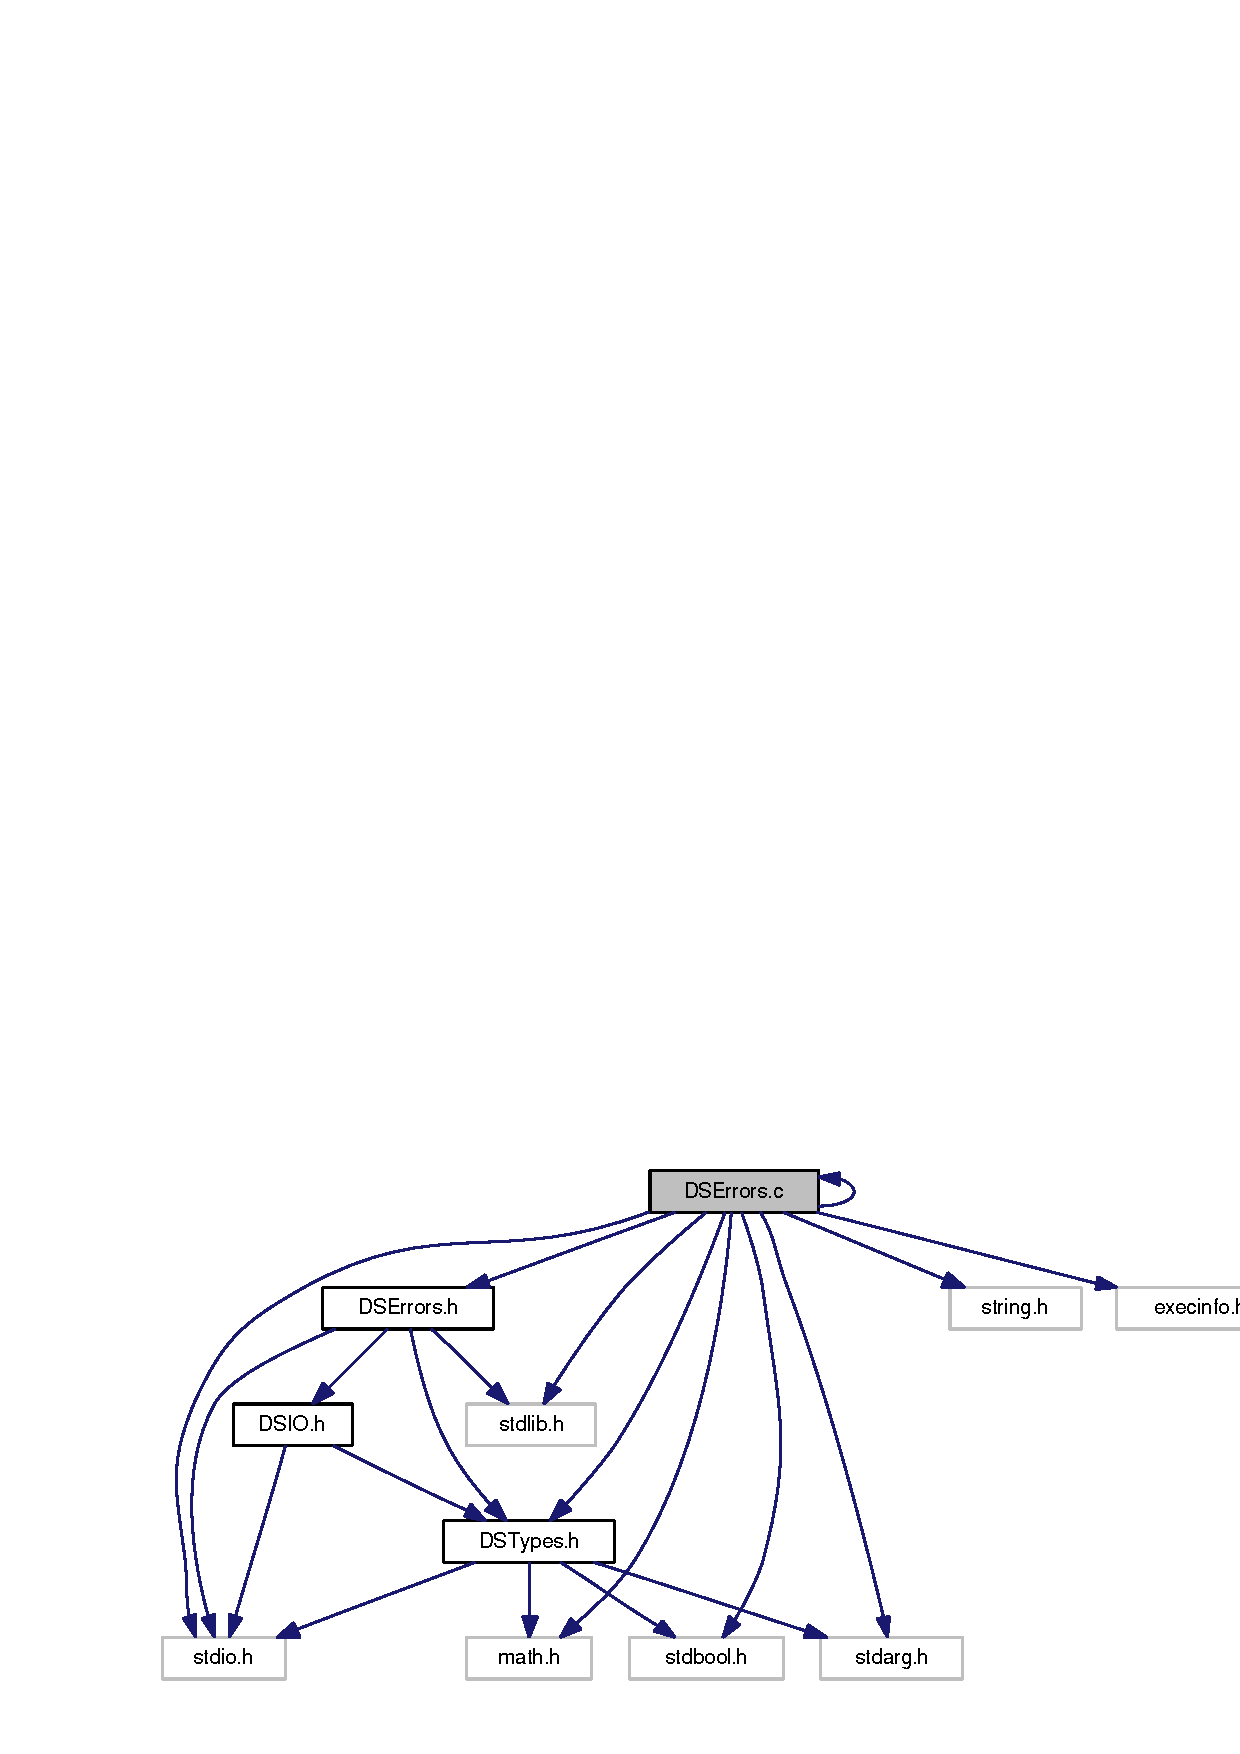
\includegraphics[width=308pt]{_d_s_errors_8c__incl}
\end{center}
\end{figure}
This graph shows which files directly or indirectly include this file:\nopagebreak
\begin{figure}[H]
\begin{center}
\leavevmode
\includegraphics[width=67pt]{_d_s_errors_8c__dep__incl}
\end{center}
\end{figure}
\subsection*{Defines}
\begin{DoxyCompactItemize}
\item 
\hypertarget{_d_s_errors_8c_af86fc5cdaf2e11d46f2aa2201d74f0a4}{
\#define {\bfseries STACK\_\-TRACE\_\-NUM}~10}
\label{_d_s_errors_8c_af86fc5cdaf2e11d46f2aa2201d74f0a4}

\item 
\hypertarget{_d_s_errors_8c_a849adc9d20371988bb26f86618fa75ba}{
\#define {\bfseries MSIZE}~1500}
\label{_d_s_errors_8c_a849adc9d20371988bb26f86618fa75ba}

\end{DoxyCompactItemize}
\subsection*{Functions}
\begin{DoxyCompactItemize}
\item 
\hypertarget{_d_s_errors_8c_a835a62d5dadb2499cc180b27fb77868e}{
void {\bfseries DSErrorSetPrintFunction} (void($\ast$function)(const char $\ast$restrict))}
\label{_d_s_errors_8c_a835a62d5dadb2499cc180b27fb77868e}

\item 
\hypertarget{_d_s_errors_8c_a4b43fbbf45cfa65d56dbe161948afe18}{
void {\bfseries DSErrorSetErrorFile} (FILE $\ast$aFile)}
\label{_d_s_errors_8c_a4b43fbbf45cfa65d56dbe161948afe18}

\item 
void \hyperlink{_d_s_errors_8c_a363f9c264b785ec509da1b11af9ae314}{DSErrorFunction} (const char $\ast$M\_\-DS\_\-Message, char A\_\-DS\_\-ACTION, const char $\ast$FILEN, int LINE, const char $\ast$FUNC)
\begin{DoxyCompactList}\small\item\em Implicit error handling function. Called by DSError which automatically adds file and line arguments. \item\end{DoxyCompactList}\end{DoxyCompactItemize}


\subsection{Detailed Description}
Implementation file with functions for error and exception handling. This file specifies the design space standard for error handling. Contained here are the necessary macros and functions to report the errors throughout the design space library. The DSErrorFunction allows different behaviors; the default behavior, errors are printed to the DSIOErrorFile, which is set to stderr by default. This behavior can be changed by setting changing DSPostWarning, DSPostError and DSPostFatalError function pointers.

\begin{DoxySeeAlso}{See also}
\hyperlink{_d_s_i_o_8h_af8405bae84409f99d5fa564ebaff4c91}{DSIOErrorFile} 

\hyperlink{_d_s_i_o_8h_af12cf032b729ba022698fadaccfea33d}{DSPostWarning} 

\hyperlink{_d_s_i_o_8h_a40c3f80fe9e5002beb7d258e4f89c8d2}{DSPostError} 

\hyperlink{_d_s_i_o_8h_a41b7b42028f3c25f17ca479154c7492d}{DSPostFatalError}
\end{DoxySeeAlso}
Copyright (C) 2011 Jason Lomnitz.\par
\par


This file is part of the Design Space Toolbox V2 (C Library).

The Design Space Toolbox V2 is free software: you can redistribute it and/or modify it under the terms of the GNU General Public License as published by the Free Software Foundation, either version 3 of the License, or (at your option) any later version.

The Design Space Toolbox V2 is distributed in the hope that it will be useful, but WITHOUT ANY WARRANTY; without even the implied warranty of MERCHANTABILITY or FITNESS FOR A PARTICULAR PURPOSE. See the GNU General Public License for more details.

You should have received a copy of the GNU General Public License along with the Design Space Toolbox. If not, see $<$\href{http://www.gnu.org/licenses/}{\tt http://www.gnu.org/licenses/}$>$.

\begin{DoxyAuthor}{Author}
Jason Lomnitz. 
\end{DoxyAuthor}
\begin{DoxyDate}{Date}
2011 
\end{DoxyDate}


\subsection{Function Documentation}
\hypertarget{_d_s_errors_8c_a363f9c264b785ec509da1b11af9ae314}{
\index{DSErrors.c@{DSErrors.c}!DSErrorFunction@{DSErrorFunction}}
\index{DSErrorFunction@{DSErrorFunction}!DSErrors.c@{DSErrors.c}}
\subsubsection[{DSErrorFunction}]{\setlength{\rightskip}{0pt plus 5cm}void DSErrorFunction (const char $\ast$ {\em M\_\-DS\_\-Message}, \/  char {\em A\_\-DS\_\-ACTION}, \/  const char $\ast$ {\em FILEN}, \/  int {\em LINE}, \/  const char $\ast$ {\em FUNC})}}
\label{_d_s_errors_8c_a363f9c264b785ec509da1b11af9ae314}


Implicit error handling function. Called by DSError which automatically adds file and line arguments. 

This function is called implicity when using the DSError macro. The DSError adds the FILE and LINE argument, to report the error/warning at the appropriate file and line.

\begin{DoxySeeAlso}{See also}
\hyperlink{_d_s_errors_8h_a09b28eb2b01986855910ca97dfe91144}{DSError} 

\hyperlink{group___a___d_s___actions}{Actions for DS Errors.} 
\end{DoxySeeAlso}

\hypertarget{_d_s_errors_8h}{
\section{DSErrors.h File Reference}
\label{_d_s_errors_8h}\index{DSErrors.h@{DSErrors.h}}
}


Header file with functions for error and exception handling.  


{\ttfamily \#include $<$stdio.h$>$}\par
{\ttfamily \#include $<$stdlib.h$>$}\par
{\ttfamily \#include \char`\"{}DSTypes.h\char`\"{}}\par
{\ttfamily \#include \char`\"{}DSIO.h\char`\"{}}\par
Include dependency graph for DSErrors.h:\nopagebreak
\begin{figure}[H]
\begin{center}
\leavevmode
\includegraphics[width=179pt]{_d_s_errors_8h__incl}
\end{center}
\end{figure}
This graph shows which files directly or indirectly include this file:\subsection*{Defines}
\begin{DoxyCompactItemize}
\item 
\hypertarget{group___m___d_s___messages_gadd043ccc956aaee49b9c646f940c167b}{
\#define \hyperlink{group___m___d_s___messages_gadd043ccc956aaee49b9c646f940c167b}{M\_\-DS\_\-NOFILE}~\char`\"{}File not found\char`\"{}}
\label{group___m___d_s___messages_gadd043ccc956aaee49b9c646f940c167b}

\begin{DoxyCompactList}\small\item\em Message for no file found. \item\end{DoxyCompactList}\item 
\hypertarget{group___m___d_s___messages_ga0d502db70be066b76fa94dc1eb9ef75c}{
\#define \hyperlink{group___m___d_s___messages_ga0d502db70be066b76fa94dc1eb9ef75c}{M\_\-DS\_\-NULL}~\char`\"{}NULL pointer\char`\"{}}
\label{group___m___d_s___messages_ga0d502db70be066b76fa94dc1eb9ef75c}

\begin{DoxyCompactList}\small\item\em Message for NULL pointer. \item\end{DoxyCompactList}\item 
\hypertarget{group___m___d_s___messages_ga05191be522c29caa6f80baddfb2a109c}{
\#define \hyperlink{group___m___d_s___messages_ga05191be522c29caa6f80baddfb2a109c}{M\_\-DS\_\-NOFORMAT}~\char`\"{}Format not known\char`\"{}}
\label{group___m___d_s___messages_ga05191be522c29caa6f80baddfb2a109c}

\begin{DoxyCompactList}\small\item\em Message for unknown format. \item\end{DoxyCompactList}\item 
\hypertarget{_d_s_errors_8h_a09ad9583c7a29550cc6a9a7606bf71fb}{
\#define \hyperlink{_d_s_errors_8h_a09ad9583c7a29550cc6a9a7606bf71fb}{M\_\-DS\_\-WRONG}~\char`\"{}Inconsistent data\char`\"{}}
\label{_d_s_errors_8h_a09ad9583c7a29550cc6a9a7606bf71fb}

\begin{DoxyCompactList}\small\item\em Message for inconsistent data being used. \item\end{DoxyCompactList}\item 
\hypertarget{group___m___d_s___messages_ga33ff33533363ff94af03b832587f47c6}{
\#define \hyperlink{group___m___d_s___messages_ga33ff33533363ff94af03b832587f47c6}{M\_\-DS\_\-EXISTS}~\char`\"{}Data already exists\char`\"{}}
\label{group___m___d_s___messages_ga33ff33533363ff94af03b832587f47c6}

\begin{DoxyCompactList}\small\item\em Message for data aleady existing. \item\end{DoxyCompactList}\item 
\hypertarget{_d_s_errors_8h_afd9c8dc0e9bf6bdaa09c3edd3125fc89}{
\#define \hyperlink{_d_s_errors_8h_afd9c8dc0e9bf6bdaa09c3edd3125fc89}{M\_\-DS\_\-NOTHREAD}~\char`\"{}Thread not created\char`\"{}}
\label{_d_s_errors_8h_afd9c8dc0e9bf6bdaa09c3edd3125fc89}

\begin{DoxyCompactList}\small\item\em Message for no thread created. \item\end{DoxyCompactList}\item 
\hypertarget{group___m___d_s___messages_ga47106b8852d8baaf66a0e7f9bd67d36b}{
\#define \hyperlink{group___m___d_s___messages_ga47106b8852d8baaf66a0e7f9bd67d36b}{M\_\-DS\_\-MALLOC}~\char`\"{}Memory alloc failed\char`\"{}}
\label{group___m___d_s___messages_ga47106b8852d8baaf66a0e7f9bd67d36b}

\begin{DoxyCompactList}\small\item\em Message for failure to allocate data. \item\end{DoxyCompactList}\item 
\hypertarget{group___m___d_s___messages_ga79c48eacc7951aa68e4d094f0989faac}{
\#define \hyperlink{group___m___d_s___messages_ga79c48eacc7951aa68e4d094f0989faac}{M\_\-DS\_\-NOT\_\-IMPL}~\char`\"{}Functionality not implemented\char`\"{}}
\label{group___m___d_s___messages_ga79c48eacc7951aa68e4d094f0989faac}

\begin{DoxyCompactList}\small\item\em Message for a feature not yet implemented. \item\end{DoxyCompactList}\item 
\hypertarget{_d_s_errors_8h_a2073c22dca19fb517f4b709ea58c7c2a}{
\#define \hyperlink{_d_s_errors_8h_a2073c22dca19fb517f4b709ea58c7c2a}{M\_\-DS\_\-PARSE}~\char`\"{}Could not parse data\char`\"{}}
\label{_d_s_errors_8h_a2073c22dca19fb517f4b709ea58c7c2a}

\begin{DoxyCompactList}\small\item\em Message for an error during parsing. \item\end{DoxyCompactList}\item 
\hypertarget{group___a___d_s___actions_ga83fd1c7379ac085b8a9550b8d64f3449}{
\#define \hyperlink{group___a___d_s___actions_ga83fd1c7379ac085b8a9550b8d64f3449}{A\_\-DS\_\-NOERROR}~0}
\label{group___a___d_s___actions_ga83fd1c7379ac085b8a9550b8d64f3449}

\begin{DoxyCompactList}\small\item\em Value for no error. \item\end{DoxyCompactList}\item 
\hypertarget{group___a___d_s___actions_gad61c12e433c47da75f4322d9358c3617}{
\#define \hyperlink{group___a___d_s___actions_gad61c12e433c47da75f4322d9358c3617}{A\_\-DS\_\-WARN}~-\/1}
\label{group___a___d_s___actions_gad61c12e433c47da75f4322d9358c3617}

\begin{DoxyCompactList}\small\item\em Value for a warning. \item\end{DoxyCompactList}\item 
\hypertarget{group___a___d_s___actions_gabaa9a22cc1abc78916b99695489f8df8}{
\#define \hyperlink{group___a___d_s___actions_gabaa9a22cc1abc78916b99695489f8df8}{A\_\-DS\_\-ERROR}~-\/2}
\label{group___a___d_s___actions_gabaa9a22cc1abc78916b99695489f8df8}

\begin{DoxyCompactList}\small\item\em Value for an error. \item\end{DoxyCompactList}\item 
\hypertarget{group___a___d_s___actions_gad3e083f0c8d34073d3597724c2a264f6}{
\#define \hyperlink{group___a___d_s___actions_gad3e083f0c8d34073d3597724c2a264f6}{A\_\-DS\_\-FATAL}~-\/3}
\label{group___a___d_s___actions_gad3e083f0c8d34073d3597724c2a264f6}

\begin{DoxyCompactList}\small\item\em Value for a fatal error, kills program. \item\end{DoxyCompactList}\item 
\hypertarget{group___a___d_s___actions_gafc6d540dbb27b62f52427a845a33212f}{
\#define \hyperlink{group___a___d_s___actions_gafc6d540dbb27b62f52427a845a33212f}{A\_\-DS\_\-KILLNOW}~A\_\-DS\_\-FATAL}
\label{group___a___d_s___actions_gafc6d540dbb27b62f52427a845a33212f}

\begin{DoxyCompactList}\small\item\em DEPRECATED: \item\end{DoxyCompactList}\item 
\#define \hyperlink{_d_s_errors_8h_a09b28eb2b01986855910ca97dfe91144}{DSError}(M\_\-DS\_\-Message, A\_\-DS\_\-Action)~DSErrorFunction(M\_\-DS\_\-Message, A\_\-DS\_\-Action, \_\-\_\-FILE\_\-\_\-, \_\-\_\-LINE\_\-\_\-, \_\-\_\-func\_\-\_\-)
\begin{DoxyCompactList}\small\item\em Error reporting macro. \item\end{DoxyCompactList}\end{DoxyCompactItemize}
\subsection*{Functions}
\begin{DoxyCompactItemize}
\item 
void \hyperlink{_d_s_errors_8h_a363f9c264b785ec509da1b11af9ae314}{DSErrorFunction} (const char $\ast$M\_\-DS\_\-Message, char A\_\-DS\_\-ACTION, const char $\ast$FILEN, int LINE, const char $\ast$FUNC)
\begin{DoxyCompactList}\small\item\em Implicit error handling function. Called by DSError which automatically adds file and line arguments. \item\end{DoxyCompactList}\end{DoxyCompactItemize}


\subsection{Detailed Description}
Header file with functions for error and exception handling. This file specifies the design space standard for error handling. Contained here are the necessary macros and functions to succesfully report the errors throughout the design space library.

Copyright (C) 2011 Jason Lomnitz.\par
\par


This file is part of the Design Space Toolbox V2 (C Library).

The Design Space Toolbox V2 is free software: you can redistribute it and/or modify it under the terms of the GNU General Public License as published by the Free Software Foundation, either version 3 of the License, or (at your option) any later version.

The Design Space Toolbox V2 is distributed in the hope that it will be useful, but WITHOUT ANY WARRANTY; without even the implied warranty of MERCHANTABILITY or FITNESS FOR A PARTICULAR PURPOSE. See the GNU General Public License for more details.

You should have received a copy of the GNU General Public License along with the Design Space Toolbox. If not, see $<$\href{http://www.gnu.org/licenses/}{\tt http://www.gnu.org/licenses/}$>$.

\begin{DoxyAuthor}{Author}
Jason Lomnitz. 
\end{DoxyAuthor}
\begin{DoxyDate}{Date}
2011 
\end{DoxyDate}


\subsection{Define Documentation}
\hypertarget{_d_s_errors_8h_a09b28eb2b01986855910ca97dfe91144}{
\index{DSErrors.h@{DSErrors.h}!DSError@{DSError}}
\index{DSError@{DSError}!DSErrors.h@{DSErrors.h}}
\subsubsection[{DSError}]{\setlength{\rightskip}{0pt plus 5cm}\#define DSError(M\_\-DS\_\-Message, \/  A\_\-DS\_\-Action)~DSErrorFunction(M\_\-DS\_\-Message, A\_\-DS\_\-Action, \_\-\_\-FILE\_\-\_\-, \_\-\_\-LINE\_\-\_\-, \_\-\_\-func\_\-\_\-)}}
\label{_d_s_errors_8h_a09b28eb2b01986855910ca97dfe91144}


Error reporting macro. 

Definition of the error reporting macro used within the DesignSpace C toolbox, this is a define which takes a string, which may be a standard message, and an action and reports it via the standard warning and error posting functions in the standard IO functions. A default behavior of the DSError macro posts warning and errors to stderr, while a fatal error posts the error to stderr and aborts the program.

\begin{DoxySeeAlso}{See also}
\hyperlink{_d_s_i_o_8h_af12cf032b729ba022698fadaccfea33d}{DSPostWarning} 

\hyperlink{_d_s_i_o_8h_a40c3f80fe9e5002beb7d258e4f89c8d2}{DSPostError} 

\hyperlink{_d_s_i_o_8h_a41b7b42028f3c25f17ca479154c7492d}{DSPostFatalError}

\hyperlink{group___m___d_s___messages}{Messages for DS Errors.} 

\hyperlink{group___a___d_s___actions}{Actions for DS Errors.} 
\end{DoxySeeAlso}


\subsection{Function Documentation}
\hypertarget{_d_s_errors_8h_a363f9c264b785ec509da1b11af9ae314}{
\index{DSErrors.h@{DSErrors.h}!DSErrorFunction@{DSErrorFunction}}
\index{DSErrorFunction@{DSErrorFunction}!DSErrors.h@{DSErrors.h}}
\subsubsection[{DSErrorFunction}]{\setlength{\rightskip}{0pt plus 5cm}void DSErrorFunction (const char $\ast$ {\em M\_\-DS\_\-Message}, \/  char {\em A\_\-DS\_\-ACTION}, \/  const char $\ast$ {\em FILEN}, \/  int {\em LINE}, \/  const char $\ast$ {\em FUNC})}}
\label{_d_s_errors_8h_a363f9c264b785ec509da1b11af9ae314}


Implicit error handling function. Called by DSError which automatically adds file and line arguments. 

This function is called implicity when using the DSError macro. The DSError adds the FILE, LINE and FUNC arguments, to report the error/warning at the appropriate file, line and function.


\begin{DoxyParams}{Parameters}
\item[{\em M\_\-DS\_\-Message}]A string containing the error message. \item[{\em A\_\-DS\_\-ACTION}]A character representing an error code as described in A\_\-DS\_\-Actions. \item[{\em FILEN}]A string with the name of the file where the error was reported. \item[{\em LINE}]An integer with the line number in the file where the error was reported. \item[{\em FUNC}]A string with the name of the function where the error was reported.\end{DoxyParams}
\begin{DoxySeeAlso}{See also}
\hyperlink{_d_s_errors_8h_a09b28eb2b01986855910ca97dfe91144}{DSError} 

\hyperlink{group___a___d_s___actions}{Actions for DS Errors.} 
\end{DoxySeeAlso}

\hypertarget{_d_s_i_o_8c}{
\section{DSIO.c File Reference}
\label{_d_s_i_o_8c}\index{DSIO.c@{DSIO.c}}
}


Implementation file with standard input and output functions.  


{\ttfamily \#include $<$stdio.h$>$}\par
{\ttfamily \#include $<$string.h$>$}\par
{\ttfamily \#include \char`\"{}DSIO.h\char`\"{}}\par
{\ttfamily \#include \char`\"{}DSMemoryManager.h\char`\"{}}\par
{\ttfamily \#include \char`\"{}DSVariable.h\char`\"{}}\par
{\ttfamily \#include \char`\"{}DSMatrix.h\char`\"{}}\par
{\ttfamily \#include \char`\"{}DSMatrixArray.h\char`\"{}}\par
{\ttfamily \#include \char`\"{}DSGMASystem.h\char`\"{}}\par
{\ttfamily \#include \char`\"{}DSSSystem.h\char`\"{}}\par
{\ttfamily \#include \char`\"{}DSCase.h\char`\"{}}\par
Include dependency graph for DSIO.c:\nopagebreak
\begin{figure}[H]
\begin{center}
\leavevmode
\includegraphics[width=175pt]{_d_s_i_o_8c__incl}
\end{center}
\end{figure}
\subsection*{Defines}
\begin{DoxyCompactItemize}
\item 
\hypertarget{group___d_s___i_o___t_a_g___t_y_p_e_s_gad9110308f40b701fa7a8ac65d48716c6}{
\#define {\bfseries DS\_\-IO\_\-TAG\_\-TYPE\_\-Matrix}~\char`\"{}$\backslash$\char`\"{}\hyperlink{struct_d_s_matrix}{DSMatrix}$\backslash$\char`\"{}\char`\"{}}
\label{group___d_s___i_o___t_a_g___t_y_p_e_s_gad9110308f40b701fa7a8ac65d48716c6}

\item 
\hypertarget{group___d_s___i_o___t_a_g___t_y_p_e_s_ga26f0a22ebdc3e22f453d06fe231c3477}{
\#define {\bfseries DS\_\-IO\_\-TAG\_\-TYPE\_\-MatrixArray}~\char`\"{}$\backslash$\char`\"{}\hyperlink{struct_d_s_matrix_array}{DSMatrixArray}$\backslash$\char`\"{}\char`\"{}}
\label{group___d_s___i_o___t_a_g___t_y_p_e_s_ga26f0a22ebdc3e22f453d06fe231c3477}

\item 
\hypertarget{group___d_s___i_o___t_a_g___t_y_p_e_s_ga33b8d327f394e774d81e2702d27673ec}{
\#define {\bfseries DS\_\-IO\_\-TAG\_\-TYPE\_\-VariablePool}~\char`\"{}$\backslash$\char`\"{}\hyperlink{struct_d_s_variable_pool}{DSVariablePool}$\backslash$\char`\"{}\char`\"{}}
\label{group___d_s___i_o___t_a_g___t_y_p_e_s_ga33b8d327f394e774d81e2702d27673ec}

\item 
\hypertarget{group___d_s___i_o___t_a_g___t_y_p_e_s_ga48168f56a3bd807c4f677f50236f3fd9}{
\#define {\bfseries DS\_\-IO\_\-TAG\_\-TYPE\_\-Dictionary}~\char`\"{}$\backslash$\char`\"{}\hyperlink{struct_d_s_dictionary}{DSDictionary}$\backslash$\char`\"{}\char`\"{}}
\label{group___d_s___i_o___t_a_g___t_y_p_e_s_ga48168f56a3bd807c4f677f50236f3fd9}

\item 
\hypertarget{group___d_s___i_o___t_a_g___t_y_p_e_s_ga9e91e3c5dab3046aa518bf339e1f13e0}{
\#define {\bfseries DS\_\-IO\_\-TAG\_\-TYPE\_\-SSystem}~\char`\"{}$\backslash$\char`\"{}\hyperlink{struct_d_s_s_system}{DSSSystem}$\backslash$\char`\"{}\char`\"{}}
\label{group___d_s___i_o___t_a_g___t_y_p_e_s_ga9e91e3c5dab3046aa518bf339e1f13e0}

\item 
\hypertarget{group___d_s___i_o___t_a_g___t_y_p_e_s_gab40a361af4d08bed8503c9a681f5a51a}{
\#define {\bfseries DS\_\-IO\_\-TAG\_\-TYPE\_\-Case}~\char`\"{}$\backslash$\char`\"{}\hyperlink{struct_d_s_case}{DSCase}$\backslash$\char`\"{}\char`\"{}}
\label{group___d_s___i_o___t_a_g___t_y_p_e_s_gab40a361af4d08bed8503c9a681f5a51a}

\item 
\hypertarget{group___d_s___i_o___t_a_g___t_y_p_e_s_ga4f6f8a8ee7b2387292daf78f6b5fe7ef}{
\#define {\bfseries DS\_\-IO\_\-TAG\_\-TYPE\_\-DesignSpace}~\char`\"{}$\backslash$\char`\"{}\hyperlink{struct_d_s_design_space}{DSDesignSpace}$\backslash$\char`\"{}\char`\"{}}
\label{group___d_s___i_o___t_a_g___t_y_p_e_s_ga4f6f8a8ee7b2387292daf78f6b5fe7ef}

\end{DoxyCompactItemize}
\subsection*{Functions}
\begin{DoxyCompactItemize}
\item 
void \hyperlink{_d_s_i_o_8c_a71e4035e82cf614f1be280b127213ca6}{DSIOSetErrorFile} (FILE $\ast$aFile)
\begin{DoxyCompactList}\small\item\em Function to assign default error file. \item\end{DoxyCompactList}\item 
void \hyperlink{_d_s_i_o_8c_aaa699261767672e938101744e4032249}{DSIOSetPrintFunction} (int($\ast$printFunction)(const char $\ast$,...))
\begin{DoxyCompactList}\small\item\em Function to assign default printf function. \item\end{DoxyCompactList}\item 
void \hyperlink{_d_s_i_o_8c_a37a5183ebd833f0cf9bc2ed19e43fb84}{DSIOSetPostWarningFunction} (void($\ast$warningFunction)(const char $\ast$message))
\begin{DoxyCompactList}\small\item\em Function to assign default warning posting function. \item\end{DoxyCompactList}\item 
void \hyperlink{_d_s_i_o_8c_a8c9be4c3d8b1802aa5295165c3f0b861}{DSIOSetPostErrorFunction} (void($\ast$errorFunction)(const char $\ast$message))
\begin{DoxyCompactList}\small\item\em Function to assign default error posting function. \item\end{DoxyCompactList}\item 
void \hyperlink{_d_s_i_o_8c_a1fbcb57d54a5ac852484b43e317aa43f}{DSIOSetPostFatalErrorFunction} (void($\ast$fatalErrorFunction)(const char $\ast$message))
\begin{DoxyCompactList}\small\item\em Function to assign default fatal error posting function. \item\end{DoxyCompactList}\item 
void \hyperlink{_d_s_i_o_8c_a6cb102dc8b55faa48dca0c51fa0fb517}{DSIOSetCaseJSONOptions} (const DSUInteger options)
\begin{DoxyCompactList}\small\item\em Function that sets the conversion options for a \hyperlink{struct_d_s_case}{DSCase} to JSON format. \item\end{DoxyCompactList}\item 
void \hyperlink{_d_s_i_o_8c_a2a957ad88bd1a2f4d5b0ed616344c7ac}{DSIOSetSSystemJSONOptions} (const DSUInteger options)
\begin{DoxyCompactList}\small\item\em Function that sets the conversion options for a \hyperlink{struct_d_s_s_system}{DSSSystem} to JSON format. \item\end{DoxyCompactList}\item 
char $\ast$ \hyperlink{_d_s_i_o_8c_a754fa75644786b862aabc2660f191d14}{DSVariablePoolStringInJSONFormat} (const \hyperlink{struct_d_s_variable_pool}{DSVariablePool} $\ast$pool)
\begin{DoxyCompactList}\small\item\em Function to convert a \hyperlink{struct_d_s_variable_pool}{DSVariablePool} into a JSON formatted string. \item\end{DoxyCompactList}\item 
char $\ast$ \hyperlink{_d_s_i_o_8c_a6a9e23721286736288947c43461f12ae}{DSMatrixStringInJSONFormat} (const \hyperlink{struct_d_s_matrix}{DSMatrix} $\ast$matrix)
\begin{DoxyCompactList}\small\item\em Function to convert a \hyperlink{struct_d_s_matrix}{DSMatrix} into a JSON formatted string. \item\end{DoxyCompactList}\item 
char $\ast$ \hyperlink{_d_s_i_o_8c_ab8cae51e1c113fc52e1da34fffdc6f40}{DSMatrixArrayStringInJSONFormat} (const \hyperlink{struct_d_s_matrix_array}{DSMatrixArray} $\ast$array)
\begin{DoxyCompactList}\small\item\em Function to convert a \hyperlink{struct_d_s_matrix_array}{DSMatrixArray} into a JSON formatted string. \item\end{DoxyCompactList}\item 
char $\ast$ \hyperlink{_d_s_i_o_8c_a2679d81ab81c12c930cbb7a5e2791d73}{DSSSystemStringInJSONFormat} (const \hyperlink{struct_d_s_s_system}{DSSSystem} $\ast$ssys)
\begin{DoxyCompactList}\small\item\em Function to convert a \hyperlink{struct_d_s_s_system}{DSSSystem} into a JSON formatted string. \item\end{DoxyCompactList}\item 
char $\ast$ \hyperlink{_d_s_i_o_8c_a08dbac8a5ae623c94cf44bd620e46060}{DSCaseStringInJSONFormat} (const \hyperlink{struct_d_s_case}{DSCase} $\ast$aCase)
\begin{DoxyCompactList}\small\item\em Function to convert a \hyperlink{struct_d_s_case}{DSCase} into a JSON formatted string. \item\end{DoxyCompactList}\end{DoxyCompactItemize}
\subsection*{Variables}
\begin{DoxyCompactItemize}
\item 
int($\ast$ \hyperlink{_d_s_i_o_8c_a01ab8215975bf8e2086ad342cfa6be26}{DSPrintf} )(const char $\ast$,...)
\begin{DoxyCompactList}\small\item\em Pointer to a function determining how messages are printed. \item\end{DoxyCompactList}\item 
void($\ast$ \hyperlink{_d_s_i_o_8c_af12cf032b729ba022698fadaccfea33d}{DSPostWarning} )(const char $\ast$message)
\begin{DoxyCompactList}\small\item\em Pointer to a function determining how warning are handled. \item\end{DoxyCompactList}\item 
void($\ast$ \hyperlink{_d_s_i_o_8c_a40c3f80fe9e5002beb7d258e4f89c8d2}{DSPostError} )(const char $\ast$message)
\begin{DoxyCompactList}\small\item\em Pointer to a function determining how errors are handled. \item\end{DoxyCompactList}\item 
void($\ast$ \hyperlink{_d_s_i_o_8c_a41b7b42028f3c25f17ca479154c7492d}{DSPostFatalError} )(const char $\ast$message)
\begin{DoxyCompactList}\small\item\em Pointer to a function determining how fatal errors are handled. \item\end{DoxyCompactList}\item 
FILE $\ast$ \hyperlink{_d_s_i_o_8c_af8405bae84409f99d5fa564ebaff4c91}{DSIOErrorFile}
\begin{DoxyCompactList}\small\item\em FILE pointer used for default error/warning printing. \item\end{DoxyCompactList}\item 
DSUInteger \hyperlink{_d_s_i_o_8c_a54a8bab51a88d9b670634fbe6174c865}{DSSSystemPrintingOptions}
\begin{DoxyCompactList}\small\item\em Variable with flags controlling S-\/System to JSON string conversion. \item\end{DoxyCompactList}\item 
DSUInteger \hyperlink{_d_s_i_o_8c_a3d4acaf78ffb997163a7705876c1feb1}{DSCasePrintingOptions}
\begin{DoxyCompactList}\small\item\em Variable with flags controlling the conversion of a Case to a JSON string. \item\end{DoxyCompactList}\end{DoxyCompactItemize}


\subsection{Detailed Description}
Implementation file with standard input and output functions. Copyright (C) 2011 Jason Lomnitz.

This file is part of the Design Space Toolbox V2 (C Library).

The Design Space Toolbox V2 is free software: you can redistribute it and/or modify it under the terms of the GNU General Public License as published by the Free Software Foundation, either version 3 of the License, or (at your option) any later version.

The Design Space Toolbox V2 is distributed in the hope that it will be useful, but WITHOUT ANY WARRANTY; without even the implied warranty of MERCHANTABILITY or FITNESS FOR A PARTICULAR PURPOSE. See the GNU General Public License for more details.

You should have received a copy of the GNU General Public License along with the Design Space Toolbox. If not, see $<$\href{http://www.gnu.org/licenses/}{\tt http://www.gnu.org/licenses/}$>$.

\begin{DoxyAuthor}{Author}
Jason Lomnitz. 
\end{DoxyAuthor}
\begin{DoxyDate}{Date}
2011 
\end{DoxyDate}


\subsection{Function Documentation}
\hypertarget{_d_s_i_o_8c_a08dbac8a5ae623c94cf44bd620e46060}{
\index{DSIO.c@{DSIO.c}!DSCaseStringInJSONFormat@{DSCaseStringInJSONFormat}}
\index{DSCaseStringInJSONFormat@{DSCaseStringInJSONFormat}!DSIO.c@{DSIO.c}}
\subsubsection[{DSCaseStringInJSONFormat}]{\setlength{\rightskip}{0pt plus 5cm}char$\ast$ DSCaseStringInJSONFormat (const {\bf DSCase} $\ast$ {\em aCase})}}
\label{_d_s_i_o_8c_a08dbac8a5ae623c94cf44bd620e46060}


Function to convert a \hyperlink{struct_d_s_case}{DSCase} into a JSON formatted string. 

This function is used to convert a \hyperlink{struct_d_s_case}{DSCase} into a JSON object. The \hyperlink{struct_d_s_case}{DSCase} is represented with a set of objects, where each object is a field of the \hyperlink{struct_d_s_case}{DSCase} object. The default behavior exports all of the fields, this behavior can be overwritten by changing the \hyperlink{struct_d_s_case}{DSCase} conversion options.


\begin{DoxyParams}{Parameters}
\item[{\em aCase}]A \hyperlink{struct_d_s_case}{DSCase} that will be used to create the JSON object.\end{DoxyParams}
\begin{DoxyReturn}{Returns}
A C string with the JSON formatted data. If NULL, the conversion failed.
\end{DoxyReturn}
\begin{DoxySeeAlso}{See also}
\hyperlink{_d_s_i_o_8c_a6cb102dc8b55faa48dca0c51fa0fb517}{DSIOSetCaseJSONOptions()} 
\end{DoxySeeAlso}
\hypertarget{_d_s_i_o_8c_a6cb102dc8b55faa48dca0c51fa0fb517}{
\index{DSIO.c@{DSIO.c}!DSIOSetCaseJSONOptions@{DSIOSetCaseJSONOptions}}
\index{DSIOSetCaseJSONOptions@{DSIOSetCaseJSONOptions}!DSIO.c@{DSIO.c}}
\subsubsection[{DSIOSetCaseJSONOptions}]{\setlength{\rightskip}{0pt plus 5cm}void DSIOSetCaseJSONOptions (const DSUInteger {\em options})}}
\label{_d_s_i_o_8c_a6cb102dc8b55faa48dca0c51fa0fb517}


Function that sets the conversion options for a \hyperlink{struct_d_s_case}{DSCase} to JSON format. 

This function is used to overwrite the default export behavior of the \hyperlink{struct_d_s_case}{DSCase} object. The default behavior converts all of the data fields of the \hyperlink{struct_d_s_case}{DSCase} into a JSON format, these options can be changed so the JSON conversion only includes some fields, such as excluding the conditions, excluding the S-\/System, etc.


\begin{DoxyParams}{Parameters}
\item[{\em options}]A DSUInteger with the option flags, as specified by the \hyperlink{struct_d_s_case}{DSCase} options.\end{DoxyParams}
\begin{DoxySeeAlso}{See also}
\hyperlink{group___d_s___c_a_s_e___j_s_o_n___o_p_t_i_o_n_s}{Options for JSON conversion of DSCase object.} 
\end{DoxySeeAlso}
\hypertarget{_d_s_i_o_8c_a71e4035e82cf614f1be280b127213ca6}{
\index{DSIO.c@{DSIO.c}!DSIOSetErrorFile@{DSIOSetErrorFile}}
\index{DSIOSetErrorFile@{DSIOSetErrorFile}!DSIO.c@{DSIO.c}}
\subsubsection[{DSIOSetErrorFile}]{\setlength{\rightskip}{0pt plus 5cm}void DSIOSetErrorFile (FILE $\ast$ {\em aFile})}}
\label{_d_s_i_o_8c_a71e4035e82cf614f1be280b127213ca6}


Function to assign default error file. 

This function is used to assign the default error file, DSIOErrorFile. Changing the error file should be done via this function, as it circumvents potential problems associated with dynamic linking.


\begin{DoxyParams}{Parameters}
\item[{\em aFile}]A FILE $\ast$ that will be used to write error messages when the default error posting mechanism is used.\end{DoxyParams}
\begin{DoxySeeAlso}{See also}
\hyperlink{_d_s_i_o_8h_a37a5183ebd833f0cf9bc2ed19e43fb84}{DSIOSetPostWarningFunction} 

\hyperlink{_d_s_i_o_8h_a8c9be4c3d8b1802aa5295165c3f0b861}{DSIOSetPostErrorFunction} 

\hyperlink{_d_s_i_o_8h_a1fbcb57d54a5ac852484b43e317aa43f}{DSIOSetPostFatalErrorFunction} 

\hyperlink{_d_s_errors_8h_a09b28eb2b01986855910ca97dfe91144}{DSError} 
\end{DoxySeeAlso}
\hypertarget{_d_s_i_o_8c_a8c9be4c3d8b1802aa5295165c3f0b861}{
\index{DSIO.c@{DSIO.c}!DSIOSetPostErrorFunction@{DSIOSetPostErrorFunction}}
\index{DSIOSetPostErrorFunction@{DSIOSetPostErrorFunction}!DSIO.c@{DSIO.c}}
\subsubsection[{DSIOSetPostErrorFunction}]{\setlength{\rightskip}{0pt plus 5cm}void DSIOSetPostErrorFunction (void($\ast$)(const char $\ast$message) {\em errorFunction})}}
\label{_d_s_i_o_8c_a8c9be4c3d8b1802aa5295165c3f0b861}


Function to assign default error posting function. 

This function is used to assign the function that handles the errors generated from the design space toolbox. Internally, it assigns the global variable DSPostError which points to a function.


\begin{DoxyParams}{Parameters}
\item[{\em errorFunction}]A pointer to a function of the form void function(const char $\ast$). If NULL, default behavior is restored. \end{DoxyParams}
\hypertarget{_d_s_i_o_8c_a1fbcb57d54a5ac852484b43e317aa43f}{
\index{DSIO.c@{DSIO.c}!DSIOSetPostFatalErrorFunction@{DSIOSetPostFatalErrorFunction}}
\index{DSIOSetPostFatalErrorFunction@{DSIOSetPostFatalErrorFunction}!DSIO.c@{DSIO.c}}
\subsubsection[{DSIOSetPostFatalErrorFunction}]{\setlength{\rightskip}{0pt plus 5cm}void DSIOSetPostFatalErrorFunction (void($\ast$)(const char $\ast$message) {\em fatalErrorFunction})}}
\label{_d_s_i_o_8c_a1fbcb57d54a5ac852484b43e317aa43f}


Function to assign default fatal error posting function. 

This function is used to assign the function that handles the fatal errors generated from the design space toolbox. Internally, it assigns the global variable DSPostFatalError which points to a function.


\begin{DoxyParams}{Parameters}
\item[{\em errorFunction}]A pointer to a function of the form void function(const char $\ast$). If NULL, default behavior is restored. \end{DoxyParams}
\hypertarget{_d_s_i_o_8c_a37a5183ebd833f0cf9bc2ed19e43fb84}{
\index{DSIO.c@{DSIO.c}!DSIOSetPostWarningFunction@{DSIOSetPostWarningFunction}}
\index{DSIOSetPostWarningFunction@{DSIOSetPostWarningFunction}!DSIO.c@{DSIO.c}}
\subsubsection[{DSIOSetPostWarningFunction}]{\setlength{\rightskip}{0pt plus 5cm}void DSIOSetPostWarningFunction (void($\ast$)(const char $\ast$message) {\em warningFunction})}}
\label{_d_s_i_o_8c_a37a5183ebd833f0cf9bc2ed19e43fb84}


Function to assign default warning posting function. 

This function is used to assign the function that handles the warnings generated from the design space toolbox. Internally, it assigns the global variable DSPostWarning which points to a function.


\begin{DoxyParams}{Parameters}
\item[{\em warningFunction}]A pointer to a function of the form void function(const char $\ast$). If NULL, default behavior is restored. \end{DoxyParams}
\hypertarget{_d_s_i_o_8c_aaa699261767672e938101744e4032249}{
\index{DSIO.c@{DSIO.c}!DSIOSetPrintFunction@{DSIOSetPrintFunction}}
\index{DSIOSetPrintFunction@{DSIOSetPrintFunction}!DSIO.c@{DSIO.c}}
\subsubsection[{DSIOSetPrintFunction}]{\setlength{\rightskip}{0pt plus 5cm}void DSIOSetPrintFunction (int($\ast$)(const char $\ast$,...) {\em printFunction})}}
\label{_d_s_i_o_8c_aaa699261767672e938101744e4032249}


Function to assign default printf function. 

This function is used to assign the formated print function, DSPrintf. This function assigns the DSPrintf pointer to the function that should be used to print formatted strings. This function MUST be used to avoid problems relating to dynamic linking; by using this function the global variable DSPrintf is loaded into memory prior to changing its value.


\begin{DoxyParams}{Parameters}
\item[{\em printFunction}]A pointer to a function of the form int function(const char $\ast$, ...). If NULL, default behavior is restored. \end{DoxyParams}
\hypertarget{_d_s_i_o_8c_a2a957ad88bd1a2f4d5b0ed616344c7ac}{
\index{DSIO.c@{DSIO.c}!DSIOSetSSystemJSONOptions@{DSIOSetSSystemJSONOptions}}
\index{DSIOSetSSystemJSONOptions@{DSIOSetSSystemJSONOptions}!DSIO.c@{DSIO.c}}
\subsubsection[{DSIOSetSSystemJSONOptions}]{\setlength{\rightskip}{0pt plus 5cm}void DSIOSetSSystemJSONOptions (const DSUInteger {\em options})}}
\label{_d_s_i_o_8c_a2a957ad88bd1a2f4d5b0ed616344c7ac}


Function that sets the conversion options for a \hyperlink{struct_d_s_s_system}{DSSSystem} to JSON format. 

This function is used to overwrite the default export behavior of the \hyperlink{struct_d_s_s_system}{DSSSystem} object. The default behavior converts all of the data fields of the S-\/System into a JSON format, these options can be changed so the JSON conversion only includes some fields, such as excluding the solution.


\begin{DoxyParams}{Parameters}
\item[{\em options}]A DSUInteger with the option flags, as specified by the \hyperlink{struct_d_s_s_system}{DSSSystem} options.\end{DoxyParams}
\begin{DoxySeeAlso}{See also}
\hyperlink{group___d_s___s_s_y_s_t_e_m___j_s_o_n___o_p_t_i_o_n_s}{Options for JSON conversion of DSSSystem object.} 
\end{DoxySeeAlso}
\hypertarget{_d_s_i_o_8c_ab8cae51e1c113fc52e1da34fffdc6f40}{
\index{DSIO.c@{DSIO.c}!DSMatrixArrayStringInJSONFormat@{DSMatrixArrayStringInJSONFormat}}
\index{DSMatrixArrayStringInJSONFormat@{DSMatrixArrayStringInJSONFormat}!DSIO.c@{DSIO.c}}
\subsubsection[{DSMatrixArrayStringInJSONFormat}]{\setlength{\rightskip}{0pt plus 5cm}char$\ast$ DSMatrixArrayStringInJSONFormat (const {\bf DSMatrixArray} $\ast$ {\em array})}}
\label{_d_s_i_o_8c_ab8cae51e1c113fc52e1da34fffdc6f40}


Function to convert a \hyperlink{struct_d_s_matrix_array}{DSMatrixArray} into a JSON formatted string. 

This function is used to convert a \hyperlink{struct_d_s_matrix}{DSMatrix} into a JSON object. The matrix array is stored as an array of objects, where each object is a \hyperlink{struct_d_s_matrix}{DSMatrix}. The order of the \hyperlink{struct_d_s_matrix}{DSMatrix} object in the array represent the order of matrices in the matrix array.


\begin{DoxyParams}{Parameters}
\item[{\em array}]A \hyperlink{struct_d_s_matrix_array}{DSMatrixArray} that will be used to create the JSON object.\end{DoxyParams}
\begin{DoxyReturn}{Returns}
A C string with the JSON formatted data. If NULL, the conversion failed. 
\end{DoxyReturn}
\hypertarget{_d_s_i_o_8c_a6a9e23721286736288947c43461f12ae}{
\index{DSIO.c@{DSIO.c}!DSMatrixStringInJSONFormat@{DSMatrixStringInJSONFormat}}
\index{DSMatrixStringInJSONFormat@{DSMatrixStringInJSONFormat}!DSIO.c@{DSIO.c}}
\subsubsection[{DSMatrixStringInJSONFormat}]{\setlength{\rightskip}{0pt plus 5cm}char$\ast$ DSMatrixStringInJSONFormat (const {\bf DSMatrix} $\ast$ {\em matrix})}}
\label{_d_s_i_o_8c_a6a9e23721286736288947c43461f12ae}


Function to convert a \hyperlink{struct_d_s_matrix}{DSMatrix} into a JSON formatted string. 

This function is used to convert a \hyperlink{struct_d_s_matrix}{DSMatrix} into a JSON object. The matrix is stored as an array of arrays. The array of arrays represents the rows of the matrix, whereas the arrays of value are the values at the columns for a particular row.


\begin{DoxyParams}{Parameters}
\item[{\em matrix}]A \hyperlink{struct_d_s_matrix}{DSMatrix} that will be used to create the JSON object.\end{DoxyParams}
\begin{DoxyReturn}{Returns}
A C string with the JSON formatted data. If NULL, the conversion failed. 
\end{DoxyReturn}
\hypertarget{_d_s_i_o_8c_a2679d81ab81c12c930cbb7a5e2791d73}{
\index{DSIO.c@{DSIO.c}!DSSSystemStringInJSONFormat@{DSSSystemStringInJSONFormat}}
\index{DSSSystemStringInJSONFormat@{DSSSystemStringInJSONFormat}!DSIO.c@{DSIO.c}}
\subsubsection[{DSSSystemStringInJSONFormat}]{\setlength{\rightskip}{0pt plus 5cm}char$\ast$ DSSSystemStringInJSONFormat (const {\bf DSSSystem} $\ast$ {\em ssys})}}
\label{_d_s_i_o_8c_a2679d81ab81c12c930cbb7a5e2791d73}


Function to convert a \hyperlink{struct_d_s_s_system}{DSSSystem} into a JSON formatted string. 

This function is used to convert a \hyperlink{struct_d_s_s_system}{DSSSystem} into a JSON object. The S-\/System as a set of objects, where each object represents each of the fields of the \hyperlink{struct_d_s_s_system}{DSSSystem}. The default behavior exports all of the fields, this behavior can be overwritten by changing the S-\/System conversion options.


\begin{DoxyParams}{Parameters}
\item[{\em ssys}]A \hyperlink{struct_d_s_s_system}{DSSSystem} that will be used to create the JSON object.\end{DoxyParams}
\begin{DoxyReturn}{Returns}
A C string with the JSON formatted data. If NULL, the conversion failed.
\end{DoxyReturn}
\begin{DoxySeeAlso}{See also}
\hyperlink{_d_s_i_o_8c_a2a957ad88bd1a2f4d5b0ed616344c7ac}{DSIOSetSSystemJSONOptions()} 
\end{DoxySeeAlso}
\hypertarget{_d_s_i_o_8c_a754fa75644786b862aabc2660f191d14}{
\index{DSIO.c@{DSIO.c}!DSVariablePoolStringInJSONFormat@{DSVariablePoolStringInJSONFormat}}
\index{DSVariablePoolStringInJSONFormat@{DSVariablePoolStringInJSONFormat}!DSIO.c@{DSIO.c}}
\subsubsection[{DSVariablePoolStringInJSONFormat}]{\setlength{\rightskip}{0pt plus 5cm}char$\ast$ DSVariablePoolStringInJSONFormat (const {\bf DSVariablePool} $\ast$ {\em pool})}}
\label{_d_s_i_o_8c_a754fa75644786b862aabc2660f191d14}


Function to convert a \hyperlink{struct_d_s_variable_pool}{DSVariablePool} into a JSON formatted string. 

This function is used to convert a \hyperlink{struct_d_s_variable_pool}{DSVariablePool} into a JSON object. The variables of the variable pool are stored as pairs of a string and value.


\begin{DoxyParams}{Parameters}
\item[{\em pool}]A \hyperlink{struct_d_s_variable_pool}{DSVariablePool} that will be used to create the JSON object.\end{DoxyParams}
\begin{DoxyReturn}{Returns}
A C string with the JSON formatted data. If NULL, the conversion failed. 
\end{DoxyReturn}


\subsection{Variable Documentation}
\hypertarget{_d_s_i_o_8c_a3d4acaf78ffb997163a7705876c1feb1}{
\index{DSIO.c@{DSIO.c}!DSCasePrintingOptions@{DSCasePrintingOptions}}
\index{DSCasePrintingOptions@{DSCasePrintingOptions}!DSIO.c@{DSIO.c}}
\subsubsection[{DSCasePrintingOptions}]{\setlength{\rightskip}{0pt plus 5cm}DSUInteger {\bf DSCasePrintingOptions}}}
\label{_d_s_i_o_8c_a3d4acaf78ffb997163a7705876c1feb1}


Variable with flags controlling the conversion of a Case to a JSON string. 

This global variable is checked when converting a Case structure to a JSON string. This variable will check several flags as specified by DS\_\-CASE\_\-JSON\_\-OPTIONS. The default value of the variable indicates that all the properties will be included in the JSON string.

\begin{DoxySeeAlso}{See also}
\hyperlink{group___d_s___c_a_s_e___j_s_o_n___o_p_t_i_o_n_s}{Options for JSON conversion of DSCase object.} 

\hyperlink{_d_s_i_o_8c_a6cb102dc8b55faa48dca0c51fa0fb517}{DSIOSetCaseJSONOptions()} 
\end{DoxySeeAlso}
\hypertarget{_d_s_i_o_8c_af8405bae84409f99d5fa564ebaff4c91}{
\index{DSIO.c@{DSIO.c}!DSIOErrorFile@{DSIOErrorFile}}
\index{DSIOErrorFile@{DSIOErrorFile}!DSIO.c@{DSIO.c}}
\subsubsection[{DSIOErrorFile}]{\setlength{\rightskip}{0pt plus 5cm}FILE$\ast$ {\bf DSIOErrorFile}}}
\label{_d_s_i_o_8c_af8405bae84409f99d5fa564ebaff4c91}


FILE pointer used for default error/warning printing. 

This pointer to a FILE tells the error handling system which FILE to print the error messages to. If this pointer is NULL, then the system sets it to the stderr file. This variable is only used internally with the default behavior of DSErrorFunction. To change the error file, the function DSIOSetErrorFile should be used in order to avoid errors caused by dynamic linking. These errors involve changing the value of a global variable that has not yet been loaded by the linker.

\begin{DoxySeeAlso}{See also}
\hyperlink{_d_s_i_o_8h_a71e4035e82cf614f1be280b127213ca6}{DSIOSetErrorFile} 

\hyperlink{_d_s_errors_8h_a363f9c264b785ec509da1b11af9ae314}{DSErrorFunction} 
\end{DoxySeeAlso}
\hypertarget{_d_s_i_o_8c_a40c3f80fe9e5002beb7d258e4f89c8d2}{
\index{DSIO.c@{DSIO.c}!DSPostError@{DSPostError}}
\index{DSPostError@{DSPostError}!DSIO.c@{DSIO.c}}
\subsubsection[{DSPostError}]{\setlength{\rightskip}{0pt plus 5cm}void($\ast$ {\bf DSPostError})(const char $\ast$message)}}
\label{_d_s_i_o_8c_a40c3f80fe9e5002beb7d258e4f89c8d2}


Pointer to a function determining how errors are handled. 

This pointer to a function is used by DSErrorFunction to post erros. This pointer should be used to allow better integration of errors in programs that make use of the DesignSpaceToolbox. The function takes one argument, a constant C string with the error message. To change the function used, the function DSIOSetPostErrorFunction should be used. This is to avoid errors caused by dynamic linking. These errors involve changing the value of a global variable that has not yet been loaded by the linker.

\begin{DoxySeeAlso}{See also}
\hyperlink{_d_s_i_o_8h_a8c9be4c3d8b1802aa5295165c3f0b861}{DSIOSetPostErrorFunction} 
\end{DoxySeeAlso}
\hypertarget{_d_s_i_o_8c_a41b7b42028f3c25f17ca479154c7492d}{
\index{DSIO.c@{DSIO.c}!DSPostFatalError@{DSPostFatalError}}
\index{DSPostFatalError@{DSPostFatalError}!DSIO.c@{DSIO.c}}
\subsubsection[{DSPostFatalError}]{\setlength{\rightskip}{0pt plus 5cm}void($\ast$ {\bf DSPostFatalError})(const char $\ast$message)}}
\label{_d_s_i_o_8c_a41b7b42028f3c25f17ca479154c7492d}


Pointer to a function determining how fatal errors are handled. 

This pointer to a function is used by DSErrorFunction to post fatal erros. This pointer should be used to allow better integration of errors in programs that make use of the DesignSpaceToolbox. The function takes one argument, a constant C string with the error message. To change the function used, the function DSIOSetPostFatalErrorFunction should be used. This is to avoid errors caused by dynamic linking. These errors involve changing the value of a global variable that has not yet been loaded by the linker.

\begin{DoxySeeAlso}{See also}
\hyperlink{_d_s_i_o_8h_a8c9be4c3d8b1802aa5295165c3f0b861}{DSIOSetPostErrorFunction} 
\end{DoxySeeAlso}
\hypertarget{_d_s_i_o_8c_af12cf032b729ba022698fadaccfea33d}{
\index{DSIO.c@{DSIO.c}!DSPostWarning@{DSPostWarning}}
\index{DSPostWarning@{DSPostWarning}!DSIO.c@{DSIO.c}}
\subsubsection[{DSPostWarning}]{\setlength{\rightskip}{0pt plus 5cm}void($\ast$ {\bf DSPostWarning})(const char $\ast$message)}}
\label{_d_s_i_o_8c_af12cf032b729ba022698fadaccfea33d}


Pointer to a function determining how warning are handled. 

This pointer to a function is used by DSErrorFunction to post warnings. This pointer should be used to allow better integration of warnings in programs that make use of the DesignSpaceToolbox. The function takes one argument, a constant C string with the warning message. To change the function used, the function DSIOSetPostWarningFunction should be used. This is to avoid errors caused by dynamic linking. These errors involve changing the value of a global variable that has not yet been loaded by the linker.

\begin{DoxySeeAlso}{See also}
\hyperlink{_d_s_i_o_8h_a37a5183ebd833f0cf9bc2ed19e43fb84}{DSIOSetPostWarningFunction} 
\end{DoxySeeAlso}
\hypertarget{_d_s_i_o_8c_a01ab8215975bf8e2086ad342cfa6be26}{
\index{DSIO.c@{DSIO.c}!DSPrintf@{DSPrintf}}
\index{DSPrintf@{DSPrintf}!DSIO.c@{DSIO.c}}
\subsubsection[{DSPrintf}]{\setlength{\rightskip}{0pt plus 5cm}int($\ast$ {\bf DSPrintf})(const char $\ast$,...)}}
\label{_d_s_i_o_8c_a01ab8215975bf8e2086ad342cfa6be26}


Pointer to a function determining how messages are printed. 

This pointer to a function tells the error handling system which function to call with the error messages. If this pointer is NULL, the design space toolbox should have a default printing format, using printf to stdout. This pointer is intended to be used to override default behavior to be override. An example could be by using the mexPrintf function in matlab.

\begin{DoxySeeAlso}{See also}
\hyperlink{_d_s_i_o_8h_aaa699261767672e938101744e4032249}{DSIOSetPrintFunction} 
\end{DoxySeeAlso}
\hypertarget{_d_s_i_o_8c_a54a8bab51a88d9b670634fbe6174c865}{
\index{DSIO.c@{DSIO.c}!DSSSystemPrintingOptions@{DSSSystemPrintingOptions}}
\index{DSSSystemPrintingOptions@{DSSSystemPrintingOptions}!DSIO.c@{DSIO.c}}
\subsubsection[{DSSSystemPrintingOptions}]{\setlength{\rightskip}{0pt plus 5cm}DSUInteger {\bf DSSSystemPrintingOptions}}}
\label{_d_s_i_o_8c_a54a8bab51a88d9b670634fbe6174c865}


Variable with flags controlling S-\/System to JSON string conversion. 

This global variable is checked when converting a S-\/System structure to a JSON string. This variable will check several flags as specified by DS\_\-SSYSTEM\_\-JSON\_\-OPTIONS. The default value of the variable indicates that all the properties will be included in the JSON string.

\begin{DoxySeeAlso}{See also}
\hyperlink{group___d_s___s_s_y_s_t_e_m___j_s_o_n___o_p_t_i_o_n_s}{Options for JSON conversion of DSSSystem object.} 

\hyperlink{_d_s_i_o_8c_a2a957ad88bd1a2f4d5b0ed616344c7ac}{DSIOSetSSystemJSONOptions()} 
\end{DoxySeeAlso}

\hypertarget{_d_s_i_o_8h}{
\section{DSIO.h File Reference}
\label{_d_s_i_o_8h}\index{DSIO.h@{DSIO.h}}
}


Header file with standard input and output functions.  


{\ttfamily \#include $<$stdio.h$>$}\par
{\ttfamily \#include \char`\"{}DSTypes.h\char`\"{}}\par
Include dependency graph for DSIO.h:\nopagebreak
\begin{figure}[H]
\begin{center}
\leavevmode
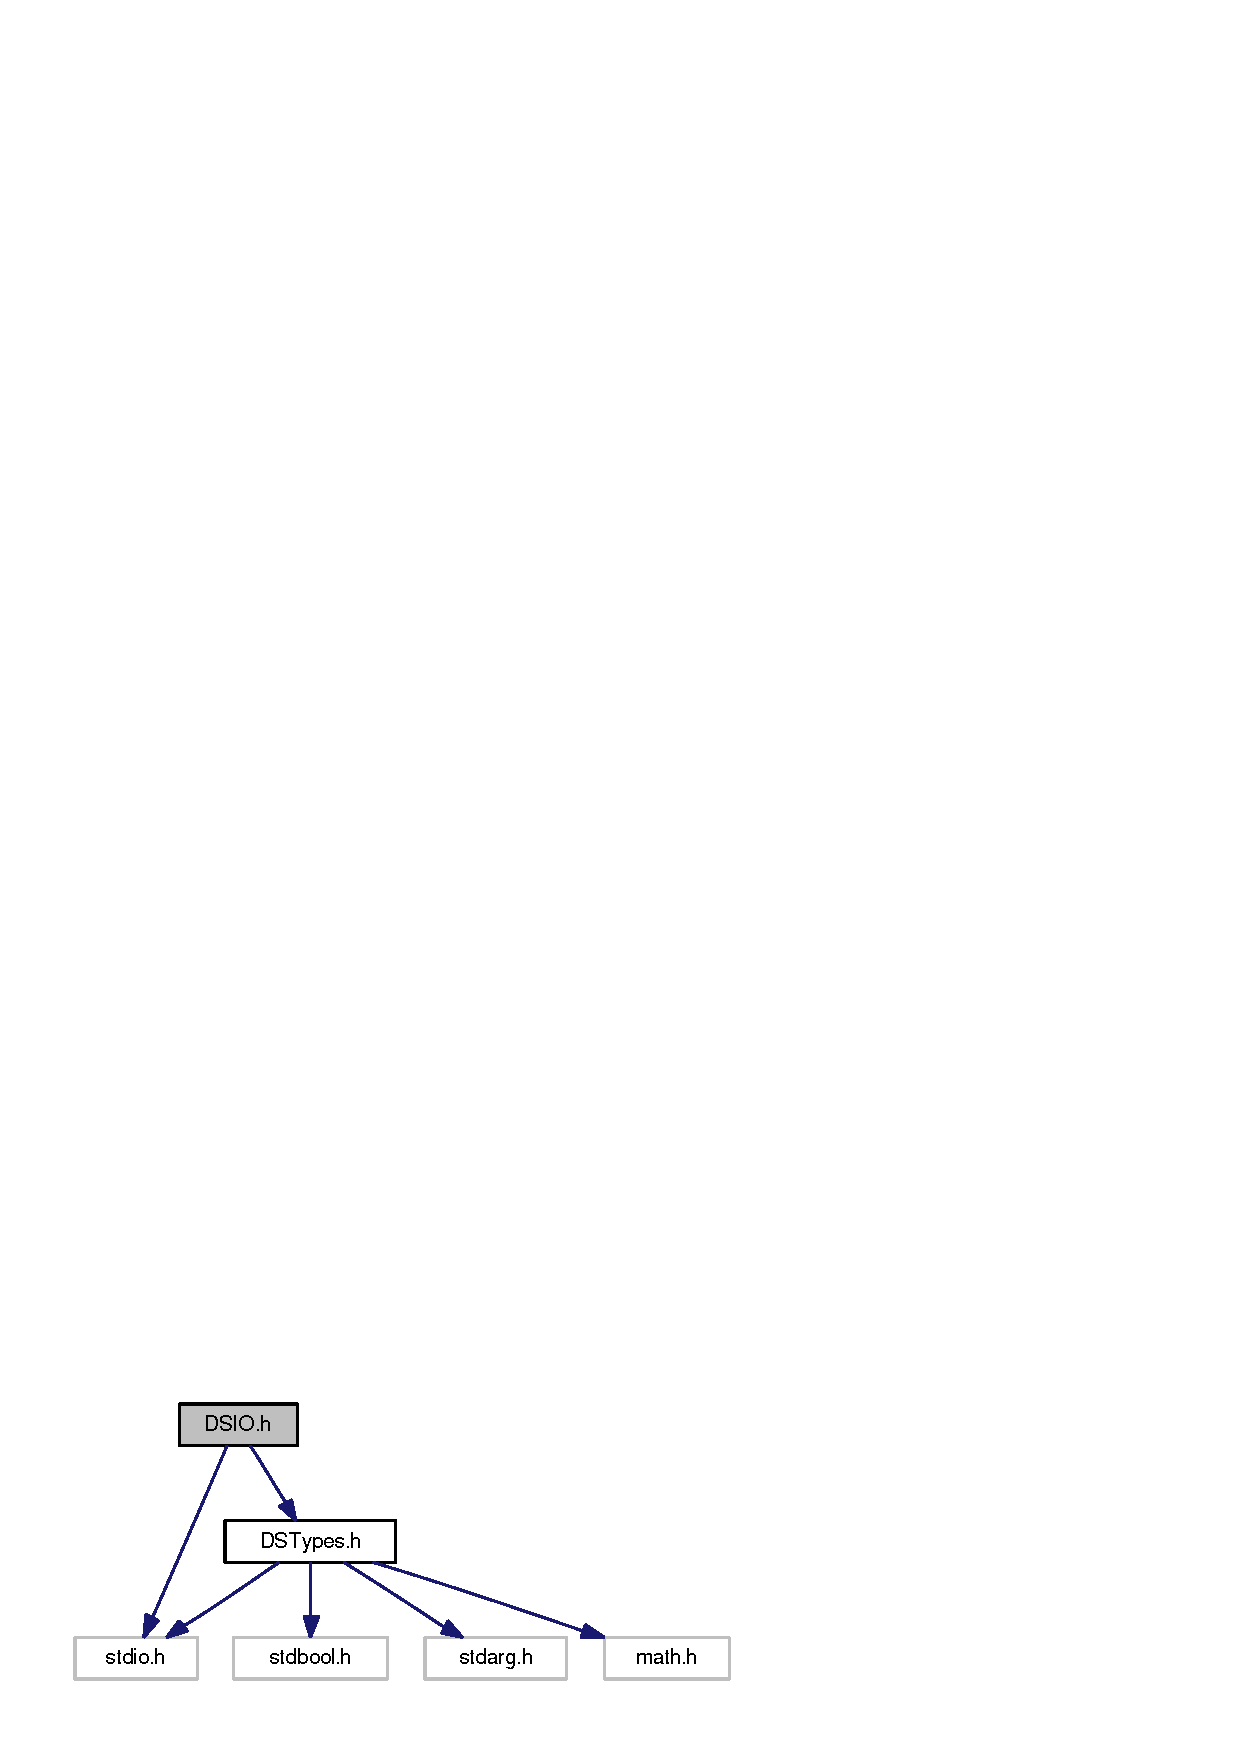
\includegraphics[width=175pt]{_d_s_i_o_8h__incl}
\end{center}
\end{figure}
This graph shows which files directly or indirectly include this file:\nopagebreak
\begin{figure}[H]
\begin{center}
\leavevmode
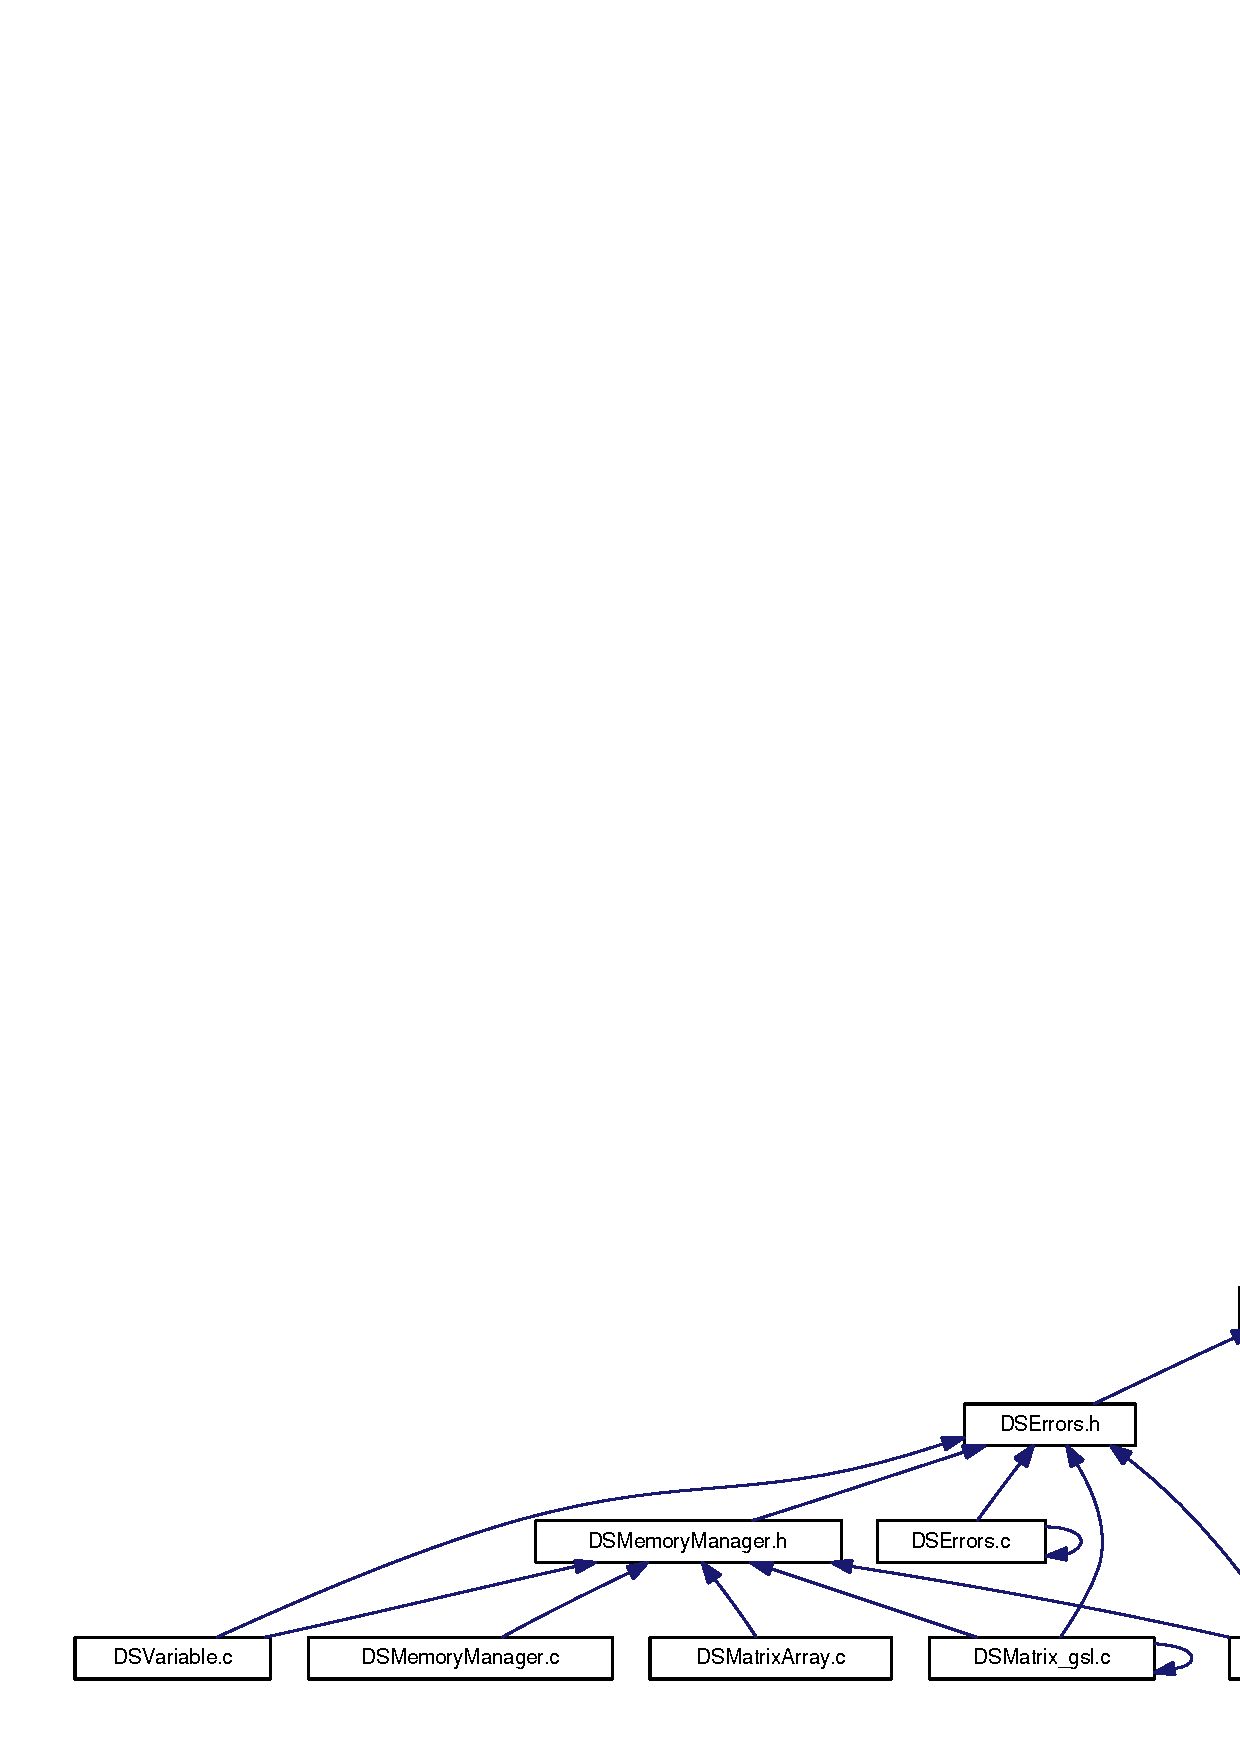
\includegraphics[width=354pt]{_d_s_i_o_8h__dep__incl}
\end{center}
\end{figure}
\subsection*{Defines}
\begin{DoxyCompactItemize}
\item 
\hypertarget{group___d_s___c_a_s_e___j_s_o_n___o_p_t_i_o_n_s_gae22b11d61deb34f2a04597b5b52e0186}{
\#define \hyperlink{group___d_s___c_a_s_e___j_s_o_n___o_p_t_i_o_n_s_gae22b11d61deb34f2a04597b5b52e0186}{DS\_\-CASE\_\-JSON\_\-NO\_\-SSYSTEM}~1}
\label{group___d_s___c_a_s_e___j_s_o_n___o_p_t_i_o_n_s_gae22b11d61deb34f2a04597b5b52e0186}

\begin{DoxyCompactList}\small\item\em Flag value indicating that the S-\/System information should not be included in the JSON string. \item\end{DoxyCompactList}\item 
\hypertarget{group___d_s___c_a_s_e___j_s_o_n___o_p_t_i_o_n_s_gaae3a87d36892fd5744ebe4ad8b111ddf}{
\#define \hyperlink{group___d_s___c_a_s_e___j_s_o_n___o_p_t_i_o_n_s_gaae3a87d36892fd5744ebe4ad8b111ddf}{DS\_\-CASE\_\-JSON\_\-NO\_\-CASE\_\-SIGNATURE}~2}
\label{group___d_s___c_a_s_e___j_s_o_n___o_p_t_i_o_n_s_gaae3a87d36892fd5744ebe4ad8b111ddf}

\begin{DoxyCompactList}\small\item\em Flag value indicating that the case signature should not be included in the JSON string. \item\end{DoxyCompactList}\item 
\hypertarget{group___d_s___c_a_s_e___j_s_o_n___o_p_t_i_o_n_s_ga43b67d5fc5384d7f11297fa0dab16a72}{
\#define \hyperlink{group___d_s___c_a_s_e___j_s_o_n___o_p_t_i_o_n_s_ga43b67d5fc5384d7f11297fa0dab16a72}{DS\_\-CASE\_\-JSON\_\-NO\_\-CONDITIONS}~4}
\label{group___d_s___c_a_s_e___j_s_o_n___o_p_t_i_o_n_s_ga43b67d5fc5384d7f11297fa0dab16a72}

\begin{DoxyCompactList}\small\item\em Flag value indicating that the conditions for validity should not be included in the JSON string. \item\end{DoxyCompactList}\item 
\hypertarget{group___d_s___s_s_y_s_t_e_m___j_s_o_n___o_p_t_i_o_n_s_gade5134b08dd7f1da683bdb3fb876cc11}{
\#define \hyperlink{group___d_s___s_s_y_s_t_e_m___j_s_o_n___o_p_t_i_o_n_s_gade5134b08dd7f1da683bdb3fb876cc11}{DS\_\-SSYSTEM\_\-JSON\_\-NO\_\-SOLUTION}~1}
\label{group___d_s___s_s_y_s_t_e_m___j_s_o_n___o_p_t_i_o_n_s_gade5134b08dd7f1da683bdb3fb876cc11}

\begin{DoxyCompactList}\small\item\em Flag value indicating that the S-\/System solution should not be included in the JSON string. \item\end{DoxyCompactList}\item 
\hypertarget{group___d_s___s_s_y_s_t_e_m___j_s_o_n___o_p_t_i_o_n_s_ga81352fdd00a529e9a2bc2be107fd7a9b}{
\#define \hyperlink{group___d_s___s_s_y_s_t_e_m___j_s_o_n___o_p_t_i_o_n_s_ga81352fdd00a529e9a2bc2be107fd7a9b}{DS\_\-SSYSTEM\_\-JSON\_\-NO\_\-SINGULAR}~2}
\label{group___d_s___s_s_y_s_t_e_m___j_s_o_n___o_p_t_i_o_n_s_ga81352fdd00a529e9a2bc2be107fd7a9b}

\begin{DoxyCompactList}\small\item\em Flag value indicating that the JSON string will not indicate if the S-\/System is singular. \item\end{DoxyCompactList}\end{DoxyCompactItemize}
\subsection*{Functions}
\begin{DoxyCompactItemize}
\item 
void \hyperlink{_d_s_i_o_8h_a71e4035e82cf614f1be280b127213ca6}{DSIOSetErrorFile} (FILE $\ast$aFile)
\begin{DoxyCompactList}\small\item\em Function to assign default error file. \item\end{DoxyCompactList}\item 
void \hyperlink{_d_s_i_o_8h_aaa699261767672e938101744e4032249}{DSIOSetPrintFunction} (int($\ast$printFunction)(const char $\ast$,...))
\begin{DoxyCompactList}\small\item\em Function to assign default printf function. \item\end{DoxyCompactList}\item 
void \hyperlink{_d_s_i_o_8h_a37a5183ebd833f0cf9bc2ed19e43fb84}{DSIOSetPostWarningFunction} (void($\ast$warningFunction)(const char $\ast$message))
\begin{DoxyCompactList}\small\item\em Function to assign default warning posting function. \item\end{DoxyCompactList}\item 
void \hyperlink{_d_s_i_o_8h_a8c9be4c3d8b1802aa5295165c3f0b861}{DSIOSetPostErrorFunction} (void($\ast$errorFunction)(const char $\ast$message))
\begin{DoxyCompactList}\small\item\em Function to assign default error posting function. \item\end{DoxyCompactList}\item 
void \hyperlink{_d_s_i_o_8h_a1fbcb57d54a5ac852484b43e317aa43f}{DSIOSetPostFatalErrorFunction} (void($\ast$fatalErrorFunction)(const char $\ast$message))
\begin{DoxyCompactList}\small\item\em Function to assign default fatal error posting function. \item\end{DoxyCompactList}\item 
void \hyperlink{_d_s_i_o_8h_a6cb102dc8b55faa48dca0c51fa0fb517}{DSIOSetCaseJSONOptions} (const DSUInteger options)
\begin{DoxyCompactList}\small\item\em Function that sets the conversion options for a \hyperlink{struct_d_s_case}{DSCase} to JSON format. \item\end{DoxyCompactList}\item 
void \hyperlink{_d_s_i_o_8h_a2a957ad88bd1a2f4d5b0ed616344c7ac}{DSIOSetSSystemJSONOptions} (const DSUInteger options)
\begin{DoxyCompactList}\small\item\em Function that sets the conversion options for a \hyperlink{struct_d_s_s_system}{DSSSystem} to JSON format. \item\end{DoxyCompactList}\item 
char $\ast$ \hyperlink{_d_s_i_o_8h_a754fa75644786b862aabc2660f191d14}{DSVariablePoolStringInJSONFormat} (const \hyperlink{struct_d_s_variable_pool}{DSVariablePool} $\ast$pool)
\begin{DoxyCompactList}\small\item\em Function to convert a \hyperlink{struct_d_s_variable_pool}{DSVariablePool} into a JSON formatted string. \item\end{DoxyCompactList}\item 
char $\ast$ \hyperlink{_d_s_i_o_8h_a6a9e23721286736288947c43461f12ae}{DSMatrixStringInJSONFormat} (const \hyperlink{struct_d_s_matrix}{DSMatrix} $\ast$matrix)
\begin{DoxyCompactList}\small\item\em Function to convert a \hyperlink{struct_d_s_matrix}{DSMatrix} into a JSON formatted string. \item\end{DoxyCompactList}\item 
char $\ast$ \hyperlink{_d_s_i_o_8h_ab8cae51e1c113fc52e1da34fffdc6f40}{DSMatrixArrayStringInJSONFormat} (const \hyperlink{struct_d_s_matrix_array}{DSMatrixArray} $\ast$array)
\begin{DoxyCompactList}\small\item\em Function to convert a \hyperlink{struct_d_s_matrix_array}{DSMatrixArray} into a JSON formatted string. \item\end{DoxyCompactList}\item 
char $\ast$ \hyperlink{_d_s_i_o_8h_a2679d81ab81c12c930cbb7a5e2791d73}{DSSSystemStringInJSONFormat} (const \hyperlink{struct_d_s_s_system}{DSSSystem} $\ast$ssys)
\begin{DoxyCompactList}\small\item\em Function to convert a \hyperlink{struct_d_s_s_system}{DSSSystem} into a JSON formatted string. \item\end{DoxyCompactList}\item 
char $\ast$ \hyperlink{_d_s_i_o_8h_a08dbac8a5ae623c94cf44bd620e46060}{DSCaseStringInJSONFormat} (const \hyperlink{struct_d_s_case}{DSCase} $\ast$aCase)
\begin{DoxyCompactList}\small\item\em Function to convert a \hyperlink{struct_d_s_case}{DSCase} into a JSON formatted string. \item\end{DoxyCompactList}\item 
\hypertarget{_d_s_i_o_8h_a5bf56bf18214f64ec10eeb8a612f3e25}{
\hyperlink{struct_d_s_variable_pool}{DSVariablePool} $\ast$ {\bfseries DSVariablePoolByParsingStringInJSONFormat} (const char $\ast$string)}
\label{_d_s_i_o_8h_a5bf56bf18214f64ec10eeb8a612f3e25}

\item 
\hypertarget{_d_s_i_o_8h_a33da47a60e8affc7aa18e3ae77fac33b}{
\hyperlink{struct_d_s_matrix}{DSMatrix} $\ast$ {\bfseries DSMatrixByParsingStringInJSONFormat} (const char $\ast$string)}
\label{_d_s_i_o_8h_a33da47a60e8affc7aa18e3ae77fac33b}

\item 
\hypertarget{_d_s_i_o_8h_a30d4cd36b9779ea2c0b5f4517ffe2dfc}{
\hyperlink{struct_d_s_matrix_array}{DSMatrixArray} $\ast$ {\bfseries DSMatrixArrayByParsingStringInJSONFormat} (const char $\ast$string)}
\label{_d_s_i_o_8h_a30d4cd36b9779ea2c0b5f4517ffe2dfc}

\item 
\hypertarget{_d_s_i_o_8h_a13aa821864b0a082f7d77e4aaf08985d}{
\hyperlink{struct_d_s_s_system}{DSSSystem} $\ast$ {\bfseries DSSSystemByParsingStringInJSONFormat} (const char $\ast$string)}
\label{_d_s_i_o_8h_a13aa821864b0a082f7d77e4aaf08985d}

\item 
\hypertarget{_d_s_i_o_8h_a858a6748dbf86dbc5cd5d31146165b15}{
\hyperlink{struct_d_s_case}{DSCase} $\ast$ {\bfseries DSCaseByParsingStringInJSONFormat} (const char $\ast$string)}
\label{_d_s_i_o_8h_a858a6748dbf86dbc5cd5d31146165b15}

\end{DoxyCompactItemize}
\subsection*{Variables}
\begin{DoxyCompactItemize}
\item 
int($\ast$ \hyperlink{_d_s_i_o_8h_a01ab8215975bf8e2086ad342cfa6be26}{DSPrintf} )(const char $\ast$,...)
\begin{DoxyCompactList}\small\item\em Pointer to a function determining how messages are printed. \item\end{DoxyCompactList}\item 
void($\ast$ \hyperlink{_d_s_i_o_8h_af12cf032b729ba022698fadaccfea33d}{DSPostWarning} )(const char $\ast$message)
\begin{DoxyCompactList}\small\item\em Pointer to a function determining how warning are handled. \item\end{DoxyCompactList}\item 
void($\ast$ \hyperlink{_d_s_i_o_8h_a40c3f80fe9e5002beb7d258e4f89c8d2}{DSPostError} )(const char $\ast$message)
\begin{DoxyCompactList}\small\item\em Pointer to a function determining how errors are handled. \item\end{DoxyCompactList}\item 
void($\ast$ \hyperlink{_d_s_i_o_8h_a41b7b42028f3c25f17ca479154c7492d}{DSPostFatalError} )(const char $\ast$message)
\begin{DoxyCompactList}\small\item\em Pointer to a function determining how fatal errors are handled. \item\end{DoxyCompactList}\item 
FILE $\ast$ \hyperlink{_d_s_i_o_8h_af8405bae84409f99d5fa564ebaff4c91}{DSIOErrorFile}
\begin{DoxyCompactList}\small\item\em FILE pointer used for default error/warning printing. \item\end{DoxyCompactList}\end{DoxyCompactItemize}


\subsection{Detailed Description}
Header file with standard input and output functions. Copyright (C) 2011 Jason Lomnitz.\par
\par


This file is part of the Design Space Toolbox V2 (C Library).

The Design Space Toolbox V2 is free software: you can redistribute it and/or modify it under the terms of the GNU General Public License as published by the Free Software Foundation, either version 3 of the License, or (at your option) any later version.

The Design Space Toolbox V2 is distributed in the hope that it will be useful, but WITHOUT ANY WARRANTY; without even the implied warranty of MERCHANTABILITY or FITNESS FOR A PARTICULAR PURPOSE. See the GNU General Public License for more details.

You should have received a copy of the GNU General Public License along with the Design Space Toolbox. If not, see $<$\href{http://www.gnu.org/licenses/}{\tt http://www.gnu.org/licenses/}$>$.

\begin{DoxyAuthor}{Author}
Jason Lomnitz. 
\end{DoxyAuthor}
\begin{DoxyDate}{Date}
2011
\end{DoxyDate}
\begin{Desc}
\item[\hyperlink{todo__todo000002}{Todo}]Define standard input and output file formats. 

Define criteria for warnings, errors and fatal errors.\end{Desc}


\subsection{Function Documentation}
\hypertarget{_d_s_i_o_8h_a08dbac8a5ae623c94cf44bd620e46060}{
\index{DSIO.h@{DSIO.h}!DSCaseStringInJSONFormat@{DSCaseStringInJSONFormat}}
\index{DSCaseStringInJSONFormat@{DSCaseStringInJSONFormat}!DSIO.h@{DSIO.h}}
\subsubsection[{DSCaseStringInJSONFormat}]{\setlength{\rightskip}{0pt plus 5cm}char$\ast$ DSCaseStringInJSONFormat (const {\bf DSCase} $\ast$ {\em aCase})}}
\label{_d_s_i_o_8h_a08dbac8a5ae623c94cf44bd620e46060}


Function to convert a \hyperlink{struct_d_s_case}{DSCase} into a JSON formatted string. 

This function is used to convert a \hyperlink{struct_d_s_case}{DSCase} into a JSON object. The \hyperlink{struct_d_s_case}{DSCase} is represented with a set of objects, where each object is a field of the \hyperlink{struct_d_s_case}{DSCase} object. The default behavior exports all of the fields, this behavior can be overwritten by changing the \hyperlink{struct_d_s_case}{DSCase} conversion options.


\begin{DoxyParams}{Parameters}
\item[{\em aCase}]A \hyperlink{struct_d_s_case}{DSCase} that will be used to create the JSON object.\end{DoxyParams}
\begin{DoxyReturn}{Returns}
A C string with the JSON formatted data. If NULL, the conversion failed.
\end{DoxyReturn}
\begin{DoxySeeAlso}{See also}
\hyperlink{_d_s_i_o_8c_a6cb102dc8b55faa48dca0c51fa0fb517}{DSIOSetCaseJSONOptions()} 
\end{DoxySeeAlso}
\hypertarget{_d_s_i_o_8h_a6cb102dc8b55faa48dca0c51fa0fb517}{
\index{DSIO.h@{DSIO.h}!DSIOSetCaseJSONOptions@{DSIOSetCaseJSONOptions}}
\index{DSIOSetCaseJSONOptions@{DSIOSetCaseJSONOptions}!DSIO.h@{DSIO.h}}
\subsubsection[{DSIOSetCaseJSONOptions}]{\setlength{\rightskip}{0pt plus 5cm}void DSIOSetCaseJSONOptions (const DSUInteger {\em options})}}
\label{_d_s_i_o_8h_a6cb102dc8b55faa48dca0c51fa0fb517}


Function that sets the conversion options for a \hyperlink{struct_d_s_case}{DSCase} to JSON format. 

This function is used to overwrite the default export behavior of the \hyperlink{struct_d_s_case}{DSCase} object. The default behavior converts all of the data fields of the \hyperlink{struct_d_s_case}{DSCase} into a JSON format, these options can be changed so the JSON conversion only includes some fields, such as excluding the conditions, excluding the S-\/System, etc.


\begin{DoxyParams}{Parameters}
\item[{\em options}]A DSUInteger with the option flags, as specified by the \hyperlink{struct_d_s_case}{DSCase} options.\end{DoxyParams}
\begin{DoxySeeAlso}{See also}
\hyperlink{group___d_s___c_a_s_e___j_s_o_n___o_p_t_i_o_n_s}{Options for JSON conversion of DSCase object.} 
\end{DoxySeeAlso}
\hypertarget{_d_s_i_o_8h_a71e4035e82cf614f1be280b127213ca6}{
\index{DSIO.h@{DSIO.h}!DSIOSetErrorFile@{DSIOSetErrorFile}}
\index{DSIOSetErrorFile@{DSIOSetErrorFile}!DSIO.h@{DSIO.h}}
\subsubsection[{DSIOSetErrorFile}]{\setlength{\rightskip}{0pt plus 5cm}void DSIOSetErrorFile (FILE $\ast$ {\em aFile})}}
\label{_d_s_i_o_8h_a71e4035e82cf614f1be280b127213ca6}


Function to assign default error file. 

This function is used to assign the default error file, DSIOErrorFile. Changing the error file should be done via this function, as it circumvents potential problems associated with dynamic linking.


\begin{DoxyParams}{Parameters}
\item[{\em aFile}]A FILE $\ast$ that will be used to write error messages when the default error posting mechanism is used.\end{DoxyParams}
\begin{DoxySeeAlso}{See also}
\hyperlink{_d_s_i_o_8h_a37a5183ebd833f0cf9bc2ed19e43fb84}{DSIOSetPostWarningFunction} 

\hyperlink{_d_s_i_o_8h_a8c9be4c3d8b1802aa5295165c3f0b861}{DSIOSetPostErrorFunction} 

\hyperlink{_d_s_i_o_8h_a1fbcb57d54a5ac852484b43e317aa43f}{DSIOSetPostFatalErrorFunction} 

\hyperlink{_d_s_errors_8h_a09b28eb2b01986855910ca97dfe91144}{DSError} 
\end{DoxySeeAlso}
\hypertarget{_d_s_i_o_8h_a8c9be4c3d8b1802aa5295165c3f0b861}{
\index{DSIO.h@{DSIO.h}!DSIOSetPostErrorFunction@{DSIOSetPostErrorFunction}}
\index{DSIOSetPostErrorFunction@{DSIOSetPostErrorFunction}!DSIO.h@{DSIO.h}}
\subsubsection[{DSIOSetPostErrorFunction}]{\setlength{\rightskip}{0pt plus 5cm}void DSIOSetPostErrorFunction (void($\ast$)(const char $\ast$message) {\em errorFunction})}}
\label{_d_s_i_o_8h_a8c9be4c3d8b1802aa5295165c3f0b861}


Function to assign default error posting function. 

This function is used to assign the function that handles the errors generated from the design space toolbox. Internally, it assigns the global variable DSPostError which points to a function.


\begin{DoxyParams}{Parameters}
\item[{\em errorFunction}]A pointer to a function of the form void function(const char $\ast$). If NULL, default behavior is restored. \end{DoxyParams}
\hypertarget{_d_s_i_o_8h_a1fbcb57d54a5ac852484b43e317aa43f}{
\index{DSIO.h@{DSIO.h}!DSIOSetPostFatalErrorFunction@{DSIOSetPostFatalErrorFunction}}
\index{DSIOSetPostFatalErrorFunction@{DSIOSetPostFatalErrorFunction}!DSIO.h@{DSIO.h}}
\subsubsection[{DSIOSetPostFatalErrorFunction}]{\setlength{\rightskip}{0pt plus 5cm}void DSIOSetPostFatalErrorFunction (void($\ast$)(const char $\ast$message) {\em fatalErrorFunction})}}
\label{_d_s_i_o_8h_a1fbcb57d54a5ac852484b43e317aa43f}


Function to assign default fatal error posting function. 

This function is used to assign the function that handles the fatal errors generated from the design space toolbox. Internally, it assigns the global variable DSPostFatalError which points to a function.


\begin{DoxyParams}{Parameters}
\item[{\em errorFunction}]A pointer to a function of the form void function(const char $\ast$). If NULL, default behavior is restored. \end{DoxyParams}
\hypertarget{_d_s_i_o_8h_a37a5183ebd833f0cf9bc2ed19e43fb84}{
\index{DSIO.h@{DSIO.h}!DSIOSetPostWarningFunction@{DSIOSetPostWarningFunction}}
\index{DSIOSetPostWarningFunction@{DSIOSetPostWarningFunction}!DSIO.h@{DSIO.h}}
\subsubsection[{DSIOSetPostWarningFunction}]{\setlength{\rightskip}{0pt plus 5cm}void DSIOSetPostWarningFunction (void($\ast$)(const char $\ast$message) {\em warningFunction})}}
\label{_d_s_i_o_8h_a37a5183ebd833f0cf9bc2ed19e43fb84}


Function to assign default warning posting function. 

This function is used to assign the function that handles the warnings generated from the design space toolbox. Internally, it assigns the global variable DSPostWarning which points to a function.


\begin{DoxyParams}{Parameters}
\item[{\em warningFunction}]A pointer to a function of the form void function(const char $\ast$). If NULL, default behavior is restored. \end{DoxyParams}
\hypertarget{_d_s_i_o_8h_aaa699261767672e938101744e4032249}{
\index{DSIO.h@{DSIO.h}!DSIOSetPrintFunction@{DSIOSetPrintFunction}}
\index{DSIOSetPrintFunction@{DSIOSetPrintFunction}!DSIO.h@{DSIO.h}}
\subsubsection[{DSIOSetPrintFunction}]{\setlength{\rightskip}{0pt plus 5cm}void DSIOSetPrintFunction (int($\ast$)(const char $\ast$,...) {\em printFunction})}}
\label{_d_s_i_o_8h_aaa699261767672e938101744e4032249}


Function to assign default printf function. 

This function is used to assign the formated print function, DSPrintf. This function assigns the DSPrintf pointer to the function that should be used to print formatted strings. This function MUST be used to avoid problems relating to dynamic linking; by using this function the global variable DSPrintf is loaded into memory prior to changing its value.


\begin{DoxyParams}{Parameters}
\item[{\em printFunction}]A pointer to a function of the form int function(const char $\ast$, ...). If NULL, default behavior is restored. \end{DoxyParams}
\hypertarget{_d_s_i_o_8h_a2a957ad88bd1a2f4d5b0ed616344c7ac}{
\index{DSIO.h@{DSIO.h}!DSIOSetSSystemJSONOptions@{DSIOSetSSystemJSONOptions}}
\index{DSIOSetSSystemJSONOptions@{DSIOSetSSystemJSONOptions}!DSIO.h@{DSIO.h}}
\subsubsection[{DSIOSetSSystemJSONOptions}]{\setlength{\rightskip}{0pt plus 5cm}void DSIOSetSSystemJSONOptions (const DSUInteger {\em options})}}
\label{_d_s_i_o_8h_a2a957ad88bd1a2f4d5b0ed616344c7ac}


Function that sets the conversion options for a \hyperlink{struct_d_s_s_system}{DSSSystem} to JSON format. 

This function is used to overwrite the default export behavior of the \hyperlink{struct_d_s_s_system}{DSSSystem} object. The default behavior converts all of the data fields of the S-\/System into a JSON format, these options can be changed so the JSON conversion only includes some fields, such as excluding the solution.


\begin{DoxyParams}{Parameters}
\item[{\em options}]A DSUInteger with the option flags, as specified by the \hyperlink{struct_d_s_s_system}{DSSSystem} options.\end{DoxyParams}
\begin{DoxySeeAlso}{See also}
\hyperlink{group___d_s___s_s_y_s_t_e_m___j_s_o_n___o_p_t_i_o_n_s}{Options for JSON conversion of DSSSystem object.} 
\end{DoxySeeAlso}
\hypertarget{_d_s_i_o_8h_ab8cae51e1c113fc52e1da34fffdc6f40}{
\index{DSIO.h@{DSIO.h}!DSMatrixArrayStringInJSONFormat@{DSMatrixArrayStringInJSONFormat}}
\index{DSMatrixArrayStringInJSONFormat@{DSMatrixArrayStringInJSONFormat}!DSIO.h@{DSIO.h}}
\subsubsection[{DSMatrixArrayStringInJSONFormat}]{\setlength{\rightskip}{0pt plus 5cm}char$\ast$ DSMatrixArrayStringInJSONFormat (const {\bf DSMatrixArray} $\ast$ {\em array})}}
\label{_d_s_i_o_8h_ab8cae51e1c113fc52e1da34fffdc6f40}


Function to convert a \hyperlink{struct_d_s_matrix_array}{DSMatrixArray} into a JSON formatted string. 

This function is used to convert a \hyperlink{struct_d_s_matrix}{DSMatrix} into a JSON object. The matrix array is stored as an array of objects, where each object is a \hyperlink{struct_d_s_matrix}{DSMatrix}. The order of the \hyperlink{struct_d_s_matrix}{DSMatrix} object in the array represent the order of matrices in the matrix array.


\begin{DoxyParams}{Parameters}
\item[{\em array}]A \hyperlink{struct_d_s_matrix_array}{DSMatrixArray} that will be used to create the JSON object.\end{DoxyParams}
\begin{DoxyReturn}{Returns}
A C string with the JSON formatted data. If NULL, the conversion failed. 
\end{DoxyReturn}
\hypertarget{_d_s_i_o_8h_a6a9e23721286736288947c43461f12ae}{
\index{DSIO.h@{DSIO.h}!DSMatrixStringInJSONFormat@{DSMatrixStringInJSONFormat}}
\index{DSMatrixStringInJSONFormat@{DSMatrixStringInJSONFormat}!DSIO.h@{DSIO.h}}
\subsubsection[{DSMatrixStringInJSONFormat}]{\setlength{\rightskip}{0pt plus 5cm}char$\ast$ DSMatrixStringInJSONFormat (const {\bf DSMatrix} $\ast$ {\em matrix})}}
\label{_d_s_i_o_8h_a6a9e23721286736288947c43461f12ae}


Function to convert a \hyperlink{struct_d_s_matrix}{DSMatrix} into a JSON formatted string. 

This function is used to convert a \hyperlink{struct_d_s_matrix}{DSMatrix} into a JSON object. The matrix is stored as an array of arrays. The array of arrays represents the rows of the matrix, whereas the arrays of value are the values at the columns for a particular row.


\begin{DoxyParams}{Parameters}
\item[{\em matrix}]A \hyperlink{struct_d_s_matrix}{DSMatrix} that will be used to create the JSON object.\end{DoxyParams}
\begin{DoxyReturn}{Returns}
A C string with the JSON formatted data. If NULL, the conversion failed. 
\end{DoxyReturn}
\hypertarget{_d_s_i_o_8h_a2679d81ab81c12c930cbb7a5e2791d73}{
\index{DSIO.h@{DSIO.h}!DSSSystemStringInJSONFormat@{DSSSystemStringInJSONFormat}}
\index{DSSSystemStringInJSONFormat@{DSSSystemStringInJSONFormat}!DSIO.h@{DSIO.h}}
\subsubsection[{DSSSystemStringInJSONFormat}]{\setlength{\rightskip}{0pt plus 5cm}char$\ast$ DSSSystemStringInJSONFormat (const {\bf DSSSystem} $\ast$ {\em ssys})}}
\label{_d_s_i_o_8h_a2679d81ab81c12c930cbb7a5e2791d73}


Function to convert a \hyperlink{struct_d_s_s_system}{DSSSystem} into a JSON formatted string. 

This function is used to convert a \hyperlink{struct_d_s_s_system}{DSSSystem} into a JSON object. The S-\/System as a set of objects, where each object represents each of the fields of the \hyperlink{struct_d_s_s_system}{DSSSystem}. The default behavior exports all of the fields, this behavior can be overwritten by changing the S-\/System conversion options.


\begin{DoxyParams}{Parameters}
\item[{\em ssys}]A \hyperlink{struct_d_s_s_system}{DSSSystem} that will be used to create the JSON object.\end{DoxyParams}
\begin{DoxyReturn}{Returns}
A C string with the JSON formatted data. If NULL, the conversion failed.
\end{DoxyReturn}
\begin{DoxySeeAlso}{See also}
\hyperlink{_d_s_i_o_8c_a2a957ad88bd1a2f4d5b0ed616344c7ac}{DSIOSetSSystemJSONOptions()} 
\end{DoxySeeAlso}
\hypertarget{_d_s_i_o_8h_a754fa75644786b862aabc2660f191d14}{
\index{DSIO.h@{DSIO.h}!DSVariablePoolStringInJSONFormat@{DSVariablePoolStringInJSONFormat}}
\index{DSVariablePoolStringInJSONFormat@{DSVariablePoolStringInJSONFormat}!DSIO.h@{DSIO.h}}
\subsubsection[{DSVariablePoolStringInJSONFormat}]{\setlength{\rightskip}{0pt plus 5cm}char$\ast$ DSVariablePoolStringInJSONFormat (const {\bf DSVariablePool} $\ast$ {\em pool})}}
\label{_d_s_i_o_8h_a754fa75644786b862aabc2660f191d14}


Function to convert a \hyperlink{struct_d_s_variable_pool}{DSVariablePool} into a JSON formatted string. 

This function is used to convert a \hyperlink{struct_d_s_variable_pool}{DSVariablePool} into a JSON object. The variables of the variable pool are stored as pairs of a string and value.


\begin{DoxyParams}{Parameters}
\item[{\em pool}]A \hyperlink{struct_d_s_variable_pool}{DSVariablePool} that will be used to create the JSON object.\end{DoxyParams}
\begin{DoxyReturn}{Returns}
A C string with the JSON formatted data. If NULL, the conversion failed. 
\end{DoxyReturn}


\subsection{Variable Documentation}
\hypertarget{_d_s_i_o_8h_af8405bae84409f99d5fa564ebaff4c91}{
\index{DSIO.h@{DSIO.h}!DSIOErrorFile@{DSIOErrorFile}}
\index{DSIOErrorFile@{DSIOErrorFile}!DSIO.h@{DSIO.h}}
\subsubsection[{DSIOErrorFile}]{\setlength{\rightskip}{0pt plus 5cm}FILE$\ast$ {\bf DSIOErrorFile}}}
\label{_d_s_i_o_8h_af8405bae84409f99d5fa564ebaff4c91}


FILE pointer used for default error/warning printing. 

This pointer to a FILE tells the error handling system which FILE to print the error messages to. If this pointer is NULL, then the system sets it to the stderr file. This variable is only used internally with the default behavior of DSErrorFunction. To change the error file, the function DSIOSetErrorFile should be used in order to avoid errors caused by dynamic linking. These errors involve changing the value of a global variable that has not yet been loaded by the linker.

\begin{DoxySeeAlso}{See also}
\hyperlink{_d_s_i_o_8h_a71e4035e82cf614f1be280b127213ca6}{DSIOSetErrorFile} 

\hyperlink{_d_s_errors_8h_a363f9c264b785ec509da1b11af9ae314}{DSErrorFunction} 
\end{DoxySeeAlso}
\hypertarget{_d_s_i_o_8h_a40c3f80fe9e5002beb7d258e4f89c8d2}{
\index{DSIO.h@{DSIO.h}!DSPostError@{DSPostError}}
\index{DSPostError@{DSPostError}!DSIO.h@{DSIO.h}}
\subsubsection[{DSPostError}]{\setlength{\rightskip}{0pt plus 5cm}void($\ast$ {\bf DSPostError})(const char $\ast$message)}}
\label{_d_s_i_o_8h_a40c3f80fe9e5002beb7d258e4f89c8d2}


Pointer to a function determining how errors are handled. 

This pointer to a function is used by DSErrorFunction to post erros. This pointer should be used to allow better integration of errors in programs that make use of the DesignSpaceToolbox. The function takes one argument, a constant C string with the error message. To change the function used, the function DSIOSetPostErrorFunction should be used. This is to avoid errors caused by dynamic linking. These errors involve changing the value of a global variable that has not yet been loaded by the linker.

\begin{DoxySeeAlso}{See also}
\hyperlink{_d_s_i_o_8h_a8c9be4c3d8b1802aa5295165c3f0b861}{DSIOSetPostErrorFunction} 
\end{DoxySeeAlso}
\hypertarget{_d_s_i_o_8h_a41b7b42028f3c25f17ca479154c7492d}{
\index{DSIO.h@{DSIO.h}!DSPostFatalError@{DSPostFatalError}}
\index{DSPostFatalError@{DSPostFatalError}!DSIO.h@{DSIO.h}}
\subsubsection[{DSPostFatalError}]{\setlength{\rightskip}{0pt plus 5cm}void($\ast$ {\bf DSPostFatalError})(const char $\ast$message)}}
\label{_d_s_i_o_8h_a41b7b42028f3c25f17ca479154c7492d}


Pointer to a function determining how fatal errors are handled. 

This pointer to a function is used by DSErrorFunction to post fatal erros. This pointer should be used to allow better integration of errors in programs that make use of the DesignSpaceToolbox. The function takes one argument, a constant C string with the error message. To change the function used, the function DSIOSetPostFatalErrorFunction should be used. This is to avoid errors caused by dynamic linking. These errors involve changing the value of a global variable that has not yet been loaded by the linker.

\begin{DoxySeeAlso}{See also}
\hyperlink{_d_s_i_o_8h_a8c9be4c3d8b1802aa5295165c3f0b861}{DSIOSetPostErrorFunction} 
\end{DoxySeeAlso}
\hypertarget{_d_s_i_o_8h_af12cf032b729ba022698fadaccfea33d}{
\index{DSIO.h@{DSIO.h}!DSPostWarning@{DSPostWarning}}
\index{DSPostWarning@{DSPostWarning}!DSIO.h@{DSIO.h}}
\subsubsection[{DSPostWarning}]{\setlength{\rightskip}{0pt plus 5cm}void($\ast$ {\bf DSPostWarning})(const char $\ast$message)}}
\label{_d_s_i_o_8h_af12cf032b729ba022698fadaccfea33d}


Pointer to a function determining how warning are handled. 

This pointer to a function is used by DSErrorFunction to post warnings. This pointer should be used to allow better integration of warnings in programs that make use of the DesignSpaceToolbox. The function takes one argument, a constant C string with the warning message. To change the function used, the function DSIOSetPostWarningFunction should be used. This is to avoid errors caused by dynamic linking. These errors involve changing the value of a global variable that has not yet been loaded by the linker.

\begin{DoxySeeAlso}{See also}
\hyperlink{_d_s_i_o_8h_a37a5183ebd833f0cf9bc2ed19e43fb84}{DSIOSetPostWarningFunction} 
\end{DoxySeeAlso}
\hypertarget{_d_s_i_o_8h_a01ab8215975bf8e2086ad342cfa6be26}{
\index{DSIO.h@{DSIO.h}!DSPrintf@{DSPrintf}}
\index{DSPrintf@{DSPrintf}!DSIO.h@{DSIO.h}}
\subsubsection[{DSPrintf}]{\setlength{\rightskip}{0pt plus 5cm}int($\ast$ {\bf DSPrintf})(const char $\ast$,...)}}
\label{_d_s_i_o_8h_a01ab8215975bf8e2086ad342cfa6be26}


Pointer to a function determining how messages are printed. 

This pointer to a function tells the error handling system which function to call with the error messages. If this pointer is NULL, the design space toolbox should have a default printing format, using printf to stdout. This pointer is intended to be used to override default behavior to be override. An example could be by using the mexPrintf function in matlab.

\begin{DoxySeeAlso}{See also}
\hyperlink{_d_s_i_o_8h_aaa699261767672e938101744e4032249}{DSIOSetPrintFunction} 
\end{DoxySeeAlso}

\include{_d_s_matrix_8h}
\hypertarget{_d_s_matrix__gsl_8c}{
\section{DSMatrix\_\-gsl.c File Reference}
\label{_d_s_matrix__gsl_8c}\index{DSMatrix\_\-gsl.c@{DSMatrix\_\-gsl.c}}
}


Implementation file with functions for dealing with matrices using the GNU Scientific Library (gsl).  


{\ttfamily \#include $<$time.h$>$}\par
{\ttfamily \#include $<$stdarg.h$>$}\par
{\ttfamily \#include $<$string.h$>$}\par
{\ttfamily \#include $<$unistd.h$>$}\par
{\ttfamily \#include $<$gsl/gsl\_\-linalg.h$>$}\par
{\ttfamily \#include $<$gsl/gsl\_\-blas.h$>$}\par
{\ttfamily \#include \char`\"{}DSMatrix.h\char`\"{}}\par
{\ttfamily \#include \char`\"{}DSErrors.h\char`\"{}}\par
{\ttfamily \#include \char`\"{}DSMemoryManager.h\char`\"{}}\par
{\ttfamily \#include \char`\"{}DSMatrixArray.h\char`\"{}}\par
{\ttfamily \#include \char`\"{}DSMatrixTokenizer.h\char`\"{}}\par
{\ttfamily \#include \char`\"{}DSTypes.h\char`\"{}}\par
Include dependency graph for DSMatrix\_\-gsl.c:\nopagebreak
\begin{figure}[H]
\begin{center}
\leavevmode
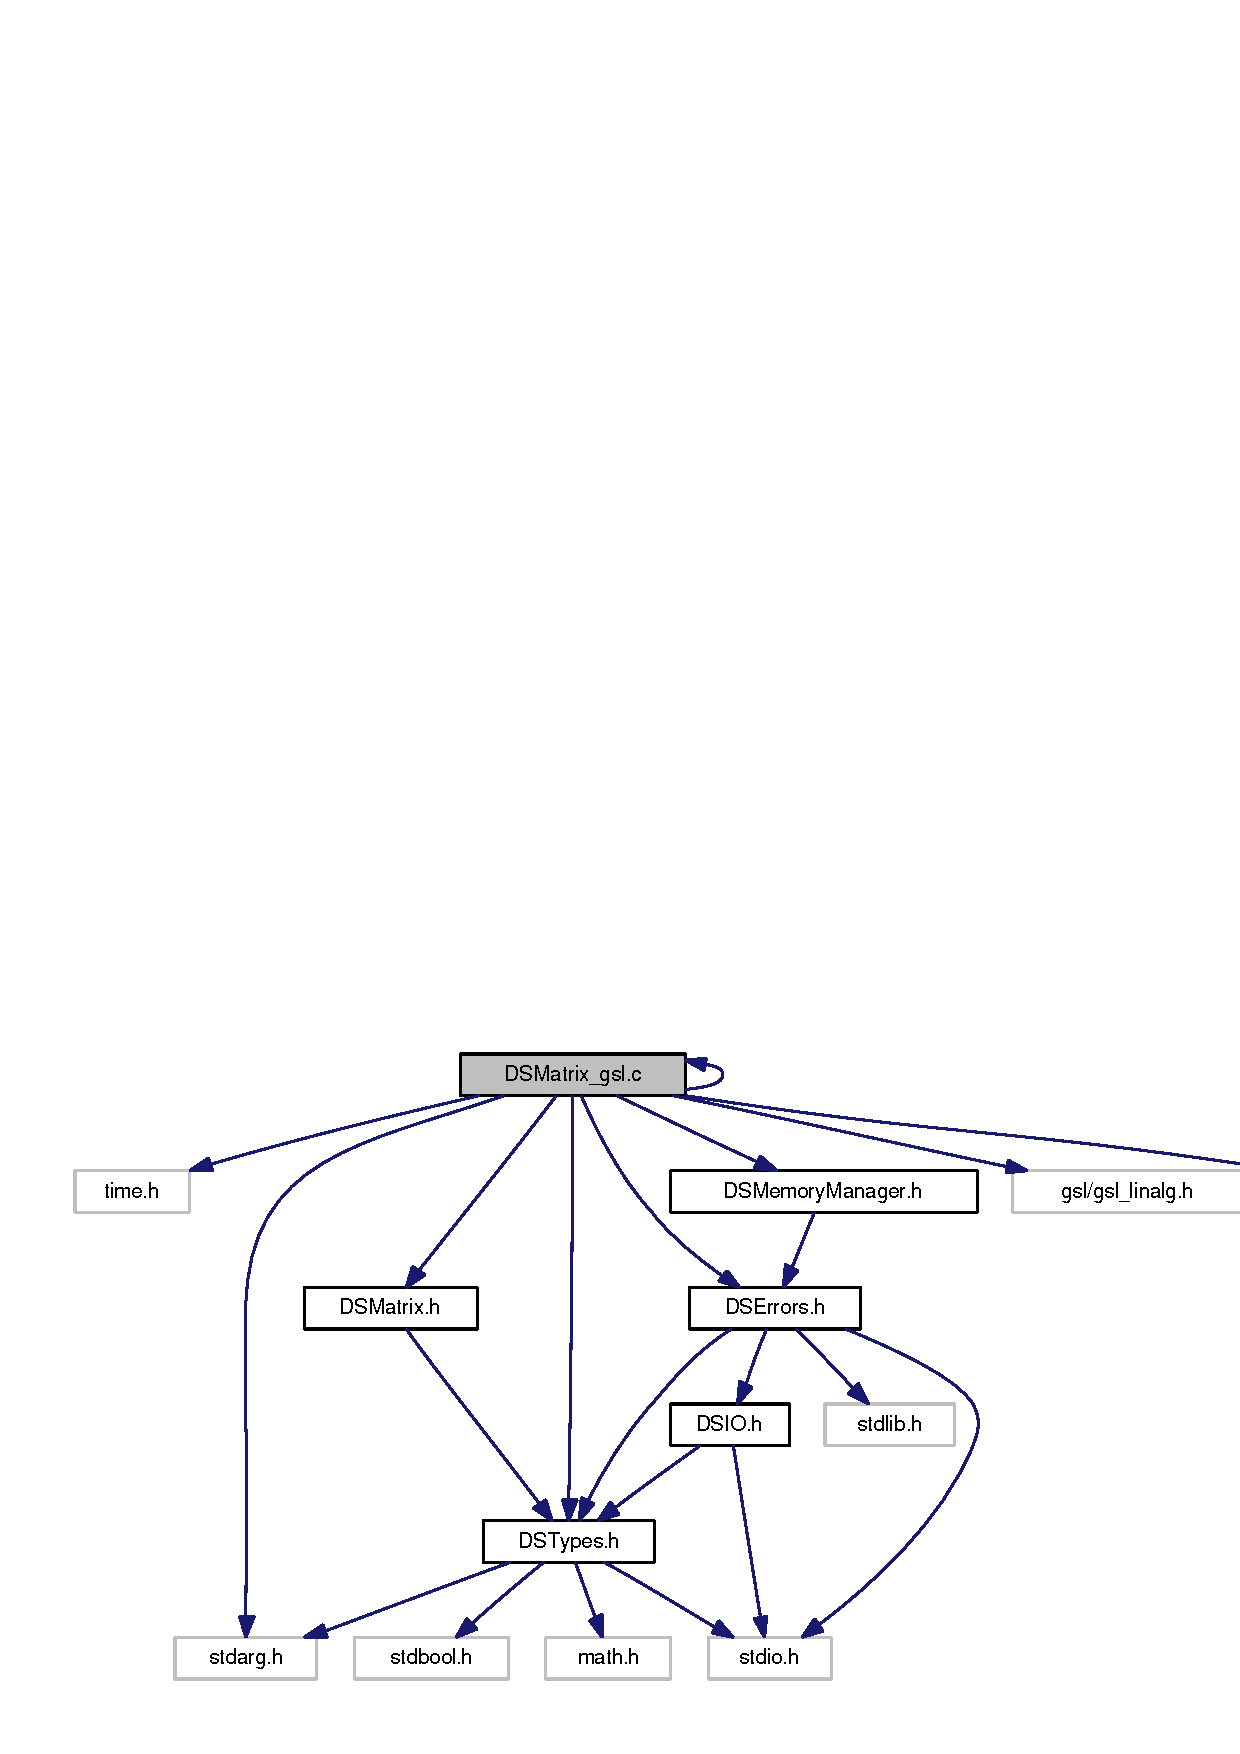
\includegraphics[width=358pt]{_d_s_matrix__gsl_8c__incl}
\end{center}
\end{figure}
This graph shows which files directly or indirectly include this file:\nopagebreak
\begin{figure}[H]
\begin{center}
\leavevmode
\includegraphics[width=81pt]{_d_s_matrix__gsl_8c__dep__incl}
\end{center}
\end{figure}
\subsection*{Defines}
\begin{DoxyCompactItemize}
\item 
\hypertarget{_d_s_matrix__gsl_8c_ad6dbca80a166e990b667278effb31731}{
\#define {\bfseries DSMatrixSetRows}(x, y)~((x)-\/$>$rows = (y))}
\label{_d_s_matrix__gsl_8c_ad6dbca80a166e990b667278effb31731}

\item 
\hypertarget{_d_s_matrix__gsl_8c_aa1051e84e33639a1cd4b276695bfe52e}{
\#define {\bfseries DSMatrixSetColumns}(x, y)~((x)-\/$>$columns = (y))}
\label{_d_s_matrix__gsl_8c_aa1051e84e33639a1cd4b276695bfe52e}

\end{DoxyCompactItemize}
\subsection*{Functions}
\begin{DoxyCompactItemize}
\item 
\hyperlink{struct_d_s_matrix}{DSMatrix} $\ast$ \hyperlink{_d_s_matrix__gsl_8c_abfe7884de06da66ce4bc46c7048d4e49}{DSMatrixAlloc} (const DSUInteger rows, const DSUInteger columns)
\begin{DoxyCompactList}\small\item\em Memory allocation for a \hyperlink{struct_d_s_matrix}{DSMatrix} using malloc. \item\end{DoxyCompactList}\item 
\hyperlink{struct_d_s_matrix}{DSMatrix} $\ast$ \hyperlink{_d_s_matrix__gsl_8c_a1b228ecc7be521c40160173fc1cecea2}{DSMatrixCalloc} (const DSUInteger rows, const DSUInteger columns)
\begin{DoxyCompactList}\small\item\em Memory allocation for a \hyperlink{struct_d_s_matrix}{DSMatrix} using calloc. \item\end{DoxyCompactList}\item 
\hyperlink{struct_d_s_matrix}{DSMatrix} $\ast$ \hyperlink{_d_s_matrix__gsl_8c_a6d0f0f74bdd85829ba07dd33f51cfa11}{DSMatrixCopy} (const \hyperlink{struct_d_s_matrix}{DSMatrix} $\ast$original)
\begin{DoxyCompactList}\small\item\em Copies a \hyperlink{struct_d_s_matrix}{DSMatrix}. \item\end{DoxyCompactList}\item 
void \hyperlink{_d_s_matrix__gsl_8c_ae5fc6bceef5e7e9e2c6300a86bdfb5fc}{DSMatrixFree} (\hyperlink{struct_d_s_matrix}{DSMatrix} $\ast$matrix)
\begin{DoxyCompactList}\small\item\em Freeing memory for \hyperlink{struct_d_s_matrix}{DSMatrix}. \item\end{DoxyCompactList}\item 
\hyperlink{struct_d_s_matrix}{DSMatrix} $\ast$ \hyperlink{_d_s_matrix__gsl_8c_a1636a4663250c4e54df28b35b121d27f}{DSMatrixIdentity} (const DSUInteger size)
\begin{DoxyCompactList}\small\item\em Allocates a new \hyperlink{struct_d_s_matrix}{DSMatrix} as an identity matrix. \item\end{DoxyCompactList}\item 
\hyperlink{struct_d_s_matrix}{DSMatrix} $\ast$ \hyperlink{_d_s_matrix__gsl_8c_a8980e6c6dc06dbbda9cde939cff831cc}{DSMatrixRandomNumbers} (const DSUInteger rows, const DSUInteger columns)
\begin{DoxyCompactList}\small\item\em Allocates a new \hyperlink{struct_d_s_matrix}{DSMatrix} with random values between 0 and 1. \item\end{DoxyCompactList}\item 
\hyperlink{struct_d_s_matrix}{DSMatrix} $\ast$ \hyperlink{_d_s_matrix__gsl_8c_a6bc16a09f2f1c6e994cde99917388985}{DSMatrixByParsingString} (const char $\ast$string)
\begin{DoxyCompactList}\small\item\em Creates a new matrix by parsing a tab-\/delimited matrix. \item\end{DoxyCompactList}\item 
\hyperlink{struct_d_s_matrix}{DSMatrix} $\ast$ \hyperlink{_d_s_matrix__gsl_8c_a3205b0946508ed84873347cafacd5eb3}{DSMatrixBySubstractingMatrix} (const \hyperlink{struct_d_s_matrix}{DSMatrix} $\ast$lvalue, const \hyperlink{struct_d_s_matrix}{DSMatrix} $\ast$rvalue)
\begin{DoxyCompactList}\small\item\em Create a new \hyperlink{struct_d_s_matrix}{DSMatrix} object by substracting a matrix from another. \item\end{DoxyCompactList}\item 
\hyperlink{struct_d_s_matrix}{DSMatrix} $\ast$ \hyperlink{_d_s_matrix__gsl_8c_aa1c9f578946f7d5fe69d5e4a1ebaaadf}{DSMatrixByAddingMatrix} (const \hyperlink{struct_d_s_matrix}{DSMatrix} $\ast$lvalue, const \hyperlink{struct_d_s_matrix}{DSMatrix} $\ast$rvalue)
\begin{DoxyCompactList}\small\item\em Create a new \hyperlink{struct_d_s_matrix}{DSMatrix} object by adding a matrix to another. \item\end{DoxyCompactList}\item 
\hypertarget{_d_s_matrix__gsl_8c_aecdf05e600ce503d4e54ae43720bde8d}{
\hyperlink{struct_d_s_matrix}{DSMatrix} $\ast$ {\bfseries DSMatrixByDividingMatrix} (const \hyperlink{struct_d_s_matrix}{DSMatrix} $\ast$lvalue, const \hyperlink{struct_d_s_matrix}{DSMatrix} $\ast$rvalue)}
\label{_d_s_matrix__gsl_8c_aecdf05e600ce503d4e54ae43720bde8d}

\item 
\hypertarget{_d_s_matrix__gsl_8c_a6ca3f3a56a30db46fdfa2035121515da}{
\hyperlink{struct_d_s_matrix}{DSMatrix} $\ast$ {\bfseries DSMatrixByMultiplyingMatrix} (const \hyperlink{struct_d_s_matrix}{DSMatrix} $\ast$lvalue, const \hyperlink{struct_d_s_matrix}{DSMatrix} $\ast$rvalue)}
\label{_d_s_matrix__gsl_8c_a6ca3f3a56a30db46fdfa2035121515da}

\item 
\hypertarget{_d_s_matrix__gsl_8c_a9dbd160849a73f61a42f9356daac2d8f}{
\hyperlink{struct_d_s_matrix}{DSMatrix} $\ast$ {\bfseries DSMatrixByApplyingFunction} (const \hyperlink{struct_d_s_matrix}{DSMatrix} $\ast$mvalue, double($\ast$function)(double))}
\label{_d_s_matrix__gsl_8c_a9dbd160849a73f61a42f9356daac2d8f}

\item 
\hypertarget{_d_s_matrix__gsl_8c_a70c586f979ed9697ba532079a063e482}{
\hyperlink{struct_d_s_matrix}{DSMatrix} $\ast$ {\bfseries DSMatrixBySubstractingScalar} (const \hyperlink{struct_d_s_matrix}{DSMatrix} $\ast$lvalue, const double rvalue)}
\label{_d_s_matrix__gsl_8c_a70c586f979ed9697ba532079a063e482}

\item 
\hypertarget{_d_s_matrix__gsl_8c_af75d930f6cd98e4df848415456614aea}{
\hyperlink{struct_d_s_matrix}{DSMatrix} $\ast$ {\bfseries DSMatrixByAddingScalar} (const \hyperlink{struct_d_s_matrix}{DSMatrix} $\ast$lvalue, const double rvalue)}
\label{_d_s_matrix__gsl_8c_af75d930f6cd98e4df848415456614aea}

\item 
\hypertarget{_d_s_matrix__gsl_8c_a60b24f071ca4800d11c597e01972cd92}{
\hyperlink{struct_d_s_matrix}{DSMatrix} $\ast$ {\bfseries DSMatrixByDividingScalar} (const \hyperlink{struct_d_s_matrix}{DSMatrix} $\ast$lvalue, const double rvalue)}
\label{_d_s_matrix__gsl_8c_a60b24f071ca4800d11c597e01972cd92}

\item 
\hypertarget{_d_s_matrix__gsl_8c_a85636b6b07304278117d244ea9ae2dfe}{
\hyperlink{struct_d_s_matrix}{DSMatrix} $\ast$ {\bfseries DSMatrixByMultiplyingScalar} (const \hyperlink{struct_d_s_matrix}{DSMatrix} $\ast$lvalue, const double rvalue)}
\label{_d_s_matrix__gsl_8c_a85636b6b07304278117d244ea9ae2dfe}

\item 
double \hyperlink{_d_s_matrix__gsl_8c_abc810db5fab16f43f5279815726577de}{DSMatrixDoubleValue} (const \hyperlink{struct_d_s_matrix}{DSMatrix} $\ast$matrix, const DSUInteger row, const DSUInteger column)
\begin{DoxyCompactList}\small\item\em Returns the element of the \hyperlink{struct_d_s_matrix}{DSMatrix} specified by a row and column. \item\end{DoxyCompactList}\item 
\hypertarget{_d_s_matrix__gsl_8c_a78ca87769f9a2f7adaddaf89ddc4fe76}{
void {\bfseries DSMatrixSetDoubleValue} (\hyperlink{struct_d_s_matrix}{DSMatrix} $\ast$matrix, const DSUInteger row, const DSUInteger column, const double value)}
\label{_d_s_matrix__gsl_8c_a78ca87769f9a2f7adaddaf89ddc4fe76}

\item 
\hypertarget{_d_s_matrix__gsl_8c_a8129ecd2a1b6b540bf990a1e0122df54}{
void {\bfseries DSMatrixSetDoubleValuesList} (\hyperlink{struct_d_s_matrix}{DSMatrix} $\ast$matrix, bool byColumns, DSUInteger numberOfValues, double firstValue,...)}
\label{_d_s_matrix__gsl_8c_a8129ecd2a1b6b540bf990a1e0122df54}

\item 
\hypertarget{_d_s_matrix__gsl_8c_a19ad8529f691fe79db86bd0b2ef20f65}{
void {\bfseries DSMatrixSetDoubleValues} (\hyperlink{struct_d_s_matrix}{DSMatrix} $\ast$matrix, bool byColumns, DSUInteger numberOfValues, double $\ast$values)}
\label{_d_s_matrix__gsl_8c_a19ad8529f691fe79db86bd0b2ef20f65}

\item 
void \hyperlink{_d_s_matrix__gsl_8c_a9c9214fc02b42105ba79ed810aa5249f}{DSMatrixSetDoubleValueAll} (\hyperlink{struct_d_s_matrix}{DSMatrix} $\ast$matrix, const double value)
\begin{DoxyCompactList}\small\item\em Sets all the values of a matrix to a value. \item\end{DoxyCompactList}\item 
\hypertarget{_d_s_matrix__gsl_8c_abbfa6df7989a2d75edd5352dc1a88958}{
void {\bfseries DSMatrixRoundToSignificantFigures} (\hyperlink{struct_d_s_matrix}{DSMatrix} $\ast$matrix, const unsigned char figures)}
\label{_d_s_matrix__gsl_8c_abbfa6df7989a2d75edd5352dc1a88958}

\item 
\hypertarget{_d_s_matrix__gsl_8c_a8e7e85c7bcef174c73eb6ab184e7edff}{
\hyperlink{struct_d_s_matrix}{DSMatrix} $\ast$ {\bfseries DSMatrixSubMatrixExcludingRowList} (const \hyperlink{struct_d_s_matrix}{DSMatrix} $\ast$matrix, const DSUInteger numberOfRows, const DSUInteger firstRow,...)}
\label{_d_s_matrix__gsl_8c_a8e7e85c7bcef174c73eb6ab184e7edff}

\item 
\hypertarget{_d_s_matrix__gsl_8c_ab8362aa8c8a7914570fbd399086c0163}{
\hyperlink{struct_d_s_matrix}{DSMatrix} $\ast$ {\bfseries DSMatrixSubMatrixExcludingRows} (const \hyperlink{struct_d_s_matrix}{DSMatrix} $\ast$matrix, const DSUInteger numberOfRows, const DSUInteger $\ast$rows)}
\label{_d_s_matrix__gsl_8c_ab8362aa8c8a7914570fbd399086c0163}

\item 
\hypertarget{_d_s_matrix__gsl_8c_a13722367c1d0a25a9c4e2494a69d036e}{
\hyperlink{struct_d_s_matrix}{DSMatrix} $\ast$ {\bfseries DSMatrixSubMatrixExcludingColumnList} (const \hyperlink{struct_d_s_matrix}{DSMatrix} $\ast$matrix, const DSUInteger numberOfColumns, const DSUInteger firstColumn,...)}
\label{_d_s_matrix__gsl_8c_a13722367c1d0a25a9c4e2494a69d036e}

\item 
\hypertarget{_d_s_matrix__gsl_8c_aa316043dd2ecd826dc7606c8b41c480a}{
\hyperlink{struct_d_s_matrix}{DSMatrix} $\ast$ {\bfseries DSMatrixSubMatrixExcludingColumns} (const \hyperlink{struct_d_s_matrix}{DSMatrix} $\ast$matrix, const DSUInteger numberOfColumns, const DSUInteger $\ast$columns)}
\label{_d_s_matrix__gsl_8c_aa316043dd2ecd826dc7606c8b41c480a}

\item 
\hypertarget{_d_s_matrix__gsl_8c_a2b65f2d88e005e3bc9557cff4ff126d4}{
\hyperlink{struct_d_s_matrix}{DSMatrix} $\ast$ {\bfseries DSMatrixSubMatrixIncludingRowList} (const \hyperlink{struct_d_s_matrix}{DSMatrix} $\ast$matrix, const DSUInteger numberOfRows, const DSUInteger firstRow,...)}
\label{_d_s_matrix__gsl_8c_a2b65f2d88e005e3bc9557cff4ff126d4}

\item 
\hypertarget{_d_s_matrix__gsl_8c_a676818b51f086fe381dcdad273a6b4bd}{
\hyperlink{struct_d_s_matrix}{DSMatrix} $\ast$ {\bfseries DSMatrixSubMatrixIncludingRows} (const \hyperlink{struct_d_s_matrix}{DSMatrix} $\ast$matrix, const DSUInteger numberOfRows, const DSUInteger $\ast$rows)}
\label{_d_s_matrix__gsl_8c_a676818b51f086fe381dcdad273a6b4bd}

\item 
\hypertarget{_d_s_matrix__gsl_8c_a3f4ccfa4e6f945f8020a8c8140078b89}{
\hyperlink{struct_d_s_matrix}{DSMatrix} $\ast$ {\bfseries DSMatrixSubMatrixIncludingColumnList} (const \hyperlink{struct_d_s_matrix}{DSMatrix} $\ast$matrix, const DSUInteger numberOfColumns, const DSUInteger firstColumn,...)}
\label{_d_s_matrix__gsl_8c_a3f4ccfa4e6f945f8020a8c8140078b89}

\item 
\hypertarget{_d_s_matrix__gsl_8c_ae76009a59653b8199de1aef298aab22a}{
\hyperlink{struct_d_s_matrix}{DSMatrix} $\ast$ {\bfseries DSMatrixSubMatrixIncludingColumns} (const \hyperlink{struct_d_s_matrix}{DSMatrix} $\ast$matrix, const DSUInteger numberOfColumns, const DSUInteger $\ast$columns)}
\label{_d_s_matrix__gsl_8c_ae76009a59653b8199de1aef298aab22a}

\item 
\hypertarget{_d_s_matrix__gsl_8c_ae4bb2ee0b4eb036d971cf88fb7e1e073}{
\hyperlink{struct_d_s_matrix}{DSMatrix} $\ast$ {\bfseries DSMatrixSubMatrixExcludingRowAndColumnList} (const \hyperlink{struct_d_s_matrix}{DSMatrix} $\ast$matrix, const DSUInteger numberOfRows, const DSUInteger numberOfColumns, const DSUInteger firstRow,...)}
\label{_d_s_matrix__gsl_8c_ae4bb2ee0b4eb036d971cf88fb7e1e073}

\item 
\hypertarget{_d_s_matrix__gsl_8c_a9cd9bc2e0f687b8e8716d2da805a0cd9}{
\hyperlink{struct_d_s_matrix}{DSMatrix} $\ast$ {\bfseries DSMatrixSubMatrixExcludingRowsAndColumns} (const \hyperlink{struct_d_s_matrix}{DSMatrix} $\ast$matrix, const DSUInteger numberOfRows, const DSUInteger numberOfColumns, const DSUInteger $\ast$rows, const DSUInteger $\ast$columns)}
\label{_d_s_matrix__gsl_8c_a9cd9bc2e0f687b8e8716d2da805a0cd9}

\item 
\hypertarget{_d_s_matrix__gsl_8c_a46ee83c0131a233a3fc383fa25eb39a8}{
\hyperlink{struct_d_s_matrix}{DSMatrix} $\ast$ {\bfseries DSMatrixSubMatrixIncludingRowAndColumnList} (const \hyperlink{struct_d_s_matrix}{DSMatrix} $\ast$matrix, const DSUInteger numberOfRows, const DSUInteger numberOfColumns, const DSUInteger firstRow,...)}
\label{_d_s_matrix__gsl_8c_a46ee83c0131a233a3fc383fa25eb39a8}

\item 
\hypertarget{_d_s_matrix__gsl_8c_a24dc3c79469602ed9fd4637822af0cc6}{
\hyperlink{struct_d_s_matrix}{DSMatrix} $\ast$ {\bfseries DSMatrixSubMatrixIncludingRowsAndColumns} (const \hyperlink{struct_d_s_matrix}{DSMatrix} $\ast$matrix, const DSUInteger numberOfRows, const DSUInteger numberOfColumns, const DSUInteger $\ast$rows, const DSUInteger $\ast$columns)}
\label{_d_s_matrix__gsl_8c_a24dc3c79469602ed9fd4637822af0cc6}

\item 
\hypertarget{_d_s_matrix__gsl_8c_a57c83410ea80f8273aed426b1ee97edb}{
\hyperlink{struct_d_s_matrix}{DSMatrix} $\ast$ {\bfseries DSMatrixAppendMatrices} (const \hyperlink{struct_d_s_matrix}{DSMatrix} $\ast$firstMatrix, const \hyperlink{struct_d_s_matrix}{DSMatrix} $\ast$secondMatrix, const bool byColumn)}
\label{_d_s_matrix__gsl_8c_a57c83410ea80f8273aed426b1ee97edb}

\item 
\hypertarget{_d_s_matrix__gsl_8c_a915840fcecbdf1d22f012c4dfe1b9865}{
void {\bfseries DSMatrixSwitchRows} (\hyperlink{struct_d_s_matrix}{DSMatrix} $\ast$matrix, const DSUInteger rowA, const DSUInteger rowB)}
\label{_d_s_matrix__gsl_8c_a915840fcecbdf1d22f012c4dfe1b9865}

\item 
\hypertarget{_d_s_matrix__gsl_8c_aef190e8f762eb55b71830a4b9b6ce029}{
void {\bfseries DSMatrixSwitchColumns} (\hyperlink{struct_d_s_matrix}{DSMatrix} $\ast$matrix, const DSUInteger columnA, const DSUInteger columnB)}
\label{_d_s_matrix__gsl_8c_aef190e8f762eb55b71830a4b9b6ce029}

\item 
\hypertarget{_d_s_matrix__gsl_8c_a0c786f6a1a4b2a9530b8d80bcad96974}{
\hyperlink{struct_d_s_matrix}{DSMatrix} $\ast$ {\bfseries DSMatrixWithUniqueRows} (const \hyperlink{struct_d_s_matrix}{DSMatrix} $\ast$matrix)}
\label{_d_s_matrix__gsl_8c_a0c786f6a1a4b2a9530b8d80bcad96974}

\item 
\hypertarget{_d_s_matrix__gsl_8c_a7221b842f0974bfaa33d76554c99c6eb}{
void {\bfseries DSMatrixPrint} (const \hyperlink{struct_d_s_matrix}{DSMatrix} $\ast$matrix)}
\label{_d_s_matrix__gsl_8c_a7221b842f0974bfaa33d76554c99c6eb}

\item 
\hypertarget{_d_s_matrix__gsl_8c_aab4e40a4f3db7f41a1f24a106b0bcaae}{
bool {\bfseries DSMatrixIsIdentity} (const \hyperlink{struct_d_s_matrix}{DSMatrix} $\ast$matrix)}
\label{_d_s_matrix__gsl_8c_aab4e40a4f3db7f41a1f24a106b0bcaae}

\item 
\hypertarget{_d_s_matrix__gsl_8c_ad26bbf7bce64f29ce88055fee6573d86}{
bool {\bfseries DSMatrixIsSquare} (const \hyperlink{struct_d_s_matrix}{DSMatrix} $\ast$matrix)}
\label{_d_s_matrix__gsl_8c_ad26bbf7bce64f29ce88055fee6573d86}

\item 
\hypertarget{_d_s_matrix__gsl_8c_ac32edf137c13f9d5807c149dacee3a6e}{
DSUInteger {\bfseries DSMatrixRank} (const \hyperlink{struct_d_s_matrix}{DSMatrix} $\ast$matrix)}
\label{_d_s_matrix__gsl_8c_ac32edf137c13f9d5807c149dacee3a6e}

\item 
\hypertarget{_d_s_matrix__gsl_8c_aaf9d20837b2f87c74a454100429b64ac}{
double {\bfseries minimumValue} (const \hyperlink{struct_d_s_matrix}{DSMatrix} $\ast$matrix, const bool shouldExcludeZero)}
\label{_d_s_matrix__gsl_8c_aaf9d20837b2f87c74a454100429b64ac}

\item 
\hypertarget{_d_s_matrix__gsl_8c_acf33f61fc91fd02dacfbc31c6ffeeaf8}{
double {\bfseries maximumValue} (const \hyperlink{struct_d_s_matrix}{DSMatrix} $\ast$matrix, const bool shouldExcludeZero)}
\label{_d_s_matrix__gsl_8c_acf33f61fc91fd02dacfbc31c6ffeeaf8}

\item 
\hypertarget{_d_s_matrix__gsl_8c_a549cf4468c5038572f21cb10019b65d0}{
void {\bfseries DSMatrixAddByMatrix} (\hyperlink{struct_d_s_matrix}{DSMatrix} $\ast$addTo, const \hyperlink{struct_d_s_matrix}{DSMatrix} $\ast$addBy)}
\label{_d_s_matrix__gsl_8c_a549cf4468c5038572f21cb10019b65d0}

\item 
\hypertarget{_d_s_matrix__gsl_8c_a5e5a31063d2eece4094c40f4d83ccf45}{
void {\bfseries DSMatrixSubstractByMatrix} (\hyperlink{struct_d_s_matrix}{DSMatrix} $\ast$addTo, const \hyperlink{struct_d_s_matrix}{DSMatrix} $\ast$addBy)}
\label{_d_s_matrix__gsl_8c_a5e5a31063d2eece4094c40f4d83ccf45}

\item 
\hypertarget{_d_s_matrix__gsl_8c_a3cd0f9b93f0e2d53c97ce3cea02c47f0}{
void {\bfseries DSMatrixApplyFunction} (\hyperlink{struct_d_s_matrix}{DSMatrix} $\ast$matrix, double($\ast$function)(double))}
\label{_d_s_matrix__gsl_8c_a3cd0f9b93f0e2d53c97ce3cea02c47f0}

\item 
\hypertarget{_d_s_matrix__gsl_8c_a588f749c9ac4dee7fe201425ce10997a}{
void {\bfseries DSMatrixMultiplyByScalar} (\hyperlink{struct_d_s_matrix}{DSMatrix} $\ast$matrix, const double value)}
\label{_d_s_matrix__gsl_8c_a588f749c9ac4dee7fe201425ce10997a}

\item 
\hypertarget{_d_s_matrix__gsl_8c_a81c24f3537a442778c36dc1168104a18}{
double {\bfseries DSMatrixDeterminant} (const \hyperlink{struct_d_s_matrix}{DSMatrix} $\ast$matrix)}
\label{_d_s_matrix__gsl_8c_a81c24f3537a442778c36dc1168104a18}

\item 
\hypertarget{_d_s_matrix__gsl_8c_a5d09ce999ee6fcf460e16cfb65e9718c}{
\hyperlink{struct_d_s_matrix}{DSMatrix} $\ast$ {\bfseries DSMatrixTranspose} (const \hyperlink{struct_d_s_matrix}{DSMatrix} $\ast$matrix)}
\label{_d_s_matrix__gsl_8c_a5d09ce999ee6fcf460e16cfb65e9718c}

\item 
\hypertarget{_d_s_matrix__gsl_8c_a915bc15d3860a97f471e06da2787ed40}{
\hyperlink{struct_d_s_matrix}{DSMatrix} $\ast$ {\bfseries DSMatrixInverse} (const \hyperlink{struct_d_s_matrix}{DSMatrix} $\ast$matrix)}
\label{_d_s_matrix__gsl_8c_a915bc15d3860a97f471e06da2787ed40}

\item 
\hypertarget{_d_s_matrix__gsl_8c_af390e9c84b553fd7b5454d8bcc846f3b}{
\hyperlink{struct_d_s_matrix_array}{DSMatrixArray} $\ast$ {\bfseries DSMatrixSVD} (const \hyperlink{struct_d_s_matrix}{DSMatrix} $\ast$matrix)}
\label{_d_s_matrix__gsl_8c_af390e9c84b553fd7b5454d8bcc846f3b}

\item 
\hypertarget{_d_s_matrix__gsl_8c_a363c4377a0f3545bc686bc63845f36b3}{
\hyperlink{struct_d_s_matrix}{DSMatrix} $\ast$ {\bfseries DSMatrixRightNullspace} (const \hyperlink{struct_d_s_matrix}{DSMatrix} $\ast$matrix)}
\label{_d_s_matrix__gsl_8c_a363c4377a0f3545bc686bc63845f36b3}

\item 
\hypertarget{_d_s_matrix__gsl_8c_ab4f610d94ad409a4a45f9324c6961b27}{
\hyperlink{struct_d_s_matrix}{DSMatrix} $\ast$ {\bfseries DSMatrixLeftNullspace} (const \hyperlink{struct_d_s_matrix}{DSMatrix} $\ast$matrix)}
\label{_d_s_matrix__gsl_8c_ab4f610d94ad409a4a45f9324c6961b27}

\item 
\hyperlink{struct_d_s_matrix_array}{DSMatrixArray} $\ast$ \hyperlink{_d_s_matrix__gsl_8c_ab82225a0fd0f53735d8e9e81c350aa60}{DSMatrixPLUDecomposition} (const \hyperlink{struct_d_s_matrix}{DSMatrix} $\ast$A)
\begin{DoxyCompactList}\small\item\em Creates a LU decomposition and returns the permutation matrix. \item\end{DoxyCompactList}\item 
\hypertarget{_d_s_matrix__gsl_8c_a30f30a57d317b99eee2d0e5d55cb3a5c}{
double $\ast$ {\bfseries DSMatrixDataForGLPK} (const \hyperlink{struct_d_s_matrix}{DSMatrix} $\ast$matrix)}
\label{_d_s_matrix__gsl_8c_a30f30a57d317b99eee2d0e5d55cb3a5c}

\item 
\hypertarget{_d_s_matrix__gsl_8c_a799843ba9eaf47d02779a42f07cefd30}{
int $\ast$ {\bfseries DSMatrixRowsForGLPK} (const \hyperlink{struct_d_s_matrix}{DSMatrix} $\ast$matrix)}
\label{_d_s_matrix__gsl_8c_a799843ba9eaf47d02779a42f07cefd30}

\item 
\hypertarget{_d_s_matrix__gsl_8c_afd2ac8850f5d1b51684e5ded7ee81f63}{
int $\ast$ {\bfseries DSMatrixColumnsForGLPK} (const \hyperlink{struct_d_s_matrix}{DSMatrix} $\ast$matrix)}
\label{_d_s_matrix__gsl_8c_afd2ac8850f5d1b51684e5ded7ee81f63}

\end{DoxyCompactItemize}


\subsection{Detailed Description}
Implementation file with functions for dealing with matrices using the GNU Scientific Library (gsl). Copyright (C) 2011 Jason Lomnitz.\par
\par


This file is part of the Design Space Toolbox V2 (C Library).

The Design Space Toolbox V2 is free software: you can redistribute it and/or modify it under the terms of the GNU General Public License as published by the Free Software Foundation, either version 3 of the License, or (at your option) any later version.

The Design Space Toolbox V2 is distributed in the hope that it will be useful, but WITHOUT ANY WARRANTY; without even the implied warranty of MERCHANTABILITY or FITNESS FOR A PARTICULAR PURPOSE. See the GNU General Public License for more details.

You should have received a copy of the GNU General Public License along with the Design Space Toolbox. If not, see $<$\href{http://www.gnu.org/licenses/}{\tt http://www.gnu.org/licenses/}$>$.

\begin{DoxyAuthor}{Author}
Jason Lomnitz. 
\end{DoxyAuthor}
\begin{DoxyDate}{Date}
2011 
\end{DoxyDate}


\subsection{Function Documentation}
\hypertarget{_d_s_matrix__gsl_8c_abfe7884de06da66ce4bc46c7048d4e49}{
\index{DSMatrix\_\-gsl.c@{DSMatrix\_\-gsl.c}!DSMatrixAlloc@{DSMatrixAlloc}}
\index{DSMatrixAlloc@{DSMatrixAlloc}!DSMatrix_gsl.c@{DSMatrix\_\-gsl.c}}
\subsubsection[{DSMatrixAlloc}]{\setlength{\rightskip}{0pt plus 5cm}{\bf DSMatrix}$\ast$ DSMatrixAlloc (const DSUInteger {\em rows}, \/  const DSUInteger {\em columns})}}
\label{_d_s_matrix__gsl_8c_abfe7884de06da66ce4bc46c7048d4e49}


Memory allocation for a \hyperlink{struct_d_s_matrix}{DSMatrix} using malloc. 

Creates a new matrix of a particular size. The matrix that is allocated has all the values of the matrix defaulted to 0. The internal matrix pointer must be set to NULL; otherwise, the size of the matrix cannot be changed.


\begin{DoxyParams}{Parameters}
\item[{\em rows}]A DSUInteger with the number of rows in the new matrix. \item[{\em columns}]A DSUInteger with the number of columns in the new matrix.\end{DoxyParams}
\begin{DoxyReturn}{Returns}
If the matrix was created, a new pointer to a \hyperlink{struct_d_s_matrix}{DSMatrix} is returned. Otherwise, NULL is returned. 
\end{DoxyReturn}
\hypertarget{_d_s_matrix__gsl_8c_aa1c9f578946f7d5fe69d5e4a1ebaaadf}{
\index{DSMatrix\_\-gsl.c@{DSMatrix\_\-gsl.c}!DSMatrixByAddingMatrix@{DSMatrixByAddingMatrix}}
\index{DSMatrixByAddingMatrix@{DSMatrixByAddingMatrix}!DSMatrix_gsl.c@{DSMatrix\_\-gsl.c}}
\subsubsection[{DSMatrixByAddingMatrix}]{\setlength{\rightskip}{0pt plus 5cm}{\bf DSMatrix}$\ast$ DSMatrixByAddingMatrix (const {\bf DSMatrix} $\ast$ {\em lvalue}, \/  const {\bf DSMatrix} $\ast$ {\em rvalue})}}
\label{_d_s_matrix__gsl_8c_aa1c9f578946f7d5fe69d5e4a1ebaaadf}


Create a new \hyperlink{struct_d_s_matrix}{DSMatrix} object by adding a matrix to another. 

This function takes two matrices of the same dimensions, and adds the ij element of the rvalue matrix to the ij element of the lvalue matrix. This function assumes constant matrices, and thus does not modify either of the inputs, but instead creates a copy of the first operand matrix, and calls DSMatrixAddByMatrix(), using the copy as the first operand.


\begin{DoxyParams}{Parameters}
\item[{\em lvalue}]The first \hyperlink{struct_d_s_matrix}{DSMatrix} object to be added. \item[{\em rvalue}]The second \hyperlink{struct_d_s_matrix}{DSMatrix} object to be added.\end{DoxyParams}
\begin{DoxyReturn}{Returns}
If the addition operation was succesful, the function returns a pointer to the newly allocated matrix. Otherwise, NULL is returned.
\end{DoxyReturn}
\begin{DoxySeeAlso}{See also}
DSMatrixAddByMatrix() 
\end{DoxySeeAlso}
\hypertarget{_d_s_matrix__gsl_8c_a6bc16a09f2f1c6e994cde99917388985}{
\index{DSMatrix\_\-gsl.c@{DSMatrix\_\-gsl.c}!DSMatrixByParsingString@{DSMatrixByParsingString}}
\index{DSMatrixByParsingString@{DSMatrixByParsingString}!DSMatrix_gsl.c@{DSMatrix\_\-gsl.c}}
\subsubsection[{DSMatrixByParsingString}]{\setlength{\rightskip}{0pt plus 5cm}{\bf DSMatrix}$\ast$ DSMatrixByParsingString (const char $\ast$ {\em string})}}
\label{_d_s_matrix__gsl_8c_a6bc16a09f2f1c6e994cde99917388985}


Creates a new matrix by parsing a tab-\/delimited matrix. 

This function reads an input string, containing rows delimited by tabs and columns delimited by newlines. This function generates a token stream, and thus checks the dimensions of the matrix prior to creating it.


\begin{DoxyParams}{Parameters}
\item[{\em string}]A string containing the data to parse.\end{DoxyParams}
\begin{DoxyReturn}{Returns}
A \hyperlink{struct_d_s_matrix}{DSMatrix} data object with the parsed data. If parsing failed, returns NULL. 
\end{DoxyReturn}
\hypertarget{_d_s_matrix__gsl_8c_a3205b0946508ed84873347cafacd5eb3}{
\index{DSMatrix\_\-gsl.c@{DSMatrix\_\-gsl.c}!DSMatrixBySubstractingMatrix@{DSMatrixBySubstractingMatrix}}
\index{DSMatrixBySubstractingMatrix@{DSMatrixBySubstractingMatrix}!DSMatrix_gsl.c@{DSMatrix\_\-gsl.c}}
\subsubsection[{DSMatrixBySubstractingMatrix}]{\setlength{\rightskip}{0pt plus 5cm}{\bf DSMatrix}$\ast$ DSMatrixBySubstractingMatrix (const {\bf DSMatrix} $\ast$ {\em lvalue}, \/  const {\bf DSMatrix} $\ast$ {\em rvalue})}}
\label{_d_s_matrix__gsl_8c_a3205b0946508ed84873347cafacd5eb3}


Create a new \hyperlink{struct_d_s_matrix}{DSMatrix} object by substracting a matrix from another. 

This function takes two matrices of the same dimensions, and substracts the ij element of the rvalue matrix to the ij element of the lvalue matrix. This function assumes constant matrices, and thus does not modify either of the inputs, but instead creates a copy of the minuend operand matrix, and called DSMatrixSubstractByMatrix() with the copy as the new minuend.


\begin{DoxyParams}{Parameters}
\item[{\em lvalue}]The \hyperlink{struct_d_s_matrix}{DSMatrix} object that is the minuend. \item[{\em rvalue}]The \hyperlink{struct_d_s_matrix}{DSMatrix} object that is the subtrahend.\end{DoxyParams}
\begin{DoxyReturn}{Returns}
If the substraction operation was succesful, the function returns a pointer to the newly allocated difference matrix. Otherwise, NULL is returned.
\end{DoxyReturn}
\begin{DoxySeeAlso}{See also}
DSMatrixSubstractByMatrix() 
\end{DoxySeeAlso}
\hypertarget{_d_s_matrix__gsl_8c_a1b228ecc7be521c40160173fc1cecea2}{
\index{DSMatrix\_\-gsl.c@{DSMatrix\_\-gsl.c}!DSMatrixCalloc@{DSMatrixCalloc}}
\index{DSMatrixCalloc@{DSMatrixCalloc}!DSMatrix_gsl.c@{DSMatrix\_\-gsl.c}}
\subsubsection[{DSMatrixCalloc}]{\setlength{\rightskip}{0pt plus 5cm}{\bf DSMatrix}$\ast$ DSMatrixCalloc (const DSUInteger {\em rows}, \/  const DSUInteger {\em columns})}}
\label{_d_s_matrix__gsl_8c_a1b228ecc7be521c40160173fc1cecea2}


Memory allocation for a \hyperlink{struct_d_s_matrix}{DSMatrix} using calloc. 

Creates a new matrix of a particular size. The matrix that is allocated has all the values of the matrix defaulted to 0. The internal matrix pointer must be set to NULL; otherwise, the size of the matrix cannot be changed.


\begin{DoxyParams}{Parameters}
\item[{\em rows}]A DSUInteger with the number of rows in the new matrix. \item[{\em columns}]A DSUInteger with the number of columns in the new matrix.\end{DoxyParams}
\begin{DoxyReturn}{Returns}
If the matrix was created, a new pointer to a \hyperlink{struct_d_s_matrix}{DSMatrix} is returned. Otherwise, NULL is returned. 
\end{DoxyReturn}
\hypertarget{_d_s_matrix__gsl_8c_a6d0f0f74bdd85829ba07dd33f51cfa11}{
\index{DSMatrix\_\-gsl.c@{DSMatrix\_\-gsl.c}!DSMatrixCopy@{DSMatrixCopy}}
\index{DSMatrixCopy@{DSMatrixCopy}!DSMatrix_gsl.c@{DSMatrix\_\-gsl.c}}
\subsubsection[{DSMatrixCopy}]{\setlength{\rightskip}{0pt plus 5cm}{\bf DSMatrix}$\ast$ DSMatrixCopy (const {\bf DSMatrix} $\ast$ {\em original})}}
\label{_d_s_matrix__gsl_8c_a6d0f0f74bdd85829ba07dd33f51cfa11}


Copies a \hyperlink{struct_d_s_matrix}{DSMatrix}. 

Creates a new matrix with the exact same size and contents as some other matrix. The new matrix is allocated, and thus must be freed.


\begin{DoxyParams}{Parameters}
\item[{\em original}]The \hyperlink{struct_d_s_matrix}{DSMatrix} to be copied.\end{DoxyParams}
\begin{DoxyReturn}{Returns}
If the copy was succesful, a pointer to a copy of the \hyperlink{struct_d_s_matrix}{DSMatrix} is returned. Otherwise, NULL is returned. 
\end{DoxyReturn}
\hypertarget{_d_s_matrix__gsl_8c_abc810db5fab16f43f5279815726577de}{
\index{DSMatrix\_\-gsl.c@{DSMatrix\_\-gsl.c}!DSMatrixDoubleValue@{DSMatrixDoubleValue}}
\index{DSMatrixDoubleValue@{DSMatrixDoubleValue}!DSMatrix_gsl.c@{DSMatrix\_\-gsl.c}}
\subsubsection[{DSMatrixDoubleValue}]{\setlength{\rightskip}{0pt plus 5cm}double DSMatrixDoubleValue (const {\bf DSMatrix} $\ast$ {\em matrix}, \/  const DSUInteger {\em row}, \/  const DSUInteger {\em column})}}
\label{_d_s_matrix__gsl_8c_abc810db5fab16f43f5279815726577de}


Returns the element of the \hyperlink{struct_d_s_matrix}{DSMatrix} specified by a row and column. 

Returns an element of the matrix, with indices i and j starting at 0.


\begin{DoxyParams}{Parameters}
\item[{\em matrix}]The \hyperlink{struct_d_s_matrix}{DSMatrix} whose elements will be accessed. \item[{\em row}]A DSUInteger specifying the row coordinate of the element to be accessed. \item[{\em column}]A DSUInteger specifying the column coordinate of the element to be accessed.\end{DoxyParams}
\begin{DoxyReturn}{Returns}
If the value was succesfully retrieved, the double value contained at the row and column coordinate of the \hyperlink{struct_d_s_matrix}{DSMatrix} is returned. Otherwise, NaN is returned. 
\end{DoxyReturn}
\hypertarget{_d_s_matrix__gsl_8c_ae5fc6bceef5e7e9e2c6300a86bdfb5fc}{
\index{DSMatrix\_\-gsl.c@{DSMatrix\_\-gsl.c}!DSMatrixFree@{DSMatrixFree}}
\index{DSMatrixFree@{DSMatrixFree}!DSMatrix_gsl.c@{DSMatrix\_\-gsl.c}}
\subsubsection[{DSMatrixFree}]{\setlength{\rightskip}{0pt plus 5cm}void DSMatrixFree ({\bf DSMatrix} $\ast$ {\em matrix})}}
\label{_d_s_matrix__gsl_8c_ae5fc6bceef5e7e9e2c6300a86bdfb5fc}


Freeing memory for \hyperlink{struct_d_s_matrix}{DSMatrix}. 

Frees the memory associated with a \hyperlink{struct_d_s_matrix}{DSMatrix} data type. This function is a wrapper for the necessary steps needed to free the internal structure of the \hyperlink{struct_d_s_matrix}{DSMatrix} data type.


\begin{DoxyParams}{Parameters}
\item[{\em matrix}]The \hyperlink{struct_d_s_matrix}{DSMatrix} to be freed. \end{DoxyParams}
\hypertarget{_d_s_matrix__gsl_8c_a1636a4663250c4e54df28b35b121d27f}{
\index{DSMatrix\_\-gsl.c@{DSMatrix\_\-gsl.c}!DSMatrixIdentity@{DSMatrixIdentity}}
\index{DSMatrixIdentity@{DSMatrixIdentity}!DSMatrix_gsl.c@{DSMatrix\_\-gsl.c}}
\subsubsection[{DSMatrixIdentity}]{\setlength{\rightskip}{0pt plus 5cm}{\bf DSMatrix}$\ast$ DSMatrixIdentity (const DSUInteger {\em size})}}
\label{_d_s_matrix__gsl_8c_a1636a4663250c4e54df28b35b121d27f}


Allocates a new \hyperlink{struct_d_s_matrix}{DSMatrix} as an identity matrix. 

Allocates a square matrix of a specified size, and initializes the diagonal values to 1 and all the other values to 0, creating an identity matrix. The new matrix is therefore an identity matrix.


\begin{DoxyParams}{Parameters}
\item[{\em size}]A DSUInteger containing the number of rows and columns in the matrix.\end{DoxyParams}
\begin{DoxyReturn}{Returns}
If the identity matrix was succesfully created, a pointer to the \hyperlink{struct_d_s_matrix}{DSMatrix} is returned. Otherwise, NULL is returned. 
\end{DoxyReturn}
\hypertarget{_d_s_matrix__gsl_8c_ab82225a0fd0f53735d8e9e81c350aa60}{
\index{DSMatrix\_\-gsl.c@{DSMatrix\_\-gsl.c}!DSMatrixPLUDecomposition@{DSMatrixPLUDecomposition}}
\index{DSMatrixPLUDecomposition@{DSMatrixPLUDecomposition}!DSMatrix_gsl.c@{DSMatrix\_\-gsl.c}}
\subsubsection[{DSMatrixPLUDecomposition}]{\setlength{\rightskip}{0pt plus 5cm}{\bf DSMatrixArray}$\ast$ DSMatrixPLUDecomposition (const {\bf DSMatrix} $\ast$ {\em A})}}
\label{_d_s_matrix__gsl_8c_ab82225a0fd0f53735d8e9e81c350aa60}


Creates a LU decomposition and returns the permutation matrix. 

This function creates a LU decomposition of a \hyperlink{struct_d_s_matrix}{DSMatrix} A. This function creates an array of three matrices: a \hyperlink{struct_d_s_matrix}{DSMatrix} P, a \hyperlink{struct_d_s_matrix}{DSMatrix} L and a \hyperlink{struct_d_s_matrix}{DSMatrix} U; where $ P A = L U $.


\begin{DoxyParams}{Parameters}
\item[{\em A}]A \hyperlink{struct_d_s_matrix}{DSMatrix} containing the matrix to be decomposed. \end{DoxyParams}
\hypertarget{_d_s_matrix__gsl_8c_a8980e6c6dc06dbbda9cde939cff831cc}{
\index{DSMatrix\_\-gsl.c@{DSMatrix\_\-gsl.c}!DSMatrixRandomNumbers@{DSMatrixRandomNumbers}}
\index{DSMatrixRandomNumbers@{DSMatrixRandomNumbers}!DSMatrix_gsl.c@{DSMatrix\_\-gsl.c}}
\subsubsection[{DSMatrixRandomNumbers}]{\setlength{\rightskip}{0pt plus 5cm}{\bf DSMatrix}$\ast$ DSMatrixRandomNumbers (const DSUInteger {\em rows}, \/  const DSUInteger {\em columns})}}
\label{_d_s_matrix__gsl_8c_a8980e6c6dc06dbbda9cde939cff831cc}


Allocates a new \hyperlink{struct_d_s_matrix}{DSMatrix} with random values between 0 and 1. 

Allocates a new \hyperlink{struct_d_s_matrix}{DSMatrix} with a specified size. The values of each of the entries in the matrix are randomly selected between 0 and 1.


\begin{DoxyParams}{Parameters}
\item[{\em rows}]A DSUInteger with the number of rows in the new matrix. \item[{\em columns}]A DSUInteger with the number of columns in the new matrix.\end{DoxyParams}
\begin{DoxyReturn}{Returns}
If the matrix was created, a new pointer to a \hyperlink{struct_d_s_matrix}{DSMatrix} is returned. Otherwise, NULL is returned. 
\end{DoxyReturn}
\hypertarget{_d_s_matrix__gsl_8c_a9c9214fc02b42105ba79ed810aa5249f}{
\index{DSMatrix\_\-gsl.c@{DSMatrix\_\-gsl.c}!DSMatrixSetDoubleValueAll@{DSMatrixSetDoubleValueAll}}
\index{DSMatrixSetDoubleValueAll@{DSMatrixSetDoubleValueAll}!DSMatrix_gsl.c@{DSMatrix\_\-gsl.c}}
\subsubsection[{DSMatrixSetDoubleValueAll}]{\setlength{\rightskip}{0pt plus 5cm}void DSMatrixSetDoubleValueAll ({\bf DSMatrix} $\ast$ {\em matrix}, \/  const double {\em value})}}
\label{_d_s_matrix__gsl_8c_a9c9214fc02b42105ba79ed810aa5249f}


Sets all the values of a matrix to a value. 

This function does not allocate the necessary memory; instead it goes through all the rows and columns of the matrix, assigning them the specified value.


\begin{DoxyParams}{Parameters}
\item[{\em matrix}]The \hyperlink{struct_d_s_matrix}{DSMatrix} that will be assigned the value. \item[{\em value}]The double variable whose value will be assigned. \end{DoxyParams}

\hypertarget{_d_s_matrix_array_8c}{
\section{DSMatrixArray.c File Reference}
\label{_d_s_matrix_array_8c}\index{DSMatrixArray.c@{DSMatrixArray.c}}
}


Implementation file with functions for dealing with matrix arrays.  


{\ttfamily \#include $<$string.h$>$}\par
{\ttfamily \#include \char`\"{}DSMatrixArray.h\char`\"{}}\par
{\ttfamily \#include \char`\"{}DSMemoryManager.h\char`\"{}}\par
Include dependency graph for DSMatrixArray.c:\nopagebreak
\begin{figure}[H]
\begin{center}
\leavevmode
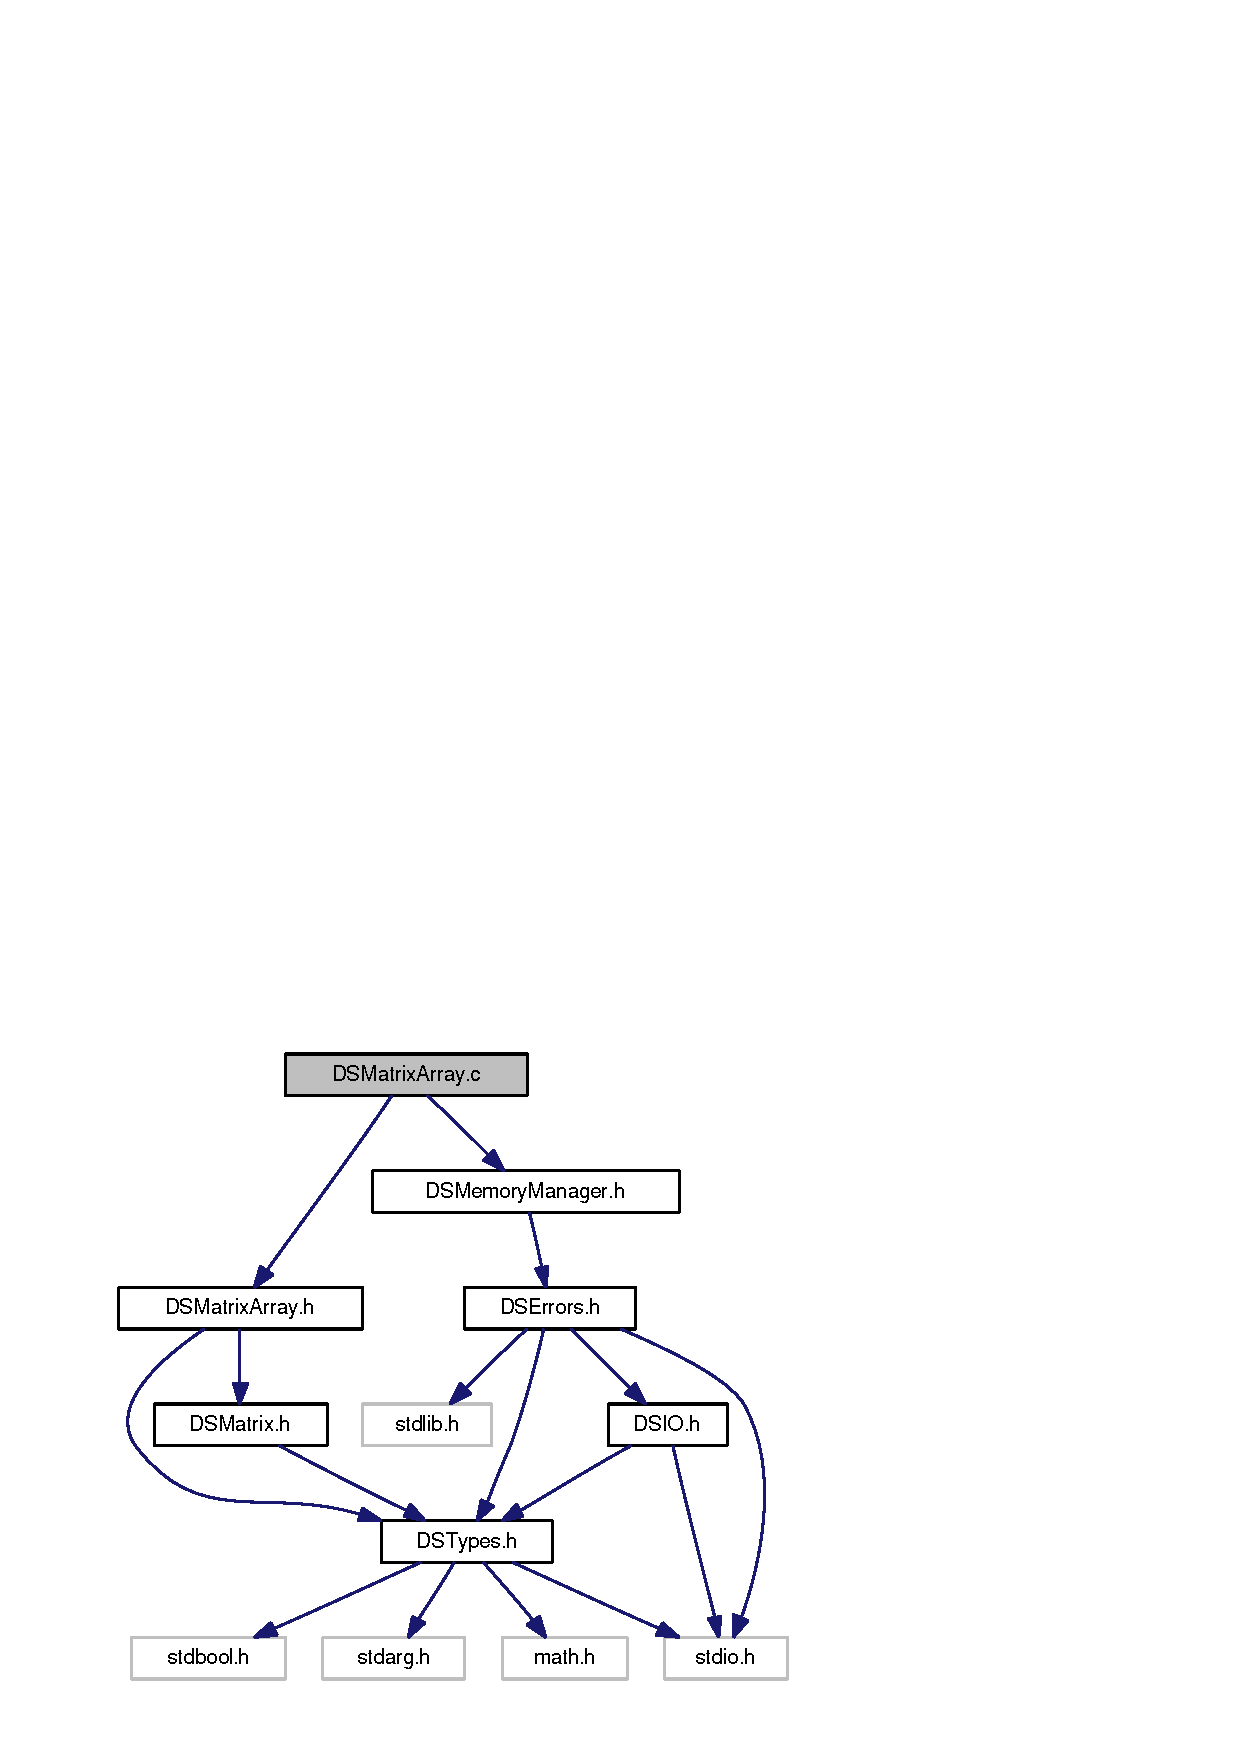
\includegraphics[width=193pt]{_d_s_matrix_array_8c__incl}
\end{center}
\end{figure}
\subsection*{Functions}
\begin{DoxyCompactItemize}
\item 
\hyperlink{struct_d_s_matrix_array}{DSMatrixArray} $\ast$ \hyperlink{_d_s_matrix_array_8c_ac28a8d64f99862378acc435e54c91c53}{DSMatrixArrayAlloc} (void)
\begin{DoxyCompactList}\small\item\em Memory allocation for a \hyperlink{struct_d_s_matrix_array}{DSMatrixArray}. \item\end{DoxyCompactList}\item 
\hyperlink{struct_d_s_matrix_array}{DSMatrixArray} $\ast$ \hyperlink{_d_s_matrix_array_8c_a694f4a21842a5e5bda0f4bdcb2e56626}{DSMatrixArrayCopy} (const \hyperlink{struct_d_s_matrix_array}{DSMatrixArray} $\ast$array)
\begin{DoxyCompactList}\small\item\em Copies a \hyperlink{struct_d_s_matrix_array}{DSMatrixArray}. \item\end{DoxyCompactList}\item 
void \hyperlink{_d_s_matrix_array_8c_a99f7d3e74613f43f22d8faa4bed25d1a}{DSMatrixArrayFree} (\hyperlink{struct_d_s_matrix_array}{DSMatrixArray} $\ast$array)
\begin{DoxyCompactList}\small\item\em Freeing memory for \hyperlink{struct_d_s_matrix_array}{DSMatrixArray}. \item\end{DoxyCompactList}\item 
\hyperlink{struct_d_s_matrix}{DSMatrix} $\ast$ \hyperlink{_d_s_matrix_array_8c_a4d9a430514e9384eea4a35ca826717c1}{DSMatrixArrayMatrix} (const \hyperlink{struct_d_s_matrix_array}{DSMatrixArray} $\ast$array, const DSUInteger index)
\begin{DoxyCompactList}\small\item\em Function to access a matrix in the \hyperlink{struct_d_s_matrix_array}{DSMatrixArray}. \item\end{DoxyCompactList}\item 
void \hyperlink{_d_s_matrix_array_8c_a91dd77e0cd7cff2173b6bfce9b9e7f4f}{DSMatrixArrayAddMatrix} (\hyperlink{struct_d_s_matrix_array}{DSMatrixArray} $\ast$array, const \hyperlink{struct_d_s_matrix}{DSMatrix} $\ast$matrixToAdd)
\begin{DoxyCompactList}\small\item\em Function to add a new matrix to the \hyperlink{struct_d_s_matrix_array}{DSMatrixArray}. \item\end{DoxyCompactList}\item 
\hypertarget{_d_s_matrix_array_8c_a78218c70cec38b886d663ad05c7031cf}{
double {\bfseries DSMatrixArrayDoubleWithIndices} (const \hyperlink{struct_d_s_matrix_array}{DSMatrixArray} $\ast$array, const DSUInteger i, const DSUInteger j, const DSUInteger k)}
\label{_d_s_matrix_array_8c_a78218c70cec38b886d663ad05c7031cf}

\item 
\hypertarget{_d_s_matrix_array_8c_ad4998c91be723d705130e33c3f554e14}{
void {\bfseries DSMatrixArrayPrint} (const \hyperlink{struct_d_s_matrix_array}{DSMatrixArray} $\ast$array)}
\label{_d_s_matrix_array_8c_ad4998c91be723d705130e33c3f554e14}

\end{DoxyCompactItemize}


\subsection{Detailed Description}
Implementation file with functions for dealing with matrix arrays. Copyright (C) 2011 Jason Lomnitz.\par
\par


This file is part of the Design Space Toolbox V2 (C Library).

The Design Space Toolbox V2 is free software: you can redistribute it and/or modify it under the terms of the GNU General Public License as published by the Free Software Foundation, either version 3 of the License, or (at your option) any later version.

The Design Space Toolbox V2 is distributed in the hope that it will be useful, but WITHOUT ANY WARRANTY; without even the implied warranty of MERCHANTABILITY or FITNESS FOR A PARTICULAR PURPOSE. See the GNU General Public License for more details.

You should have received a copy of the GNU General Public License along with the Design Space Toolbox. If not, see $<$\href{http://www.gnu.org/licenses/}{\tt http://www.gnu.org/licenses/}$>$.

\begin{DoxyAuthor}{Author}
Jason Lomnitz. 
\end{DoxyAuthor}
\begin{DoxyDate}{Date}
2011 
\end{DoxyDate}


\subsection{Function Documentation}
\hypertarget{_d_s_matrix_array_8c_a91dd77e0cd7cff2173b6bfce9b9e7f4f}{
\index{DSMatrixArray.c@{DSMatrixArray.c}!DSMatrixArrayAddMatrix@{DSMatrixArrayAddMatrix}}
\index{DSMatrixArrayAddMatrix@{DSMatrixArrayAddMatrix}!DSMatrixArray.c@{DSMatrixArray.c}}
\subsubsection[{DSMatrixArrayAddMatrix}]{\setlength{\rightskip}{0pt plus 5cm}void DSMatrixArrayAddMatrix ({\bf DSMatrixArray} $\ast$ {\em array}, \/  const {\bf DSMatrix} $\ast$ {\em matrixToAdd})}}
\label{_d_s_matrix_array_8c_a91dd77e0cd7cff2173b6bfce9b9e7f4f}


Function to add a new matrix to the \hyperlink{struct_d_s_matrix_array}{DSMatrixArray}. 

This function is the standard mechanism to add a \hyperlink{struct_d_s_matrix}{DSMatrix} to a \hyperlink{struct_d_s_matrix_array}{DSMatrixArray}. This function allocates the necessary space in the internal C array, and adds the \hyperlink{struct_d_s_matrix}{DSMatrix} to the end of the array. Once added to the matrix array, the memory is managed by the matrix array and is freed upon calling DSMatrixArrayFree.


\begin{DoxyParams}{Parameters}
\item[{\em array}]The \hyperlink{struct_d_s_matrix_array}{DSMatrixArray} that will have a new matrix added. \item[{\em matrixToAdd}]The \hyperlink{struct_d_s_matrix}{DSMatrix} to be added to the matrix array. \end{DoxyParams}
\hypertarget{_d_s_matrix_array_8c_ac28a8d64f99862378acc435e54c91c53}{
\index{DSMatrixArray.c@{DSMatrixArray.c}!DSMatrixArrayAlloc@{DSMatrixArrayAlloc}}
\index{DSMatrixArrayAlloc@{DSMatrixArrayAlloc}!DSMatrixArray.c@{DSMatrixArray.c}}
\subsubsection[{DSMatrixArrayAlloc}]{\setlength{\rightskip}{0pt plus 5cm}{\bf DSMatrixArray}$\ast$ DSMatrixArrayAlloc (void)}}
\label{_d_s_matrix_array_8c_ac28a8d64f99862378acc435e54c91c53}


Memory allocation for a \hyperlink{struct_d_s_matrix_array}{DSMatrixArray}. 

Creates a new \hyperlink{struct_d_s_matrix_array}{DSMatrixArray} with no matrices. As matrices are added, the matrix array grows, therefore the matrix array is initialized to 0, with a NULL internal pointer and number of matrices set to 0.

\begin{DoxyReturn}{Returns}
If the matrix array was created, a new pointer to a \hyperlink{struct_d_s_matrix}{DSMatrix} is returned. Otherwise, NULL is returned. 
\end{DoxyReturn}
\hypertarget{_d_s_matrix_array_8c_a694f4a21842a5e5bda0f4bdcb2e56626}{
\index{DSMatrixArray.c@{DSMatrixArray.c}!DSMatrixArrayCopy@{DSMatrixArrayCopy}}
\index{DSMatrixArrayCopy@{DSMatrixArrayCopy}!DSMatrixArray.c@{DSMatrixArray.c}}
\subsubsection[{DSMatrixArrayCopy}]{\setlength{\rightskip}{0pt plus 5cm}{\bf DSMatrixArray}$\ast$ DSMatrixArrayCopy (const {\bf DSMatrixArray} $\ast$ {\em array})}}
\label{_d_s_matrix_array_8c_a694f4a21842a5e5bda0f4bdcb2e56626}


Copies a \hyperlink{struct_d_s_matrix_array}{DSMatrixArray}. 

Creates a new \hyperlink{struct_d_s_matrix_array}{DSMatrixArray} with the exact same data and contents as some other matrix array. The matrices in the new \hyperlink{struct_d_s_matrix_array}{DSMatrixArray} are copies of the matrices in the original matrix array.


\begin{DoxyParams}{Parameters}
\item[{\em array}]The \hyperlink{struct_d_s_matrix_array}{DSMatrixArray} to be copied.\end{DoxyParams}
\begin{DoxyReturn}{Returns}
If the copy was succesful, a pointer to a copy of the \hyperlink{struct_d_s_matrix_array}{DSMatrixArray} is returned. Otherwise, NULL is returned.
\end{DoxyReturn}
\begin{DoxySeeAlso}{See also}
\hyperlink{_d_s_matrix__gsl_8c_a6d0f0f74bdd85829ba07dd33f51cfa11}{DSMatrixCopy} 
\end{DoxySeeAlso}
\hypertarget{_d_s_matrix_array_8c_a99f7d3e74613f43f22d8faa4bed25d1a}{
\index{DSMatrixArray.c@{DSMatrixArray.c}!DSMatrixArrayFree@{DSMatrixArrayFree}}
\index{DSMatrixArrayFree@{DSMatrixArrayFree}!DSMatrixArray.c@{DSMatrixArray.c}}
\subsubsection[{DSMatrixArrayFree}]{\setlength{\rightskip}{0pt plus 5cm}void DSMatrixArrayFree ({\bf DSMatrixArray} $\ast$ {\em array})}}
\label{_d_s_matrix_array_8c_a99f7d3e74613f43f22d8faa4bed25d1a}


Freeing memory for \hyperlink{struct_d_s_matrix_array}{DSMatrixArray}. 

Frees the memory associated with a \hyperlink{struct_d_s_matrix_array}{DSMatrixArray} data type. This function is a wrapper for the necessary steps needed to free the internal structure of the \hyperlink{struct_d_s_matrix_array}{DSMatrixArray}, this includes calling DSMatrixFree for each of the contained matrices, freeing the internal pointer to the array of matrices, and the \hyperlink{struct_d_s_matrix_array}{DSMatrixArray} data type itself.


\begin{DoxyParams}{Parameters}
\item[{\em array}]The \hyperlink{struct_d_s_matrix_array}{DSMatrixArray} to be freed. \end{DoxyParams}
\hypertarget{_d_s_matrix_array_8c_a4d9a430514e9384eea4a35ca826717c1}{
\index{DSMatrixArray.c@{DSMatrixArray.c}!DSMatrixArrayMatrix@{DSMatrixArrayMatrix}}
\index{DSMatrixArrayMatrix@{DSMatrixArrayMatrix}!DSMatrixArray.c@{DSMatrixArray.c}}
\subsubsection[{DSMatrixArrayMatrix}]{\setlength{\rightskip}{0pt plus 5cm}{\bf DSMatrix}$\ast$ DSMatrixArrayMatrix (const {\bf DSMatrixArray} $\ast$ {\em array}, \/  const DSUInteger {\em index})}}
\label{_d_s_matrix_array_8c_a4d9a430514e9384eea4a35ca826717c1}


Function to access a matrix in the \hyperlink{struct_d_s_matrix_array}{DSMatrixArray}. 

This accessor function returns the \hyperlink{struct_d_s_matrix}{DSMatrix} at the specified index of the \hyperlink{struct_d_s_matrix_array}{DSMatrixArray}. This function is the basic accessor function, and should always be used to access a matrix in a \hyperlink{struct_d_s_matrix_array}{DSMatrixArray}.


\begin{DoxyParams}{Parameters}
\item[{\em array}]The \hyperlink{struct_d_s_matrix_array}{DSMatrixArray} containing the matrix to be accessed. \item[{\em index}]The DSUInteger specifying the index in the C array of matrices contained in the \hyperlink{struct_d_s_matrix_array}{DSMatrixArray}.\end{DoxyParams}
\begin{DoxyReturn}{Returns}
If the \hyperlink{struct_d_s_matrix}{DSMatrix} at the specified index was found, the pointer to that matrix is returned. Otherwise, NULL is returned. 
\end{DoxyReturn}

\hypertarget{_d_s_matrix_array_8h}{
\section{DSMatrixArray.h File Reference}
\label{_d_s_matrix_array_8h}\index{DSMatrixArray.h@{DSMatrixArray.h}}
}


Header file with functions for dealing with matrix arrays.  


{\ttfamily \#include \char`\"{}DSTypes.h\char`\"{}}\par
{\ttfamily \#include \char`\"{}DSMatrix.h\char`\"{}}\par
Include dependency graph for DSMatrixArray.h:\nopagebreak
\begin{figure}[H]
\begin{center}
\leavevmode
\includegraphics[width=175pt]{_d_s_matrix_array_8h__incl}
\end{center}
\end{figure}
This graph shows which files directly or indirectly include this file:\nopagebreak
\begin{figure}[H]
\begin{center}
\leavevmode
\includegraphics[width=127pt]{_d_s_matrix_array_8h__dep__incl}
\end{center}
\end{figure}
\subsection*{Defines}
\begin{DoxyCompactItemize}
\item 
\hypertarget{_d_s_matrix_array_8h_ae5ed293af50a4fe892a5064c6f026fd5}{
\#define \hyperlink{_d_s_matrix_array_8h_ae5ed293af50a4fe892a5064c6f026fd5}{DSMatrixArrayNumberOfMatrices}(x)~((x)-\/$>$numberOfMatrices)}
\label{_d_s_matrix_array_8h_ae5ed293af50a4fe892a5064c6f026fd5}

\begin{DoxyCompactList}\small\item\em Accessor function to retrieve number of matrices in the Matrix array. \item\end{DoxyCompactList}\item 
\hypertarget{_d_s_matrix_array_8h_ad12db3a5ec12ae7eb52f988b529b4a80}{
\#define \hyperlink{_d_s_matrix_array_8h_ad12db3a5ec12ae7eb52f988b529b4a80}{DSMatrixArrayInternalPointer}(x)~((x)-\/$>$matrices)}
\label{_d_s_matrix_array_8h_ad12db3a5ec12ae7eb52f988b529b4a80}

\begin{DoxyCompactList}\small\item\em Accessor function to retrieve the pointer to the C matrix array. \item\end{DoxyCompactList}\end{DoxyCompactItemize}
\subsection*{Functions}
\begin{DoxyCompactItemize}
\item 
\hyperlink{struct_d_s_matrix_array}{DSMatrixArray} $\ast$ \hyperlink{_d_s_matrix_array_8h_ac28a8d64f99862378acc435e54c91c53}{DSMatrixArrayAlloc} (void)
\begin{DoxyCompactList}\small\item\em Memory allocation for a \hyperlink{struct_d_s_matrix_array}{DSMatrixArray}. \item\end{DoxyCompactList}\item 
\hyperlink{struct_d_s_matrix_array}{DSMatrixArray} $\ast$ \hyperlink{_d_s_matrix_array_8h_a694f4a21842a5e5bda0f4bdcb2e56626}{DSMatrixArrayCopy} (const \hyperlink{struct_d_s_matrix_array}{DSMatrixArray} $\ast$array)
\begin{DoxyCompactList}\small\item\em Copies a \hyperlink{struct_d_s_matrix_array}{DSMatrixArray}. \item\end{DoxyCompactList}\item 
void \hyperlink{_d_s_matrix_array_8h_a99f7d3e74613f43f22d8faa4bed25d1a}{DSMatrixArrayFree} (\hyperlink{struct_d_s_matrix_array}{DSMatrixArray} $\ast$array)
\begin{DoxyCompactList}\small\item\em Freeing memory for \hyperlink{struct_d_s_matrix_array}{DSMatrixArray}. \item\end{DoxyCompactList}\item 
\hyperlink{struct_d_s_matrix}{DSMatrix} $\ast$ \hyperlink{_d_s_matrix_array_8h_a4d9a430514e9384eea4a35ca826717c1}{DSMatrixArrayMatrix} (const \hyperlink{struct_d_s_matrix_array}{DSMatrixArray} $\ast$array, const DSUInteger index)
\begin{DoxyCompactList}\small\item\em Function to access a matrix in the \hyperlink{struct_d_s_matrix_array}{DSMatrixArray}. \item\end{DoxyCompactList}\item 
void \hyperlink{_d_s_matrix_array_8h_a91dd77e0cd7cff2173b6bfce9b9e7f4f}{DSMatrixArrayAddMatrix} (\hyperlink{struct_d_s_matrix_array}{DSMatrixArray} $\ast$array, const \hyperlink{struct_d_s_matrix}{DSMatrix} $\ast$matrixToAdd)
\begin{DoxyCompactList}\small\item\em Function to add a new matrix to the \hyperlink{struct_d_s_matrix_array}{DSMatrixArray}. \item\end{DoxyCompactList}\item 
\hypertarget{_d_s_matrix_array_8h_a78218c70cec38b886d663ad05c7031cf}{
double {\bfseries DSMatrixArrayDoubleWithIndices} (const \hyperlink{struct_d_s_matrix_array}{DSMatrixArray} $\ast$array, const DSUInteger i, const DSUInteger j, const DSUInteger k)}
\label{_d_s_matrix_array_8h_a78218c70cec38b886d663ad05c7031cf}

\item 
\hypertarget{_d_s_matrix_array_8h_ad4998c91be723d705130e33c3f554e14}{
void {\bfseries DSMatrixArrayPrint} (const \hyperlink{struct_d_s_matrix_array}{DSMatrixArray} $\ast$array)}
\label{_d_s_matrix_array_8h_ad4998c91be723d705130e33c3f554e14}

\end{DoxyCompactItemize}


\subsection{Detailed Description}
Header file with functions for dealing with matrix arrays. Copyright (C) 2011 Jason Lomnitz.\par
\par


This file is part of the Design Space Toolbox V2 (C Library).

The Design Space Toolbox V2 is free software: you can redistribute it and/or modify it under the terms of the GNU General Public License as published by the Free Software Foundation, either version 3 of the License, or (at your option) any later version.

The Design Space Toolbox V2 is distributed in the hope that it will be useful, but WITHOUT ANY WARRANTY; without even the implied warranty of MERCHANTABILITY or FITNESS FOR A PARTICULAR PURPOSE. See the GNU General Public License for more details.

You should have received a copy of the GNU General Public License along with the Design Space Toolbox. If not, see $<$\href{http://www.gnu.org/licenses/}{\tt http://www.gnu.org/licenses/}$>$.

\begin{DoxyAuthor}{Author}
Jason Lomnitz. 
\end{DoxyAuthor}
\begin{DoxyDate}{Date}
2011 
\end{DoxyDate}


\subsection{Function Documentation}
\hypertarget{_d_s_matrix_array_8h_a91dd77e0cd7cff2173b6bfce9b9e7f4f}{
\index{DSMatrixArray.h@{DSMatrixArray.h}!DSMatrixArrayAddMatrix@{DSMatrixArrayAddMatrix}}
\index{DSMatrixArrayAddMatrix@{DSMatrixArrayAddMatrix}!DSMatrixArray.h@{DSMatrixArray.h}}
\subsubsection[{DSMatrixArrayAddMatrix}]{\setlength{\rightskip}{0pt plus 5cm}void DSMatrixArrayAddMatrix ({\bf DSMatrixArray} $\ast$ {\em array}, \/  const {\bf DSMatrix} $\ast$ {\em matrixToAdd})}}
\label{_d_s_matrix_array_8h_a91dd77e0cd7cff2173b6bfce9b9e7f4f}


Function to add a new matrix to the \hyperlink{struct_d_s_matrix_array}{DSMatrixArray}. 

This function is the standard mechanism to add a \hyperlink{struct_d_s_matrix}{DSMatrix} to a \hyperlink{struct_d_s_matrix_array}{DSMatrixArray}. This function allocates the necessary space in the internal C array, and adds the \hyperlink{struct_d_s_matrix}{DSMatrix} to the end of the array. Once added to the matrix array, the memory is managed by the matrix array and is freed upon calling DSMatrixArrayFree.


\begin{DoxyParams}{Parameters}
\item[{\em array}]The \hyperlink{struct_d_s_matrix_array}{DSMatrixArray} that will have a new matrix added. \item[{\em matrixToAdd}]The \hyperlink{struct_d_s_matrix}{DSMatrix} to be added to the matrix array. \end{DoxyParams}
\hypertarget{_d_s_matrix_array_8h_ac28a8d64f99862378acc435e54c91c53}{
\index{DSMatrixArray.h@{DSMatrixArray.h}!DSMatrixArrayAlloc@{DSMatrixArrayAlloc}}
\index{DSMatrixArrayAlloc@{DSMatrixArrayAlloc}!DSMatrixArray.h@{DSMatrixArray.h}}
\subsubsection[{DSMatrixArrayAlloc}]{\setlength{\rightskip}{0pt plus 5cm}{\bf DSMatrixArray}$\ast$ DSMatrixArrayAlloc (void)}}
\label{_d_s_matrix_array_8h_ac28a8d64f99862378acc435e54c91c53}


Memory allocation for a \hyperlink{struct_d_s_matrix_array}{DSMatrixArray}. 

Creates a new \hyperlink{struct_d_s_matrix_array}{DSMatrixArray} with no matrices. As matrices are added, the matrix array grows, therefore the matrix array is initialized to 0, with a NULL internal pointer and number of matrices set to 0.

\begin{DoxyReturn}{Returns}
If the matrix array was created, a new pointer to a \hyperlink{struct_d_s_matrix}{DSMatrix} is returned. Otherwise, NULL is returned. 
\end{DoxyReturn}
\hypertarget{_d_s_matrix_array_8h_a694f4a21842a5e5bda0f4bdcb2e56626}{
\index{DSMatrixArray.h@{DSMatrixArray.h}!DSMatrixArrayCopy@{DSMatrixArrayCopy}}
\index{DSMatrixArrayCopy@{DSMatrixArrayCopy}!DSMatrixArray.h@{DSMatrixArray.h}}
\subsubsection[{DSMatrixArrayCopy}]{\setlength{\rightskip}{0pt plus 5cm}{\bf DSMatrixArray}$\ast$ DSMatrixArrayCopy (const {\bf DSMatrixArray} $\ast$ {\em array})}}
\label{_d_s_matrix_array_8h_a694f4a21842a5e5bda0f4bdcb2e56626}


Copies a \hyperlink{struct_d_s_matrix_array}{DSMatrixArray}. 

Creates a new \hyperlink{struct_d_s_matrix_array}{DSMatrixArray} with the exact same data and contents as some other matrix array. The matrices in the new \hyperlink{struct_d_s_matrix_array}{DSMatrixArray} are copies of the matrices in the original matrix array.


\begin{DoxyParams}{Parameters}
\item[{\em array}]The \hyperlink{struct_d_s_matrix_array}{DSMatrixArray} to be copied.\end{DoxyParams}
\begin{DoxyReturn}{Returns}
If the copy was succesful, a pointer to a copy of the \hyperlink{struct_d_s_matrix_array}{DSMatrixArray} is returned. Otherwise, NULL is returned.
\end{DoxyReturn}
\begin{DoxySeeAlso}{See also}
\hyperlink{_d_s_matrix__gsl_8c_a6d0f0f74bdd85829ba07dd33f51cfa11}{DSMatrixCopy} 
\end{DoxySeeAlso}
\hypertarget{_d_s_matrix_array_8h_a99f7d3e74613f43f22d8faa4bed25d1a}{
\index{DSMatrixArray.h@{DSMatrixArray.h}!DSMatrixArrayFree@{DSMatrixArrayFree}}
\index{DSMatrixArrayFree@{DSMatrixArrayFree}!DSMatrixArray.h@{DSMatrixArray.h}}
\subsubsection[{DSMatrixArrayFree}]{\setlength{\rightskip}{0pt plus 5cm}void DSMatrixArrayFree ({\bf DSMatrixArray} $\ast$ {\em array})}}
\label{_d_s_matrix_array_8h_a99f7d3e74613f43f22d8faa4bed25d1a}


Freeing memory for \hyperlink{struct_d_s_matrix_array}{DSMatrixArray}. 

Frees the memory associated with a \hyperlink{struct_d_s_matrix_array}{DSMatrixArray} data type. This function is a wrapper for the necessary steps needed to free the internal structure of the \hyperlink{struct_d_s_matrix_array}{DSMatrixArray}, this includes calling DSMatrixFree for each of the contained matrices, freeing the internal pointer to the array of matrices, and the \hyperlink{struct_d_s_matrix_array}{DSMatrixArray} data type itself.


\begin{DoxyParams}{Parameters}
\item[{\em array}]The \hyperlink{struct_d_s_matrix_array}{DSMatrixArray} to be freed. \end{DoxyParams}
\hypertarget{_d_s_matrix_array_8h_a4d9a430514e9384eea4a35ca826717c1}{
\index{DSMatrixArray.h@{DSMatrixArray.h}!DSMatrixArrayMatrix@{DSMatrixArrayMatrix}}
\index{DSMatrixArrayMatrix@{DSMatrixArrayMatrix}!DSMatrixArray.h@{DSMatrixArray.h}}
\subsubsection[{DSMatrixArrayMatrix}]{\setlength{\rightskip}{0pt plus 5cm}{\bf DSMatrix}$\ast$ DSMatrixArrayMatrix (const {\bf DSMatrixArray} $\ast$ {\em array}, \/  const DSUInteger {\em index})}}
\label{_d_s_matrix_array_8h_a4d9a430514e9384eea4a35ca826717c1}


Function to access a matrix in the \hyperlink{struct_d_s_matrix_array}{DSMatrixArray}. 

This accessor function returns the \hyperlink{struct_d_s_matrix}{DSMatrix} at the specified index of the \hyperlink{struct_d_s_matrix_array}{DSMatrixArray}. This function is the basic accessor function, and should always be used to access a matrix in a \hyperlink{struct_d_s_matrix_array}{DSMatrixArray}.


\begin{DoxyParams}{Parameters}
\item[{\em array}]The \hyperlink{struct_d_s_matrix_array}{DSMatrixArray} containing the matrix to be accessed. \item[{\em index}]The DSUInteger specifying the index in the C array of matrices contained in the \hyperlink{struct_d_s_matrix_array}{DSMatrixArray}.\end{DoxyParams}
\begin{DoxyReturn}{Returns}
If the \hyperlink{struct_d_s_matrix}{DSMatrix} at the specified index was found, the pointer to that matrix is returned. Otherwise, NULL is returned. 
\end{DoxyReturn}

\include{_d_s_memory_manager_8c}
\hypertarget{_d_s_memory_manager_8h}{
\section{DSMemoryManager.h File Reference}
\label{_d_s_memory_manager_8h}\index{DSMemoryManager.h@{DSMemoryManager.h}}
}


Header file with functions for secure memory allocation.  


{\ttfamily \#include \char`\"{}DSErrors.h\char`\"{}}\par
Include dependency graph for DSMemoryManager.h:\nopagebreak
\begin{figure}[H]
\begin{center}
\leavevmode
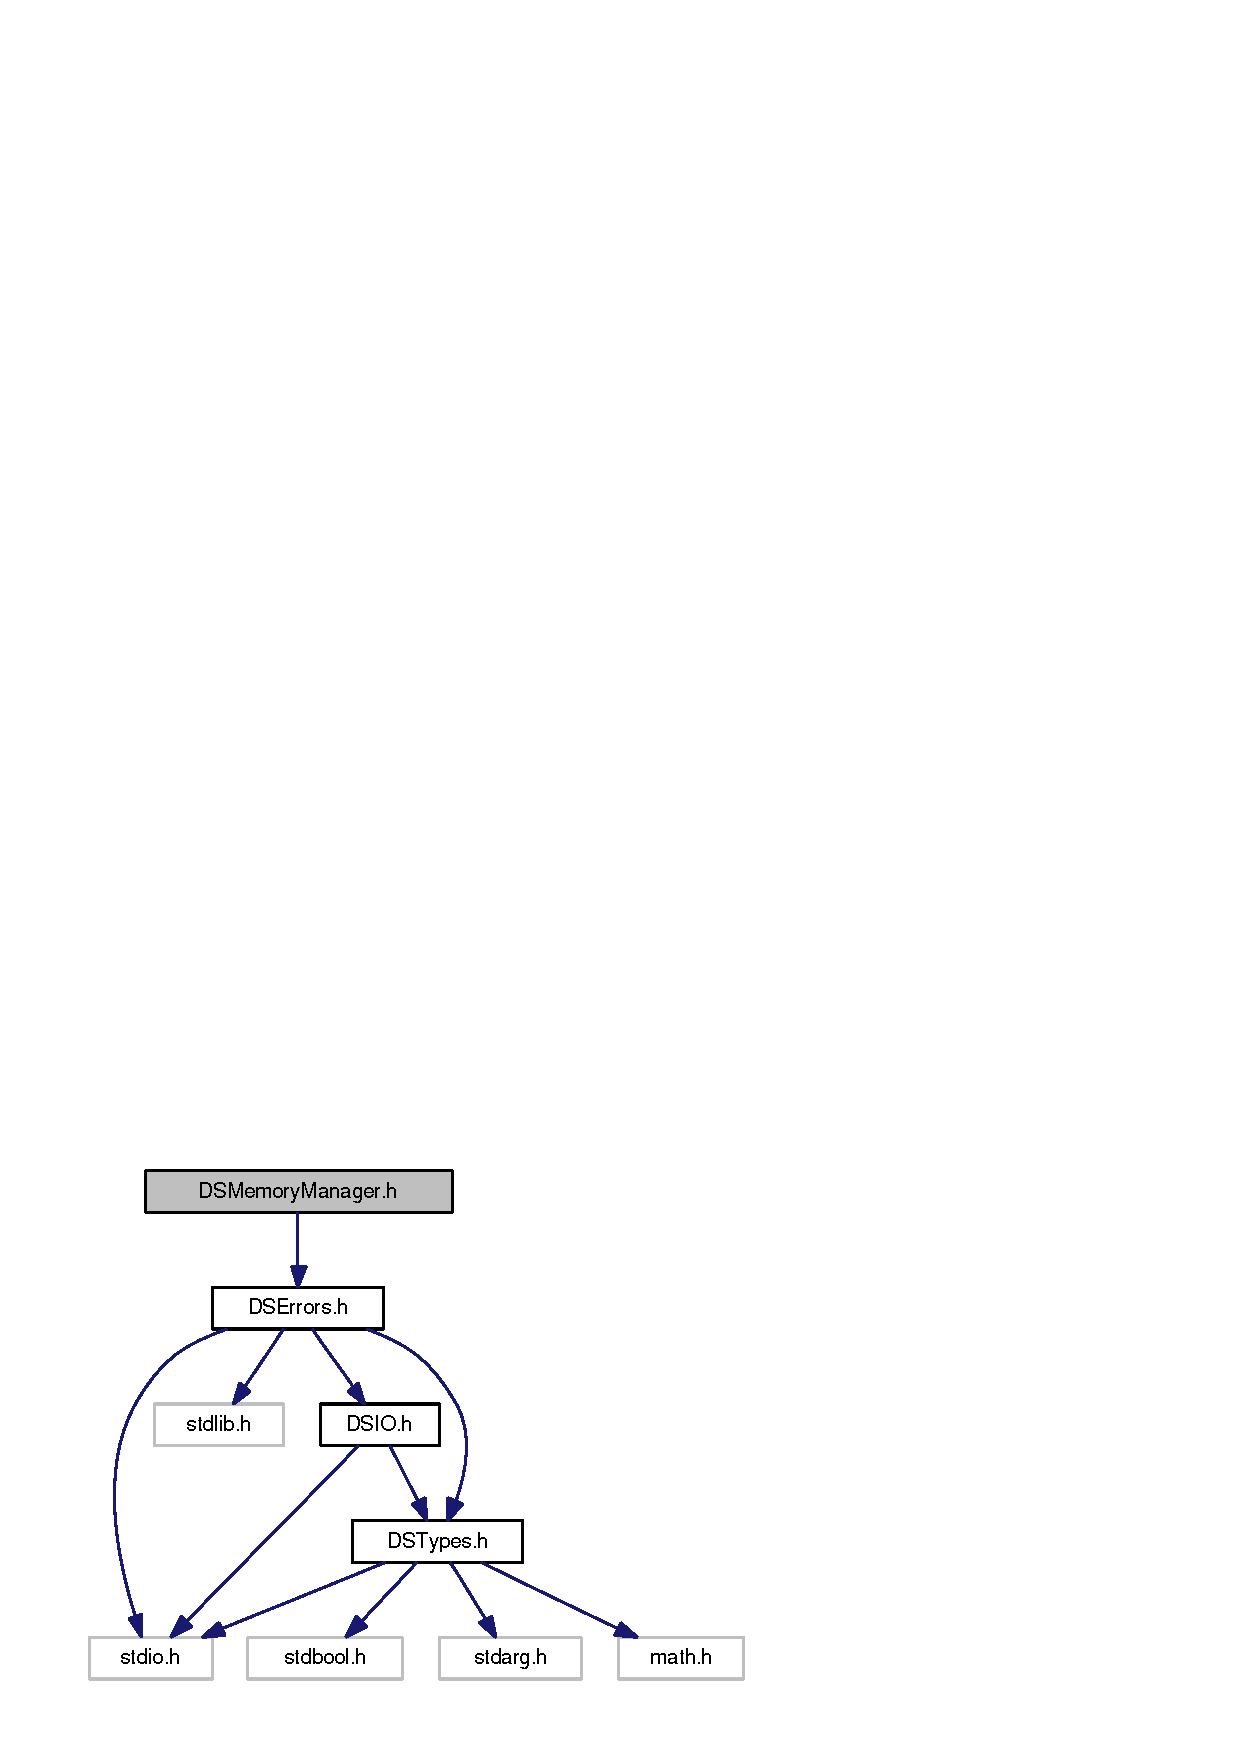
\includegraphics[width=179pt]{_d_s_memory_manager_8h__incl}
\end{center}
\end{figure}
This graph shows which files directly or indirectly include this file:\nopagebreak
\begin{figure}[H]
\begin{center}
\leavevmode
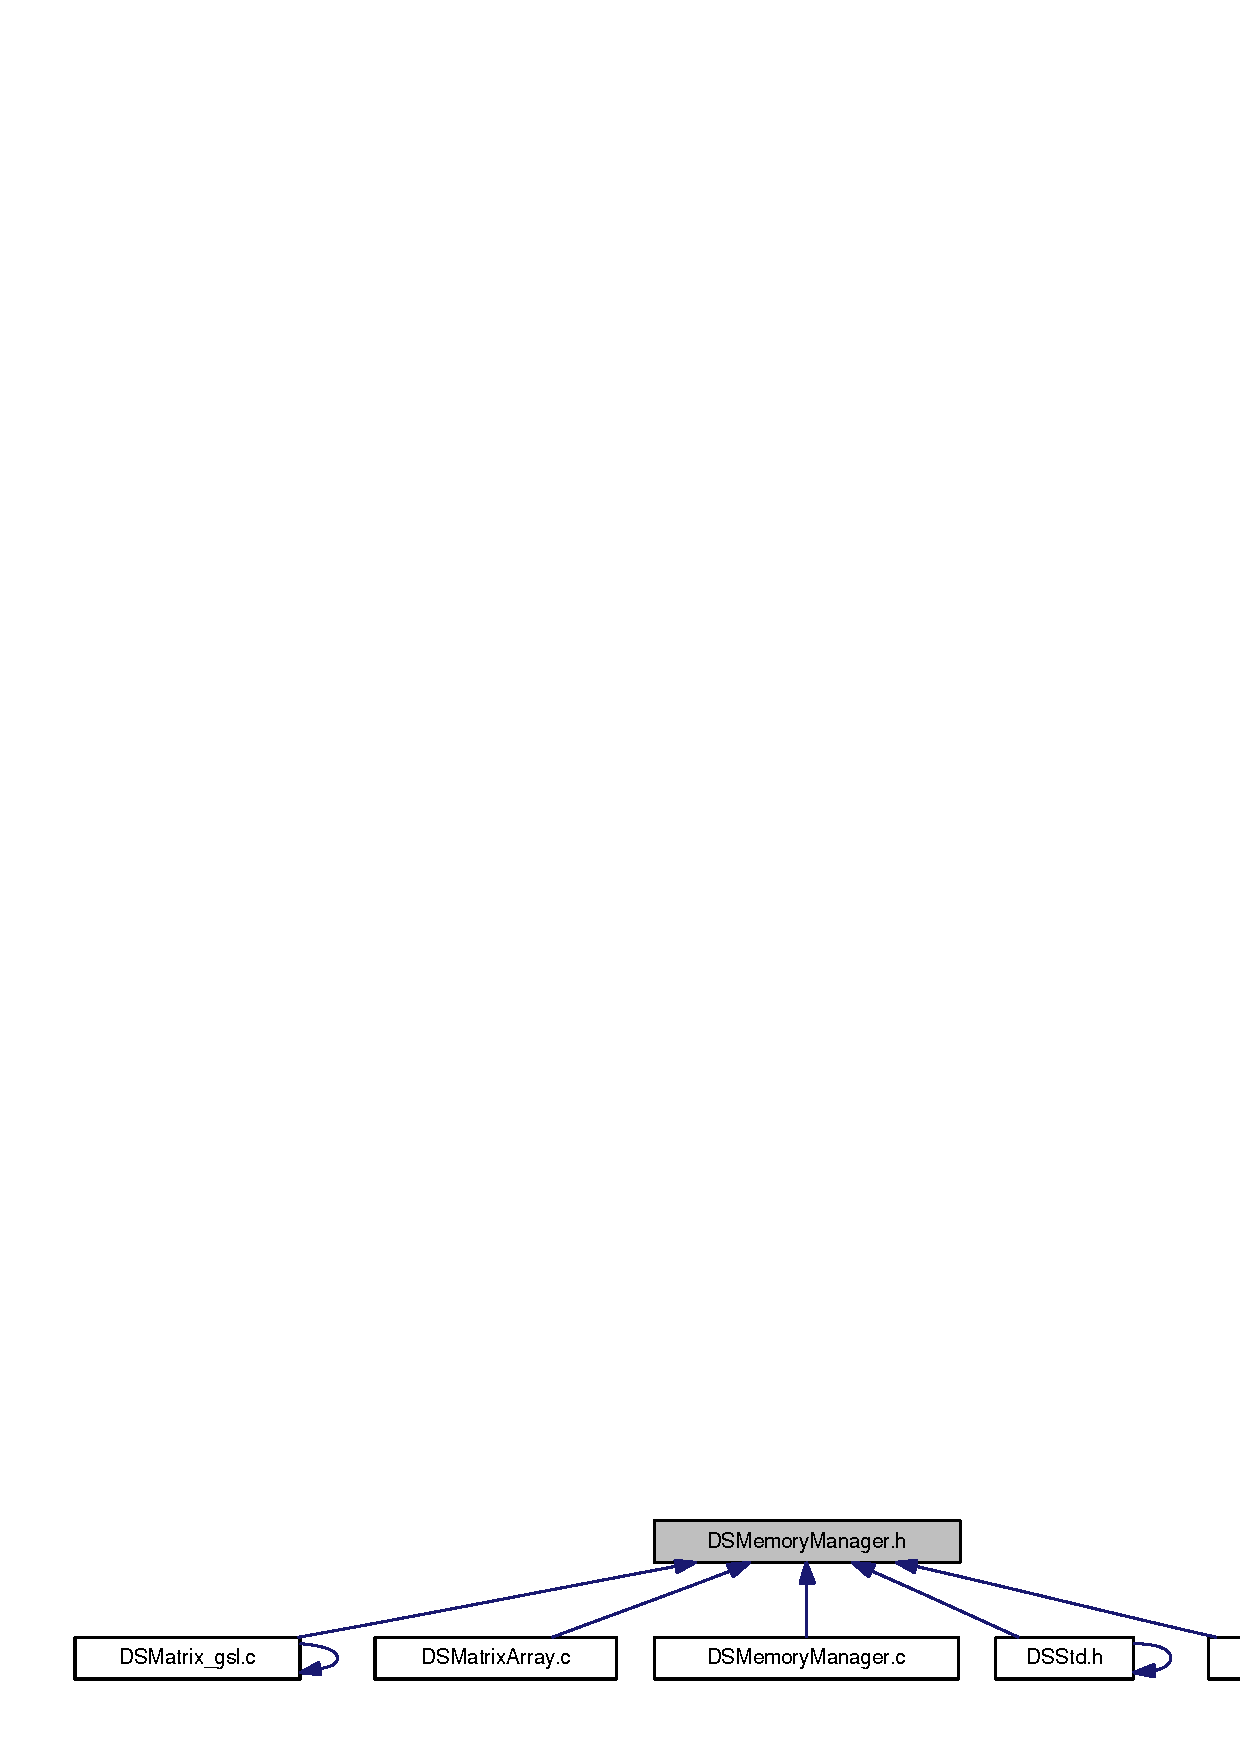
\includegraphics[width=337pt]{_d_s_memory_manager_8h__dep__incl}
\end{center}
\end{figure}
\subsection*{Functions}
\begin{DoxyCompactItemize}
\item 
void $\ast$ \hyperlink{_d_s_memory_manager_8h_a9563f15fd77be4f2dbf49880f6a69bd3}{DSSecureMalloc} (size\_\-t size)
\begin{DoxyCompactList}\small\item\em Function to securely allocate data using malloc. \item\end{DoxyCompactList}\item 
void $\ast$ \hyperlink{_d_s_memory_manager_8h_a67580b5d6039a40385a68d6570b8a440}{DSSecureCalloc} (size\_\-t count, size\_\-t size)
\begin{DoxyCompactList}\small\item\em Function to securely allocate data using calloc. \item\end{DoxyCompactList}\item 
void $\ast$ \hyperlink{_d_s_memory_manager_8h_abc98af878ea31098784da0b438364757}{DSSecureRealloc} (void $\ast$ptr, size\_\-t size)
\begin{DoxyCompactList}\small\item\em Function to securely allocate data using realloc. \item\end{DoxyCompactList}\item 
void \hyperlink{_d_s_memory_manager_8h_abf87115fd894707c20e7efb2108d1612}{DSSecureFree} (void $\ast$ptr)
\begin{DoxyCompactList}\small\item\em Function to securely free data. \item\end{DoxyCompactList}\end{DoxyCompactItemize}


\subsection{Detailed Description}
Header file with functions for secure memory allocation. This file specifies the design space standard for error handling. Contained here are the necessary macros and functions to succesfully report the errors throughout the design space library.

Copyright (C) 2011 Jason Lomnitz.\par
\par


This file is part of the Design Space Toolbox V2 (C Library).

The Design Space Toolbox V2 is free software: you can redistribute it and/or modify it under the terms of the GNU General Public License as published by the Free Software Foundation, either version 3 of the License, or (at your option) any later version.

The Design Space Toolbox V2 is distributed in the hope that it will be useful, but WITHOUT ANY WARRANTY; without even the implied warranty of MERCHANTABILITY or FITNESS FOR A PARTICULAR PURPOSE. See the GNU General Public License for more details.

You should have received a copy of the GNU General Public License along with the Design Space Toolbox. If not, see $<$\href{http://www.gnu.org/licenses/}{\tt http://www.gnu.org/licenses/}$>$.

\begin{DoxyAuthor}{Author}
Jason Lomnitz. 
\end{DoxyAuthor}
\begin{DoxyDate}{Date}
2011 
\end{DoxyDate}


\subsection{Function Documentation}
\hypertarget{_d_s_memory_manager_8h_a67580b5d6039a40385a68d6570b8a440}{
\index{DSMemoryManager.h@{DSMemoryManager.h}!DSSecureCalloc@{DSSecureCalloc}}
\index{DSSecureCalloc@{DSSecureCalloc}!DSMemoryManager.h@{DSMemoryManager.h}}
\subsubsection[{DSSecureCalloc}]{\setlength{\rightskip}{0pt plus 5cm}void$\ast$ DSSecureCalloc (size\_\-t {\em count}, \/  size\_\-t {\em size})}}
\label{_d_s_memory_manager_8h_a67580b5d6039a40385a68d6570b8a440}


Function to securely allocate data using calloc. 

This function is a secure calloc function which checks the allocated pointer. If the data pointer is null, indicative of errors allocating memory, the function issues a fatal error.


\begin{DoxyParams}{Parameters}
\item[{\em count}]A DSUInteger specifying the number of memory blocks being allocated. \item[{\em size}]The memory size of each block being allocated. \end{DoxyParams}
\begin{DoxyReturn}{Returns}
A pointer to the allocated data. 
\end{DoxyReturn}
\hypertarget{_d_s_memory_manager_8h_abf87115fd894707c20e7efb2108d1612}{
\index{DSMemoryManager.h@{DSMemoryManager.h}!DSSecureFree@{DSSecureFree}}
\index{DSSecureFree@{DSSecureFree}!DSMemoryManager.h@{DSMemoryManager.h}}
\subsubsection[{DSSecureFree}]{\setlength{\rightskip}{0pt plus 5cm}void DSSecureFree (void $\ast$ {\em ptr})}}
\label{_d_s_memory_manager_8h_abf87115fd894707c20e7efb2108d1612}


Function to securely free data. 

This function is a secure free function which checks the data pointer. If the data pointer is null, indicative of errors when freeing memory, the function issues a fatal error. This function calls malloc in case that pointer to be reallocated is NULL.


\begin{DoxyParams}{Parameters}
\item[{\em count}]A DSUInteger specifying the number of memory blocks being allocated. \item[{\em size}]The memory size of each block being allocated. \end{DoxyParams}
\begin{DoxyReturn}{Returns}
A pointer to the allocated data. 
\end{DoxyReturn}
\hypertarget{_d_s_memory_manager_8h_a9563f15fd77be4f2dbf49880f6a69bd3}{
\index{DSMemoryManager.h@{DSMemoryManager.h}!DSSecureMalloc@{DSSecureMalloc}}
\index{DSSecureMalloc@{DSSecureMalloc}!DSMemoryManager.h@{DSMemoryManager.h}}
\subsubsection[{DSSecureMalloc}]{\setlength{\rightskip}{0pt plus 5cm}void$\ast$ DSSecureMalloc (size\_\-t {\em size})}}
\label{_d_s_memory_manager_8h_a9563f15fd77be4f2dbf49880f6a69bd3}


Function to securely allocate data using malloc. 

This function is a secure malloc function which checks the allocated pointer. If the data pointer is null, indicative of errors allocating memory, the function issues a fatal error.


\begin{DoxyParams}{Parameters}
\item[{\em size}]A DSUInteger specifying the size of memory being allocated. \end{DoxyParams}
\begin{DoxyReturn}{Returns}
A pointer to the allocated data. 
\end{DoxyReturn}
\hypertarget{_d_s_memory_manager_8h_abc98af878ea31098784da0b438364757}{
\index{DSMemoryManager.h@{DSMemoryManager.h}!DSSecureRealloc@{DSSecureRealloc}}
\index{DSSecureRealloc@{DSSecureRealloc}!DSMemoryManager.h@{DSMemoryManager.h}}
\subsubsection[{DSSecureRealloc}]{\setlength{\rightskip}{0pt plus 5cm}void$\ast$ DSSecureRealloc (void $\ast$ {\em ptr}, \/  size\_\-t {\em size})}}
\label{_d_s_memory_manager_8h_abc98af878ea31098784da0b438364757}


Function to securely allocate data using realloc. 

This function is a secure realloc function which checks the allocated pointer. If the data pointer is null, indicative of errors allocating memory, the function issues a fatal error. This function calls malloc in case that pointer to be reallocated is NULL.


\begin{DoxyParams}{Parameters}
\item[{\em count}]A DSUInteger specifying the number of memory blocks being allocated. \item[{\em size}]The memory size of each block being allocated. \end{DoxyParams}
\begin{DoxyReturn}{Returns}
A pointer to the allocated data. 
\end{DoxyReturn}

\hypertarget{_d_s_std_8h}{
\section{DSStd.h File Reference}
\label{_d_s_std_8h}\index{DSStd.h@{DSStd.h}}
}


Header file for the design space toolbox.  


{\ttfamily \#include $<$stdio.h$>$}\par
{\ttfamily \#include $<$stdlib.h$>$}\par
{\ttfamily \#include \char`\"{}DSTypes.h\char`\"{}}\par
{\ttfamily \#include \char`\"{}DSIO.h\char`\"{}}\par
{\ttfamily \#include \char`\"{}DSErrors.h\char`\"{}}\par
{\ttfamily \#include \char`\"{}DSMemoryManager.h\char`\"{}}\par
{\ttfamily \#include \char`\"{}DSVariable.h\char`\"{}}\par
{\ttfamily \#include \char`\"{}DSMatrix.h\char`\"{}}\par
{\ttfamily \#include \char`\"{}DSMatrixArray.h\char`\"{}}\par
Include dependency graph for DSStd.h:\nopagebreak
\begin{figure}[H]
\begin{center}
\leavevmode
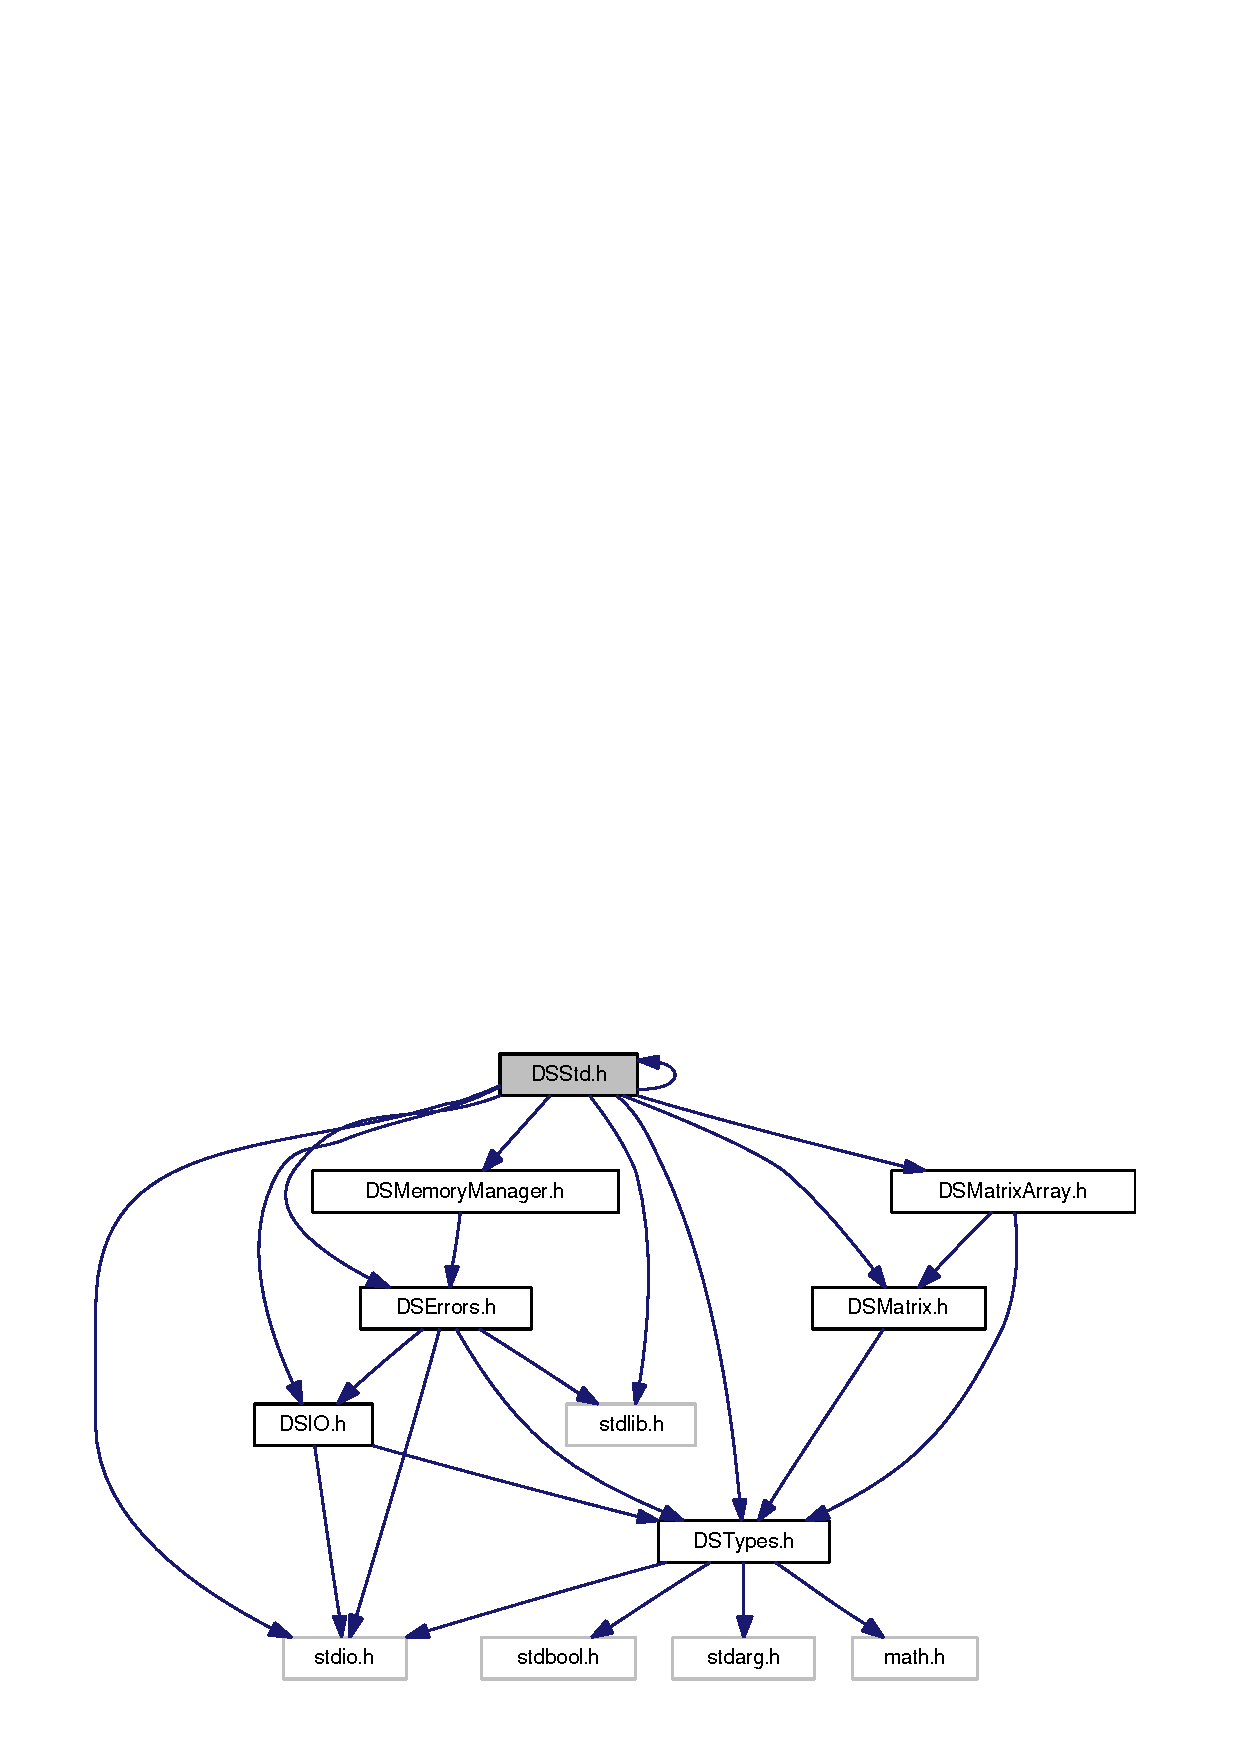
\includegraphics[width=272pt]{_d_s_std_8h__incl}
\end{center}
\end{figure}
This graph shows which files directly or indirectly include this file:\nopagebreak
\begin{figure}[H]
\begin{center}
\leavevmode
\includegraphics[width=60pt]{_d_s_std_8h__dep__incl}
\end{center}
\end{figure}


\subsection{Detailed Description}
Header file for the design space toolbox. Copyright (C) 2011 Jason Lomnitz.\par
\par


This file is part of the Design Space Toolbox V2 (C Library).

The Design Space Toolbox V2 is free software: you can redistribute it and/or modify it under the terms of the GNU General Public License as published by the Free Software Foundation, either version 3 of the License, or (at your option) any later version.

The Design Space Toolbox V2 is distributed in the hope that it will be useful, but WITHOUT ANY WARRANTY; without even the implied warranty of MERCHANTABILITY or FITNESS FOR A PARTICULAR PURPOSE. See the GNU General Public License for more details.

You should have received a copy of the GNU General Public License along with the Design Space Toolbox. If not, see $<$\href{http://www.gnu.org/licenses/}{\tt http://www.gnu.org/licenses/}$>$.

\begin{DoxyAuthor}{Author}
Jason Lomnitz. 
\end{DoxyAuthor}
\begin{DoxyDate}{Date}
2011
\end{DoxyDate}
\begin{Desc}
\item[\hyperlink{todo__todo000002}{Todo}]Add all previous functionality. 

Add vertex enumeration functionality.\end{Desc}

\hypertarget{_d_s_types_8h}{
\section{DSTypes.h File Reference}
\label{_d_s_types_8h}\index{DSTypes.h@{DSTypes.h}}
}


Header file with definitions for data types.  


{\ttfamily \#include $<$stdio.h$>$}\par
{\ttfamily \#include $<$stdbool.h$>$}\par
{\ttfamily \#include $<$stdarg.h$>$}\par
{\ttfamily \#include $<$math.h$>$}\par
Include dependency graph for DSTypes.h:\nopagebreak
\begin{figure}[H]
\begin{center}
\leavevmode
\includegraphics[width=175pt]{_d_s_types_8h__incl}
\end{center}
\end{figure}
This graph shows which files directly or indirectly include this file:\nopagebreak
\begin{figure}[H]
\begin{center}
\leavevmode
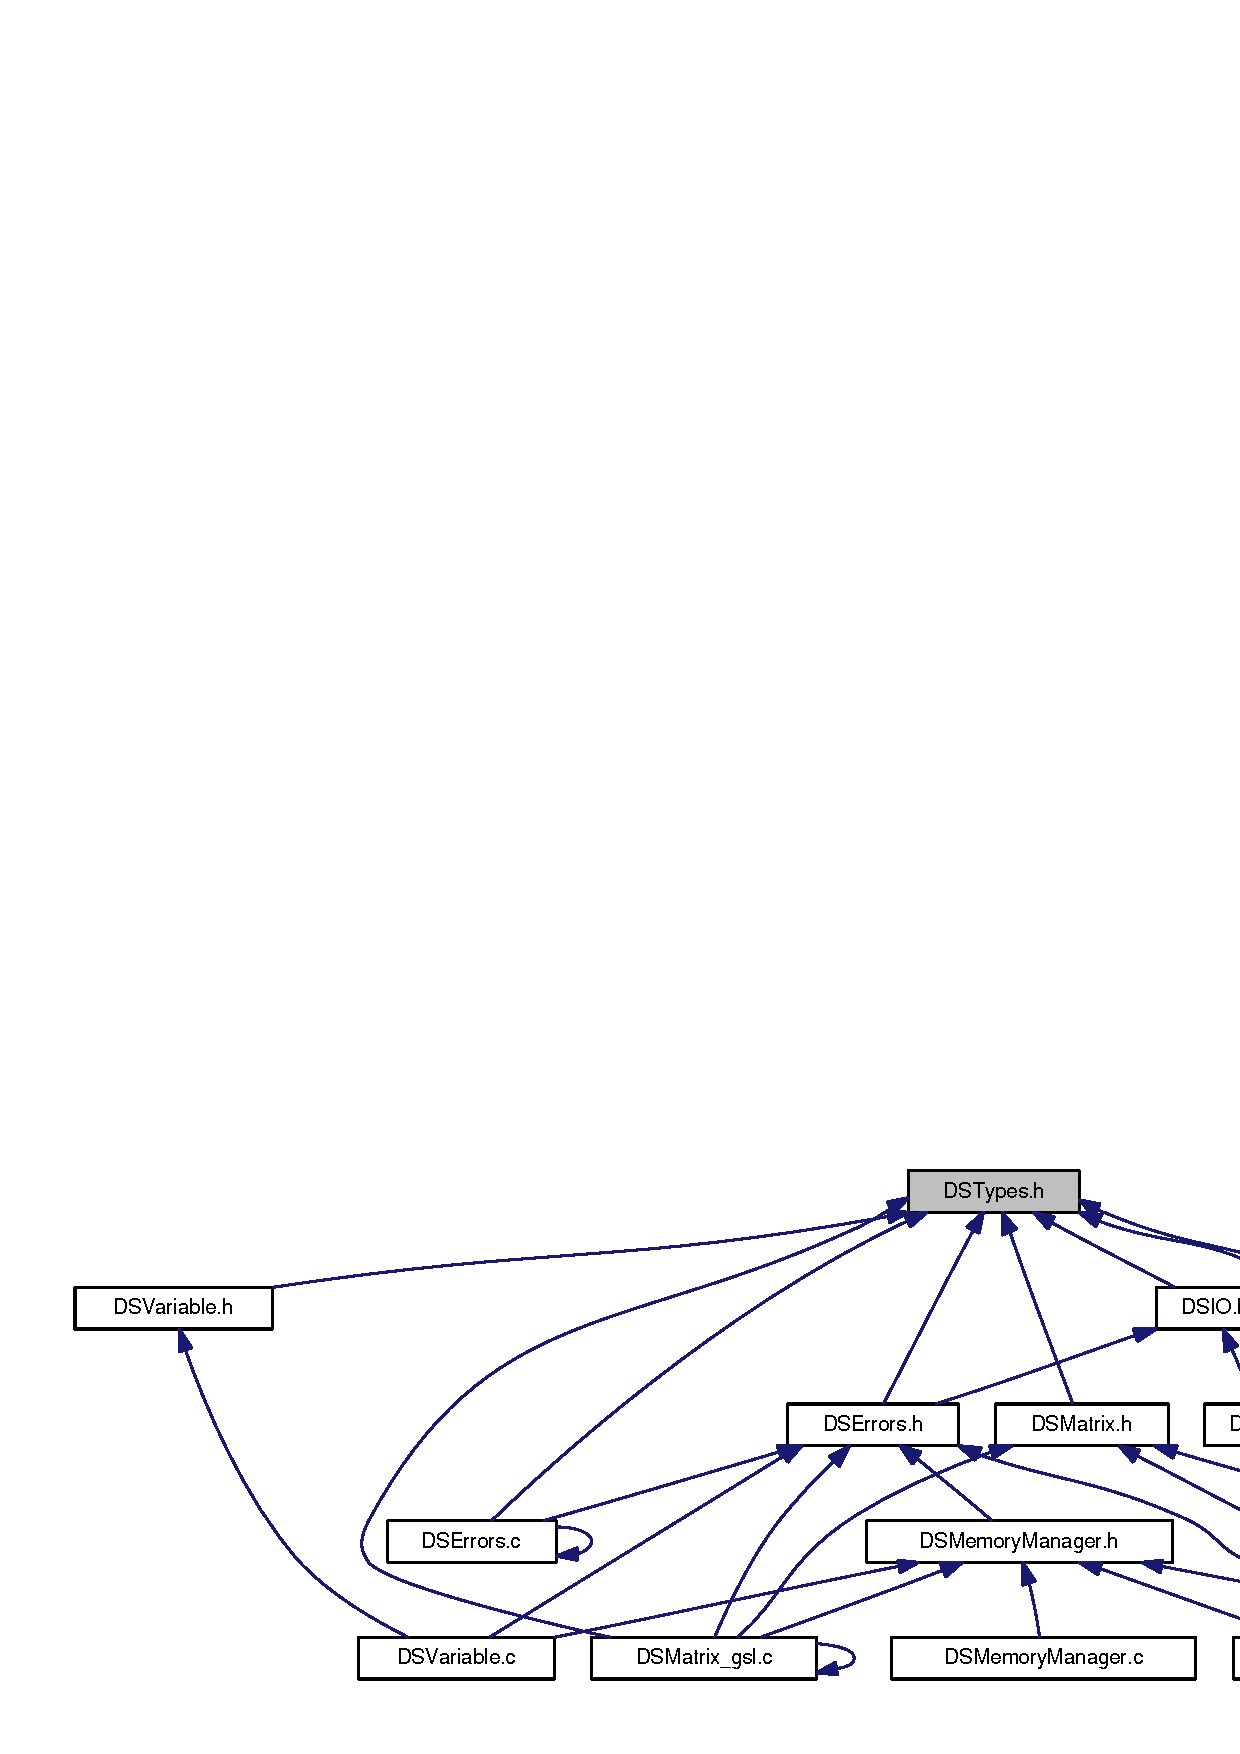
\includegraphics[width=420pt]{_d_s_types_8h__dep__incl}
\end{center}
\end{figure}
\subsection*{Data Structures}
\begin{DoxyCompactItemize}
\item 
struct \hyperlink{struct_d_s_variable}{DSVariable}
\begin{DoxyCompactList}\small\item\em Data type that is used to store errors. \item\end{DoxyCompactList}\item 
struct \hyperlink{struct__var_dictionary}{\_\-varDictionary}
\begin{DoxyCompactList}\small\item\em Internal dictionary structure. \item\end{DoxyCompactList}\item 
struct \hyperlink{struct_d_s_matrix}{DSMatrix}
\begin{DoxyCompactList}\small\item\em Data type representing a matrix. \item\end{DoxyCompactList}\item 
struct \hyperlink{struct_d_s_matrix_array}{DSMatrixArray}
\begin{DoxyCompactList}\small\item\em Data type representing an array of matrices. \item\end{DoxyCompactList}\item 
struct \hyperlink{struct_d_s_s_system}{DSSSystem}
\begin{DoxyCompactList}\small\item\em Data type representing an S-\/System. \item\end{DoxyCompactList}\end{DoxyCompactItemize}
\subsection*{Defines}
\begin{DoxyCompactItemize}
\item 
\hypertarget{_d_s_types_8h_aa0c1167bb311135eecf24a0e7c885b7f}{
\#define {\bfseries endif}}
\label{_d_s_types_8h_aa0c1167bb311135eecf24a0e7c885b7f}

\item 
\hypertarget{_d_s_types_8h_a4e1585cb1b8a465a6a9a702d97bb4ad8}{
\#define {\bfseries \_\-\_\-deprecated}}
\label{_d_s_types_8h_a4e1585cb1b8a465a6a9a702d97bb4ad8}

\item 
\hypertarget{_d_s_types_8h_a956e2723d559858d08644ac99146e910}{
\#define {\bfseries INFINITY}~HUGE\_\-VAL}
\label{_d_s_types_8h_a956e2723d559858d08644ac99146e910}

\end{DoxyCompactItemize}
\subsection*{Typedefs}
\begin{DoxyCompactItemize}
\item 
\hypertarget{_d_s_types_8h_acd52f160f8edb3f2c7c4ba8d9ddcd025}{
typedef int {\bfseries DSInteger}}
\label{_d_s_types_8h_acd52f160f8edb3f2c7c4ba8d9ddcd025}

\item 
\hypertarget{_d_s_types_8h_a176fc92c26d2116f67d6043e728adbb5}{
typedef unsigned int {\bfseries DSUInteger}}
\label{_d_s_types_8h_a176fc92c26d2116f67d6043e728adbb5}

\item 
typedef struct \hyperlink{struct__var_dictionary}{\_\-varDictionary} \hyperlink{_d_s_types_8h_a67b340fa4a564cc84d27b3647ef1ad75}{DSVariablePool}
\begin{DoxyCompactList}\small\item\em Internal dictionary structure. \item\end{DoxyCompactList}\end{DoxyCompactItemize}


\subsection{Detailed Description}
Header file with definitions for data types. This file specifies the design space standard data types. Contained here are strictly the data type definitions, and specific macros to access data in data structures. Functions applying to these data types are contained elsewhere, and the individual data structures should refer to these files.

Copyright (C) 2011 Jason Lomnitz.\par
\par


This file is part of the Design Space Toolbox V2 (C Library).

The Design Space Toolbox V2 is free software: you can redistribute it and/or modify it under the terms of the GNU General Public License as published by the Free Software Foundation, either version 3 of the License, or (at your option) any later version.

The Design Space Toolbox V2 is distributed in the hope that it will be useful, but WITHOUT ANY WARRANTY; without even the implied warranty of MERCHANTABILITY or FITNESS FOR A PARTICULAR PURPOSE. See the GNU General Public License for more details.

You should have received a copy of the GNU General Public License along with the Design Space Toolbox. If not, see $<$\href{http://www.gnu.org/licenses/}{\tt http://www.gnu.org/licenses/}$>$.

\begin{DoxyAuthor}{Author}
Jason Lomnitz. 
\end{DoxyAuthor}
\begin{DoxyDate}{Date}
2011 
\end{DoxyDate}


\subsection{Typedef Documentation}
\hypertarget{_d_s_types_8h_a67b340fa4a564cc84d27b3647ef1ad75}{
\index{DSTypes.h@{DSTypes.h}!DSVariablePool@{DSVariablePool}}
\index{DSVariablePool@{DSVariablePool}!DSTypes.h@{DSTypes.h}}
\subsubsection[{DSVariablePool}]{\setlength{\rightskip}{0pt plus 5cm}typedef struct {\bf \_\-varDictionary}  {\bf DSVariablePool}}}
\label{_d_s_types_8h_a67b340fa4a564cc84d27b3647ef1ad75}


Internal dictionary structure. 

Internal dictionary for fast variable querying. The structure of the dictionary uses an alternative path, where each character is checked in order at each position, if there is a match, the next position is consequently checked. The dictionary should never be manipulated manually, adding, retrieving and removing variables should be done through the accesory functions.

\begin{DoxySeeAlso}{See also}
\hyperlink{struct_d_s_variable}{DSVariable} 
\end{DoxySeeAlso}

\hypertarget{_d_s_variable_8c}{
\section{DSVariable.c File Reference}
\label{_d_s_variable_8c}\index{DSVariable.c@{DSVariable.c}}
}


Implementation file with functions for dealing with variables.  


{\ttfamily \#include $<$stdbool.h$>$}\par
{\ttfamily \#include $<$string.h$>$}\par
{\ttfamily \#include $<$math.h$>$}\par
{\ttfamily \#include \char`\"{}DSMemoryManager.h\char`\"{}}\par
{\ttfamily \#include \char`\"{}DSErrors.h\char`\"{}}\par
{\ttfamily \#include \char`\"{}DSVariable.h\char`\"{}}\par
Include dependency graph for DSVariable.c:\nopagebreak
\begin{figure}[H]
\begin{center}
\leavevmode
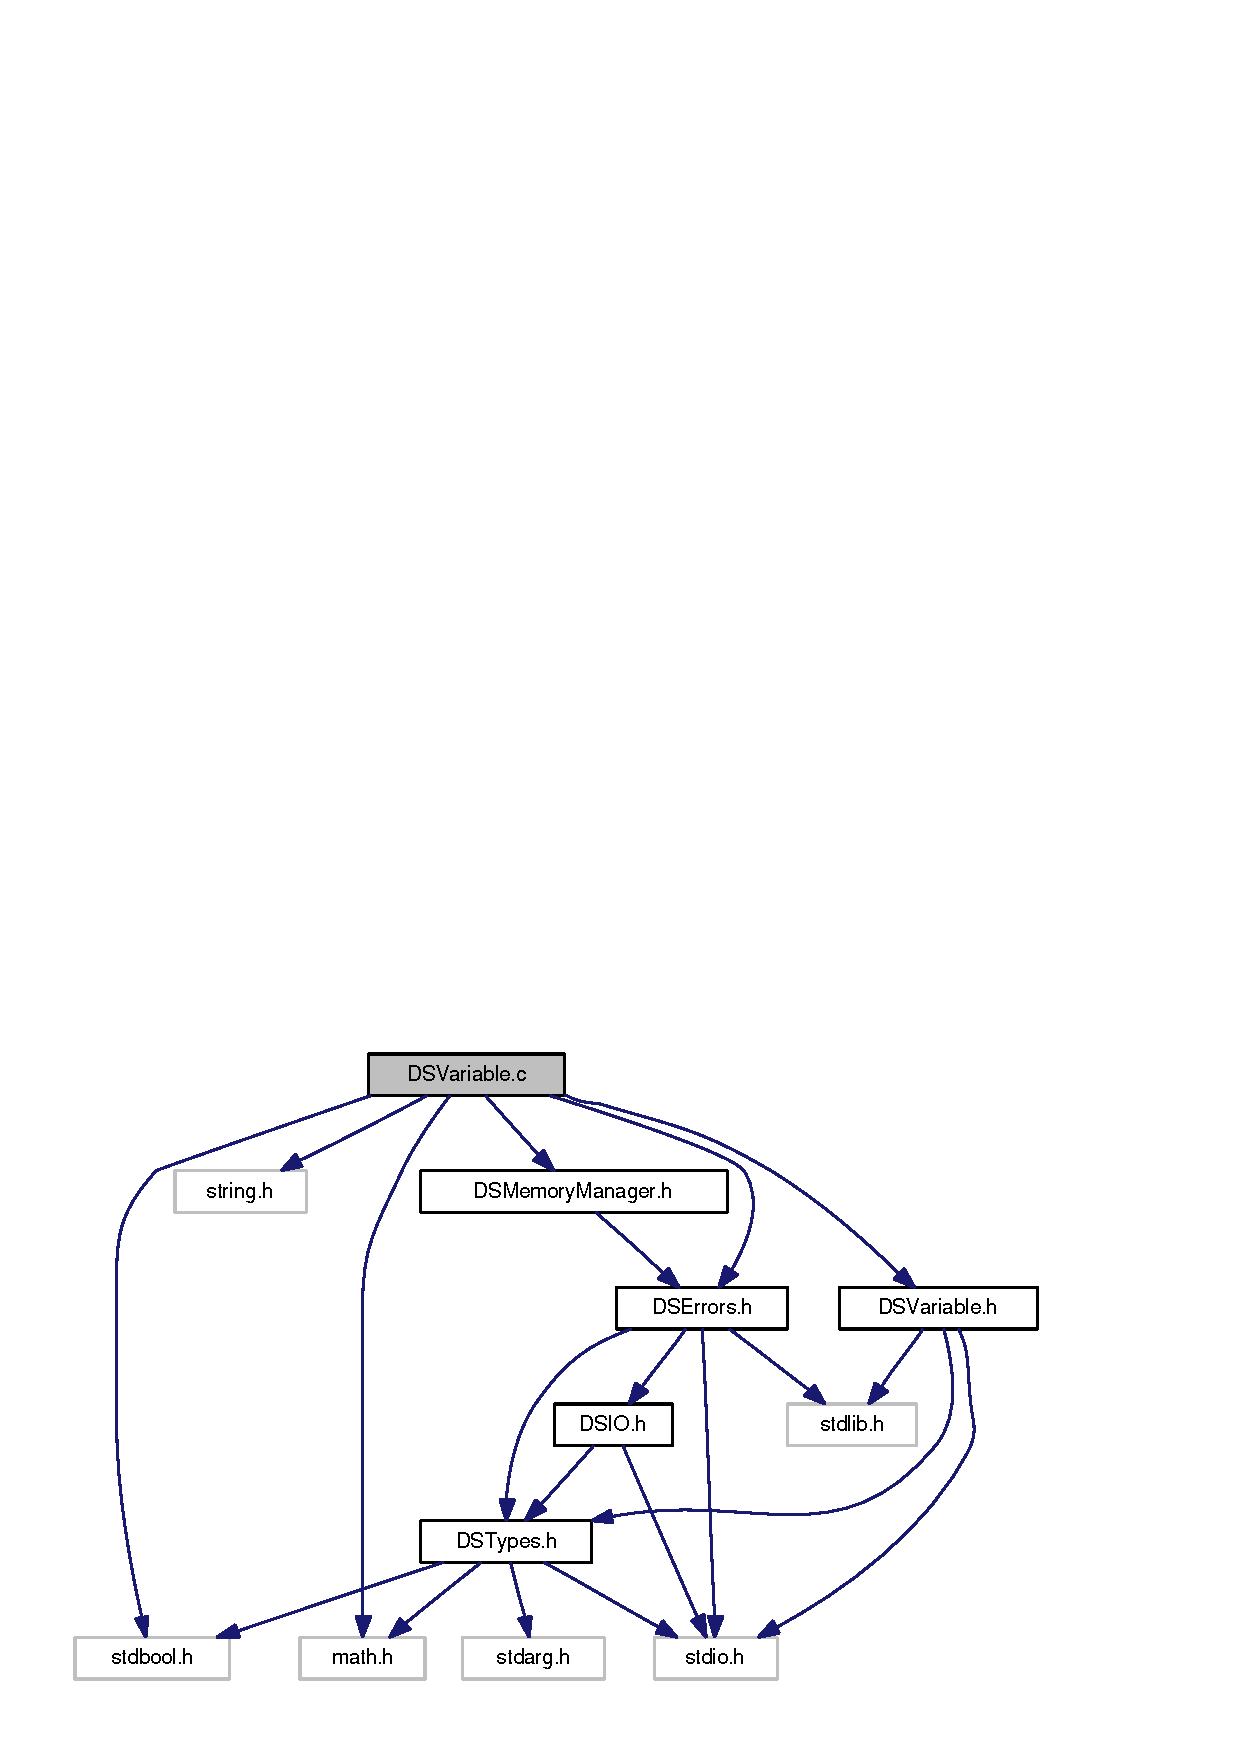
\includegraphics[width=258pt]{_d_s_variable_8c__incl}
\end{center}
\end{figure}
\subsection*{Functions}
\begin{DoxyCompactItemize}
\item 
\hyperlink{struct_d_s_variable}{DSVariable} $\ast$ \hyperlink{_d_s_variable_8c_a6f0ce189a8dc8ce46fad1d7a9b34d31f}{DSVariableAlloc} (const char $\ast$name)
\begin{DoxyCompactList}\small\item\em Creates a new \hyperlink{struct_d_s_variable}{DSVariable} with INFINITY as a default value. \item\end{DoxyCompactList}\item 
\hypertarget{_d_s_variable_8c_ac33e4c3da62459d2e356dd6456fca463}{
\hyperlink{struct_d_s_variable}{DSVariable} $\ast$ {\bfseries DSNewVariable} (const char $\ast$name)}
\label{_d_s_variable_8c_ac33e4c3da62459d2e356dd6456fca463}

\item 
void \hyperlink{_d_s_variable_8c_aac8fadf2969493124be37a1076a2b885}{DSVariableFree} (\hyperlink{struct_d_s_variable}{DSVariable} $\ast$var)
\begin{DoxyCompactList}\small\item\em Function frees allocated memory of a \hyperlink{struct_d_s_variable}{DSVariable}. \item\end{DoxyCompactList}\item 
\hyperlink{struct_d_s_variable}{DSVariable} $\ast$ \hyperlink{_d_s_variable_8c_a1a5da69573335a86dea1e4a8a6770ea3}{DSVariableRetain} (\hyperlink{struct_d_s_variable}{DSVariable} $\ast$aVariable)
\begin{DoxyCompactList}\small\item\em Function to increase variable retain count by one. \item\end{DoxyCompactList}\item 
void \hyperlink{_d_s_variable_8c_a4d83eec85c4d9340593a359fd1d5e506}{DSVariableRelease} (\hyperlink{struct_d_s_variable}{DSVariable} $\ast$aVariable)
\begin{DoxyCompactList}\small\item\em Function to decrease variable retain count by one. \item\end{DoxyCompactList}\item 
\hyperlink{struct__var_dictionary}{DSVariablePool} $\ast$ \hyperlink{_d_s_variable_8c_a4882cda43ad2d33bcafded6ed80e1fa6}{DSVariablePoolAddVariableWithName} (const char $\ast$name, \hyperlink{struct__var_dictionary}{DSVariablePool} $\ast$root)
\begin{DoxyCompactList}\small\item\em Adds a \hyperlink{struct_d_s_variable}{DSVariable} to the dictionary. \item\end{DoxyCompactList}\item 
\hyperlink{struct__var_dictionary}{DSVariablePool} $\ast$ \hyperlink{_d_s_variable_8c_aae1be18474aa9db03cb72912fd19234c}{DSVariablePoolAddVariable} (\hyperlink{struct_d_s_variable}{DSVariable} $\ast$newVar, \hyperlink{struct__var_dictionary}{DSVariablePool} $\ast$root)
\begin{DoxyCompactList}\small\item\em Adds a \hyperlink{struct_d_s_variable}{DSVariable} to the dictionary. \item\end{DoxyCompactList}\item 
\hyperlink{struct_d_s_variable}{DSVariable} $\ast$ \hyperlink{_d_s_variable_8c_ae8f75eb27aa14dda00f3251485d675ff}{DSVariablePoolVariableWithName} (const char $\ast$name, \hyperlink{struct__var_dictionary}{DSVariablePool} $\ast$root)
\begin{DoxyCompactList}\small\item\em Retrieves the variable in the dictionary with a matching name. \item\end{DoxyCompactList}\item 
\hypertarget{_d_s_variable_8c_a7c5942f23ebe838b353427df52522b2e}{
\hyperlink{struct_d_s_variable}{DSVariable} $\ast$ {\bfseries DSVariableWithName} (const char $\ast$name, \hyperlink{struct__var_dictionary}{DSVariablePool} $\ast$root)}
\label{_d_s_variable_8c_a7c5942f23ebe838b353427df52522b2e}

\item 
void \hyperlink{_d_s_variable_8c_aaed3132c306ffc004da9f391bbd1763c}{DSVariablePoolFree} (\hyperlink{struct__var_dictionary}{DSVariablePool} $\ast$root)
\begin{DoxyCompactList}\small\item\em Function to remove all nodes in the dictionary. \item\end{DoxyCompactList}\item 
void \hyperlink{_d_s_variable_8c_af16c50cbfa9139ef9e0dd828617816f2}{printVarDictionary} (\hyperlink{struct__var_dictionary}{DSVariablePool} $\ast$root, int indent)
\begin{DoxyCompactList}\small\item\em Prints the VarDictionary. \item\end{DoxyCompactList}\item 
void \hyperlink{_d_s_variable_8c_aa807b488d1b5c23e628a63e99ef8d0d9}{printMembers} (\hyperlink{struct__var_dictionary}{DSVariablePool} $\ast$root, char $\ast$buffer, int position)
\begin{DoxyCompactList}\small\item\em Function that prints the members in the dictionary. \item\end{DoxyCompactList}\end{DoxyCompactItemize}


\subsection{Detailed Description}
Implementation file with functions for dealing with variables. Copyright (C) 2011 Jason Lomnitz.\par
\par


This file is part of the Design Space Toolbox V2 (C Library).

The Design Space Toolbox V2 is free software: you can redistribute it and/or modify it under the terms of the GNU General Public License as published by the Free Software Foundation, either version 3 of the License, or (at your option) any later version.

The Design Space Toolbox V2 is distributed in the hope that it will be useful, but WITHOUT ANY WARRANTY; without even the implied warranty of MERCHANTABILITY or FITNESS FOR A PARTICULAR PURPOSE. See the GNU General Public License for more details.

You should have received a copy of the GNU General Public License along with the Design Space Toolbox. If not, see $<$\href{http://www.gnu.org/licenses/}{\tt http://www.gnu.org/licenses/}$>$.

\begin{DoxyAuthor}{Author}
Jason Lomnitz. 
\end{DoxyAuthor}
\begin{DoxyDate}{Date}
2011 
\end{DoxyDate}


\subsection{Function Documentation}
\hypertarget{_d_s_variable_8c_a6f0ce189a8dc8ce46fad1d7a9b34d31f}{
\index{DSVariable.c@{DSVariable.c}!DSVariableAlloc@{DSVariableAlloc}}
\index{DSVariableAlloc@{DSVariableAlloc}!DSVariable.c@{DSVariable.c}}
\subsubsection[{DSVariableAlloc}]{\setlength{\rightskip}{0pt plus 5cm}{\bf DSVariable}$\ast$ DSVariableAlloc (const char $\ast$ {\em name})}}
\label{_d_s_variable_8c_a6f0ce189a8dc8ce46fad1d7a9b34d31f}


Creates a new \hyperlink{struct_d_s_variable}{DSVariable} with INFINITY as a default value. 

This function may be used throughout, in order to create new variables consistently and portably. As variables are allocated individually, it is important to not that they should be released with the accesory method. 
\begin{DoxyParams}{Parameters}
\item[{\em name}]A string with which to identify the \hyperlink{struct_d_s_variable}{DSVariable}. \end{DoxyParams}
\begin{DoxyReturn}{Returns}
The pointer to the newly allocated \hyperlink{struct_d_s_variable}{DSVariable}. 
\end{DoxyReturn}
\begin{DoxySeeAlso}{See also}
\hyperlink{struct_d_s_variable}{DSVariable} 

\hyperlink{_d_s_variable_8h_aac8fadf2969493124be37a1076a2b885}{DSVariableFree} 
\end{DoxySeeAlso}
\hypertarget{_d_s_variable_8c_aac8fadf2969493124be37a1076a2b885}{
\index{DSVariable.c@{DSVariable.c}!DSVariableFree@{DSVariableFree}}
\index{DSVariableFree@{DSVariableFree}!DSVariable.c@{DSVariable.c}}
\subsubsection[{DSVariableFree}]{\setlength{\rightskip}{0pt plus 5cm}void DSVariableFree ({\bf DSVariable} $\ast$ {\em var})}}
\label{_d_s_variable_8c_aac8fadf2969493124be37a1076a2b885}


Function frees allocated memory of a \hyperlink{struct_d_s_variable}{DSVariable}. 

This function should be used for each newDSVariable that is called. The internal structure is subject to changes in consequent versions and therefore freeing memory of DSVariables should be strictly through this function. 
\begin{DoxyParams}{Parameters}
\item[{\em var}]The pointer to the variable to free. \end{DoxyParams}
\hypertarget{_d_s_variable_8c_aae1be18474aa9db03cb72912fd19234c}{
\index{DSVariable.c@{DSVariable.c}!DSVariablePoolAddVariable@{DSVariablePoolAddVariable}}
\index{DSVariablePoolAddVariable@{DSVariablePoolAddVariable}!DSVariable.c@{DSVariable.c}}
\subsubsection[{DSVariablePoolAddVariable}]{\setlength{\rightskip}{0pt plus 5cm}{\bf DSVariablePool}$\ast$ DSVariablePoolAddVariable ({\bf DSVariable} $\ast$ {\em newVar}, \/  {\bf DSVariablePool} $\ast$ {\em root})}}
\label{_d_s_variable_8c_aae1be18474aa9db03cb72912fd19234c}


Adds a \hyperlink{struct_d_s_variable}{DSVariable} to the dictionary. 

This is the function to add DSVariables to the dictionary. Since the dictionary works alphabetically, the root of the dictionary changes and is defined by this function, and the root, be it the new one or the old one, is returned. This function is used in creating a new dictionary. 
\begin{DoxyParams}{Parameters}
\item[{\em newVar}]The pointer to the variable which is to be added to the dictionary. \item[{\em root}]The root of the dictionary. THE ROOT MAY BE REASSIGNED. If null, creates a new dictionary. \end{DoxyParams}
\begin{DoxyReturn}{Returns}
The root of the dictionary, which is likely to change. 
\end{DoxyReturn}
\begin{DoxySeeAlso}{See also}
\hyperlink{struct__var_dictionary}{\_\-varDictionary} 

DSVariableWithName 

\_\-addNewBranch 
\end{DoxySeeAlso}
\hypertarget{_d_s_variable_8c_a4882cda43ad2d33bcafded6ed80e1fa6}{
\index{DSVariable.c@{DSVariable.c}!DSVariablePoolAddVariableWithName@{DSVariablePoolAddVariableWithName}}
\index{DSVariablePoolAddVariableWithName@{DSVariablePoolAddVariableWithName}!DSVariable.c@{DSVariable.c}}
\subsubsection[{DSVariablePoolAddVariableWithName}]{\setlength{\rightskip}{0pt plus 5cm}{\bf DSVariablePool}$\ast$ DSVariablePoolAddVariableWithName (const char $\ast$ {\em name}, \/  {\bf DSVariablePool} $\ast$ {\em root})}}
\label{_d_s_variable_8c_a4882cda43ad2d33bcafded6ed80e1fa6}


Adds a \hyperlink{struct_d_s_variable}{DSVariable} to the dictionary. 

This is the function to add DSVariables to the dictionary. Since the dictionary works alphabetically, the root of the dictionary changes and is defined by this function, and the root, be it the new one or the old one, is returned. This function is used in creating a new dictionary. 
\begin{DoxyParams}{Parameters}
\item[{\em newVar}]The pointer to the variable which is to be added to the dictionary. \item[{\em root}]The root of the dictionary. THE ROOT MAY BE REASSIGNED. If null, creates a new dictionary. \end{DoxyParams}
\begin{DoxyReturn}{Returns}
The root of the dictionary, which is likely to change. 
\end{DoxyReturn}
\begin{DoxySeeAlso}{See also}
\hyperlink{struct__var_dictionary}{\_\-varDictionary} 

DSVariableWithName 

\_\-addNewBranch 
\end{DoxySeeAlso}
\hypertarget{_d_s_variable_8c_aaed3132c306ffc004da9f391bbd1763c}{
\index{DSVariable.c@{DSVariable.c}!DSVariablePoolFree@{DSVariablePoolFree}}
\index{DSVariablePoolFree@{DSVariablePoolFree}!DSVariable.c@{DSVariable.c}}
\subsubsection[{DSVariablePoolFree}]{\setlength{\rightskip}{0pt plus 5cm}void DSVariablePoolFree ({\bf DSVariablePool} $\ast$ {\em root})}}
\label{_d_s_variable_8c_aaed3132c306ffc004da9f391bbd1763c}


Function to remove all nodes in the dictionary. 

The function is RECURSIVE and frees all the nodes past the root which is passed. In theory, it could be used to clear a portion of the dictionary, yet doing so would require direct manipulation of the dictionary which is strongly discouraged. The variables themselves are NOT freed, since the dictionary does not allocate them. 
\begin{DoxyParams}{Parameters}
\item[{\em root}]The root of the dictionary which is to be cleared. \end{DoxyParams}
\begin{DoxySeeAlso}{See also}
\hyperlink{_d_s_types_8h_a67b340fa4a564cc84d27b3647ef1ad75}{DSVariablePool} 

DSVariableWithName 

\hyperlink{_d_s_variable_8h_aae1be18474aa9db03cb72912fd19234c}{DSVariablePoolAddVariable} 
\end{DoxySeeAlso}
\hypertarget{_d_s_variable_8c_ae8f75eb27aa14dda00f3251485d675ff}{
\index{DSVariable.c@{DSVariable.c}!DSVariablePoolVariableWithName@{DSVariablePoolVariableWithName}}
\index{DSVariablePoolVariableWithName@{DSVariablePoolVariableWithName}!DSVariable.c@{DSVariable.c}}
\subsubsection[{DSVariablePoolVariableWithName}]{\setlength{\rightskip}{0pt plus 5cm}{\bf DSVariable}$\ast$ DSVariablePoolVariableWithName (const char $\ast$ {\em name}, \/  {\bf DSVariablePool} $\ast$ {\em root})}}
\label{_d_s_variable_8c_ae8f75eb27aa14dda00f3251485d675ff}


Retrieves the variable in the dictionary with a matching name. 

This is the function for retriving a \hyperlink{struct_d_s_variable}{DSVariable} from a dictionary. 
\begin{DoxyParams}{Parameters}
\item[{\em name}]A string containing a NULL terminated string containing the name of the desired \hyperlink{struct_d_s_variable}{DSVariable}. \item[{\em root}]The root of the dictionary, determined during the adding of variables. \end{DoxyParams}
\begin{DoxyReturn}{Returns}
A pointer to the variable. If there is no matching variable, NULL is returned. 
\end{DoxyReturn}
\begin{DoxySeeAlso}{See also}
\_\-checkNameAtPos 

\hyperlink{_d_s_types_8h_a67b340fa4a564cc84d27b3647ef1ad75}{DSVariablePool} 

\hyperlink{_d_s_variable_8h_aae1be18474aa9db03cb72912fd19234c}{DSVariablePoolAddVariable} 
\end{DoxySeeAlso}
\hypertarget{_d_s_variable_8c_a4d83eec85c4d9340593a359fd1d5e506}{
\index{DSVariable.c@{DSVariable.c}!DSVariableRelease@{DSVariableRelease}}
\index{DSVariableRelease@{DSVariableRelease}!DSVariable.c@{DSVariable.c}}
\subsubsection[{DSVariableRelease}]{\setlength{\rightskip}{0pt plus 5cm}void DSVariableRelease ({\bf DSVariable} $\ast$ {\em aVariable})}}
\label{_d_s_variable_8c_a4d83eec85c4d9340593a359fd1d5e506}


Function to decrease variable retain count by one. 

Fast processing tree is made to decrease its retain count by one, when the retain count hits zero, the function \hyperlink{_d_s_variable_8c_aac8fadf2969493124be37a1076a2b885}{DSVariableFree()} is invoked, freeing the memory space. Fast processing tree does not have an equivalent to autorelease, forcing the developer to use greater care when directly managing memory.


\begin{DoxyParams}{Parameters}
\item[{\em aVariable}]The variable which will have its retain count reduced.\end{DoxyParams}
\begin{DoxySeeAlso}{See also}
\hyperlink{_d_s_variable_8h_a1a5da69573335a86dea1e4a8a6770ea3}{DSVariableRetain} 

\hyperlink{_d_s_variable_8h_aac8fadf2969493124be37a1076a2b885}{DSVariableFree} 
\end{DoxySeeAlso}
\hypertarget{_d_s_variable_8c_a1a5da69573335a86dea1e4a8a6770ea3}{
\index{DSVariable.c@{DSVariable.c}!DSVariableRetain@{DSVariableRetain}}
\index{DSVariableRetain@{DSVariableRetain}!DSVariable.c@{DSVariable.c}}
\subsubsection[{DSVariableRetain}]{\setlength{\rightskip}{0pt plus 5cm}{\bf DSVariable}$\ast$ DSVariableRetain ({\bf DSVariable} $\ast$ {\em aVariable})}}
\label{_d_s_variable_8c_a1a5da69573335a86dea1e4a8a6770ea3}


Function to increase variable retain count by one. 

Variables utilize a similar memory management system used in Objective-\/C NSObject subclasses, where objects a retained/released.


\begin{DoxyParams}{Parameters}
\item[{\em aVariable}]The variable which will have its retain count increased.\end{DoxyParams}
\begin{DoxyReturn}{Returns}
The same variable which received the retain count increase is returned, for convinience.
\end{DoxyReturn}
\begin{DoxySeeAlso}{See also}
\hyperlink{_d_s_variable_8h_a4d83eec85c4d9340593a359fd1d5e506}{DSVariableRelease} 
\end{DoxySeeAlso}
\hypertarget{_d_s_variable_8c_aa807b488d1b5c23e628a63e99ef8d0d9}{
\index{DSVariable.c@{DSVariable.c}!printMembers@{printMembers}}
\index{printMembers@{printMembers}!DSVariable.c@{DSVariable.c}}
\subsubsection[{printMembers}]{\setlength{\rightskip}{0pt plus 5cm}void printMembers ({\bf DSVariablePool} $\ast$ {\em root}, \/  char $\ast$ {\em buffer}, \/  int {\em position})}}
\label{_d_s_variable_8c_aa807b488d1b5c23e628a63e99ef8d0d9}


Function that prints the members in the dictionary. 

This function recursively checks the dictionary for all names, and prints them out. It requires of a buffer string which is used to store the current characters, since it is a recursive function. 
\begin{DoxyParams}{Parameters}
\item[{\em root}]The root of the dictionary, and the current node for consequent calls. \item[{\em buffer}]The string in which to store the characters, function does not check size of buffer. \item[{\em position}]Should be 0 when called, increases as it searches the dictionary. \end{DoxyParams}
\begin{DoxySeeAlso}{See also}
\hyperlink{struct__var_dictionary}{\_\-varDictionary} 

\hyperlink{_d_s_variable_8h_aae1be18474aa9db03cb72912fd19234c}{DSVariablePoolAddVariable} 
\end{DoxySeeAlso}
\begin{Desc}
\item[\hyperlink{todo__todo000003}{Todo}]Create a wrapper function which creates the buffer, and initiates the position at 0. \end{Desc}
\hypertarget{_d_s_variable_8c_af16c50cbfa9139ef9e0dd828617816f2}{
\index{DSVariable.c@{DSVariable.c}!printVarDictionary@{printVarDictionary}}
\index{printVarDictionary@{printVarDictionary}!DSVariable.c@{DSVariable.c}}
\subsubsection[{printVarDictionary}]{\setlength{\rightskip}{0pt plus 5cm}void printVarDictionary ({\bf DSVariablePool} $\ast$ {\em root}, \/  int {\em indent})}}
\label{_d_s_variable_8c_af16c50cbfa9139ef9e0dd828617816f2}


Prints the VarDictionary. 

A debugging function which prints the dictionary structure to the stderr file 
\hypertarget{_d_s_variable_8h}{
\section{DSVariable.h File Reference}
\label{_d_s_variable_8h}\index{DSVariable.h@{DSVariable.h}}
}


Header file with functions for dealing with variables.  


{\ttfamily \#include $<$stdio.h$>$}\par
{\ttfamily \#include $<$stdlib.h$>$}\par
{\ttfamily \#include \char`\"{}DSTypes.h\char`\"{}}\par
Include dependency graph for DSVariable.h:\nopagebreak
\begin{figure}[H]
\begin{center}
\leavevmode
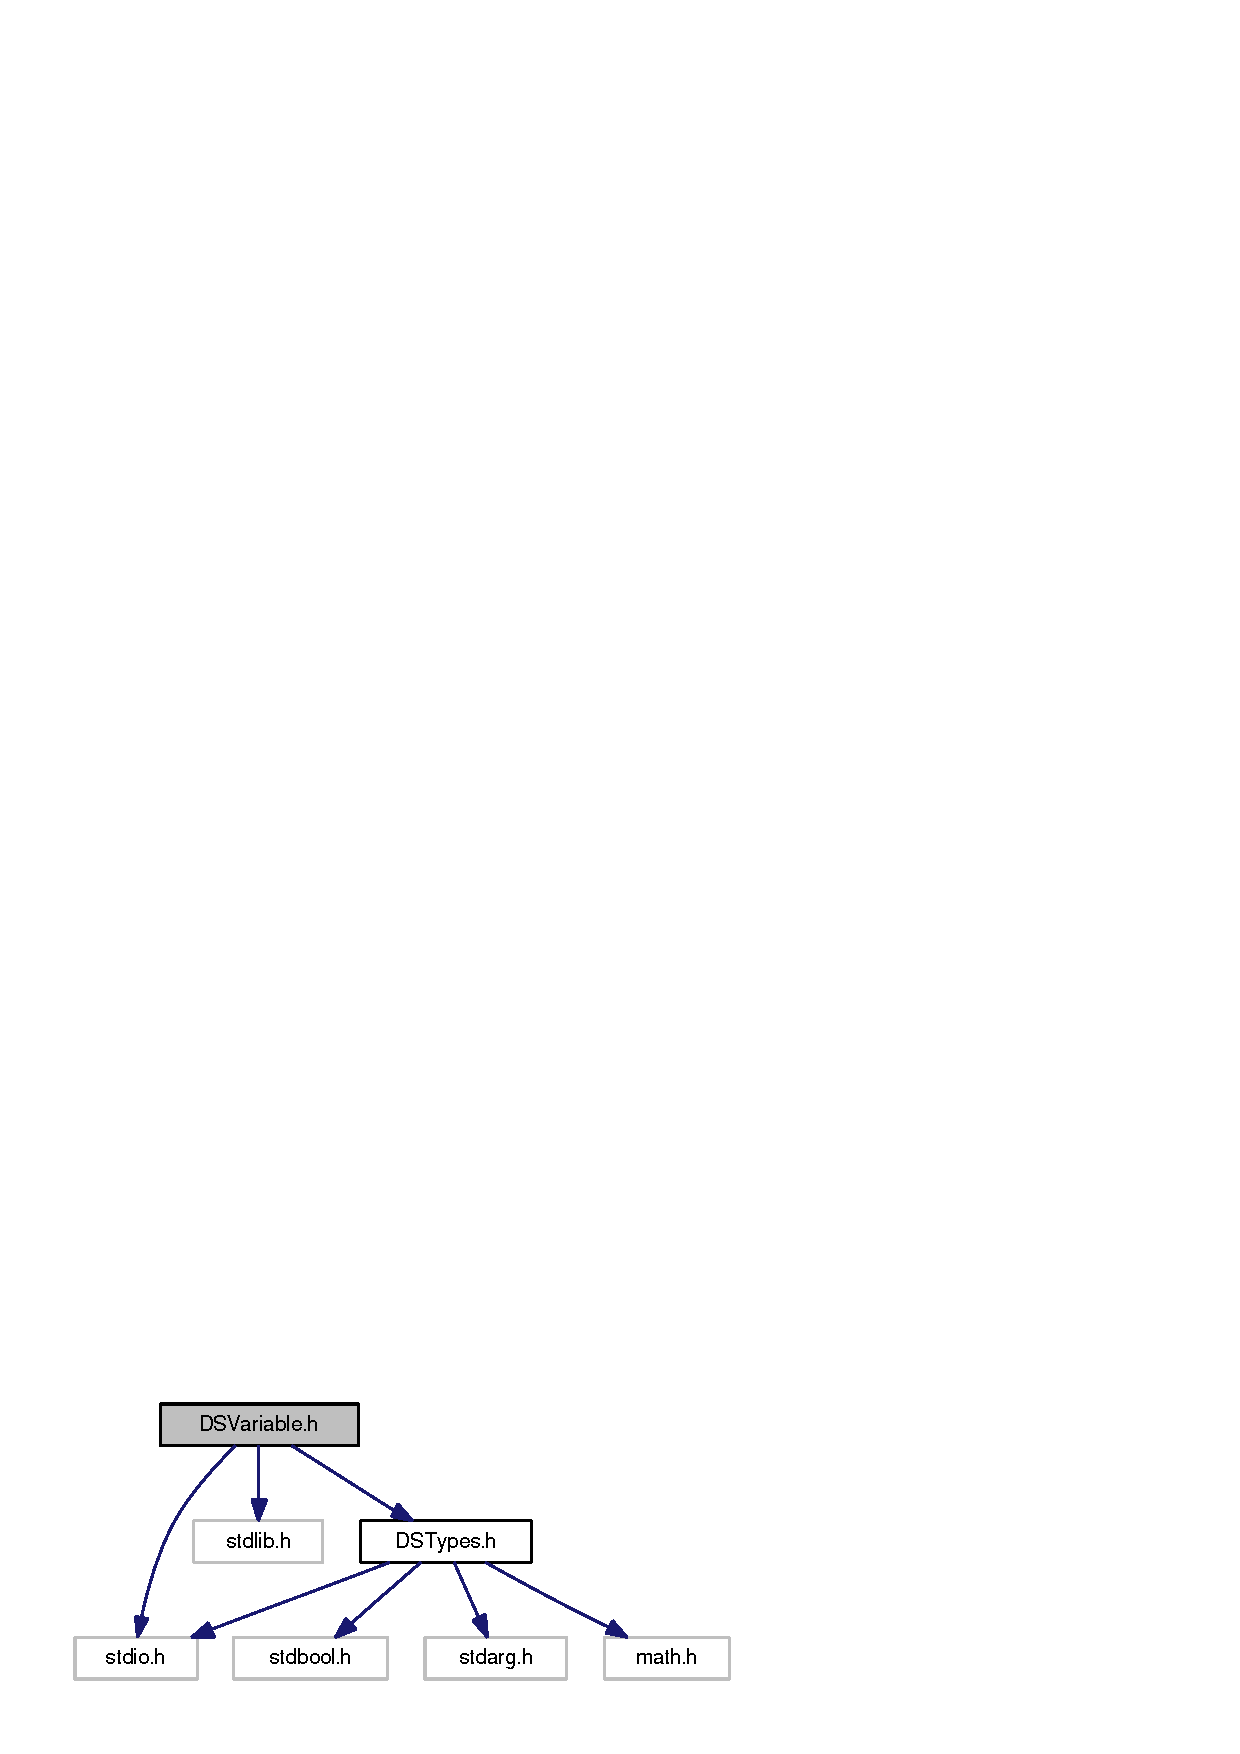
\includegraphics[width=175pt]{_d_s_variable_8h__incl}
\end{center}
\end{figure}
This graph shows which files directly or indirectly include this file:\nopagebreak
\begin{figure}[H]
\begin{center}
\leavevmode
\includegraphics[width=65pt]{_d_s_variable_8h__dep__incl}
\end{center}
\end{figure}
\subsection*{Defines}
\begin{DoxyCompactItemize}
\item 
\#define \hyperlink{group___d_s___v_a_r_i_a_b_l_e___a_c_c_e_s_s_o_r_y_ga3e1730e26b5f44a34e64d7996233d023}{DSVariableAssignValue}(x, y)~DSVariableSetValue(x, y)
\begin{DoxyCompactList}\small\item\em Macro to directly change the value of a variable. \item\end{DoxyCompactList}\item 
\#define \hyperlink{group___d_s___v_a_r_i_a_b_l_e___a_c_c_e_s_s_o_r_y_ga912df8d84202953a573824aebcf2498f}{DSVariableReturnValue}(x)~DSVariableValue(x)
\begin{DoxyCompactList}\small\item\em Macro to directly access the value of a variable. \item\end{DoxyCompactList}\item 
\hypertarget{_d_s_variable_8h_a218a0d1de0bb5ea62d7e5aa22fe50793}{
\#define {\bfseries DSVariableSetValue}(x, y)~(x)-\/$>$value = (y)}
\label{_d_s_variable_8h_a218a0d1de0bb5ea62d7e5aa22fe50793}

\item 
\hypertarget{_d_s_variable_8h_a837d0718b28591df6f518eb50d98082a}{
\#define {\bfseries DSVariableValue}(x)~(x)-\/$>$value}
\label{_d_s_variable_8h_a837d0718b28591df6f518eb50d98082a}

\item 
\hypertarget{_d_s_variable_8h_a64afbf5e8e378ef611c25084211152c4}{
\#define {\bfseries DSVariableName}(x)~(x)-\/$>$name}
\label{_d_s_variable_8h_a64afbf5e8e378ef611c25084211152c4}

\end{DoxyCompactItemize}
\subsection*{Functions}
\begin{DoxyCompactItemize}
\item 
\hyperlink{struct_d_s_variable}{DSVariable} $\ast$ \hyperlink{_d_s_variable_8h_a6f0ce189a8dc8ce46fad1d7a9b34d31f}{DSVariableAlloc} (const char $\ast$name)
\begin{DoxyCompactList}\small\item\em Creates a new \hyperlink{struct_d_s_variable}{DSVariable} with INFINITY as a default value. \item\end{DoxyCompactList}\item 
void \hyperlink{_d_s_variable_8h_aac8fadf2969493124be37a1076a2b885}{DSVariableFree} (\hyperlink{struct_d_s_variable}{DSVariable} $\ast$var)
\begin{DoxyCompactList}\small\item\em Function frees allocated memory of a \hyperlink{struct_d_s_variable}{DSVariable}. \item\end{DoxyCompactList}\item 
\hyperlink{struct_d_s_variable}{DSVariable} $\ast$ \hyperlink{_d_s_variable_8h_a1a5da69573335a86dea1e4a8a6770ea3}{DSVariableRetain} (\hyperlink{struct_d_s_variable}{DSVariable} $\ast$aVariable)
\begin{DoxyCompactList}\small\item\em Function to increase variable retain count by one. \item\end{DoxyCompactList}\item 
void \hyperlink{_d_s_variable_8h_a4d83eec85c4d9340593a359fd1d5e506}{DSVariableRelease} (\hyperlink{struct_d_s_variable}{DSVariable} $\ast$aVariable)
\begin{DoxyCompactList}\small\item\em Function to decrease variable retain count by one. \item\end{DoxyCompactList}\item 
\hypertarget{_d_s_variable_8h_af7f9c9fe77fc59c4eb4cd187d91ef171}{
\_\-\_\-deprecated \hyperlink{struct_d_s_variable}{DSVariable} $\ast$ {\bfseries DSNewVariable} (const char $\ast$name)}
\label{_d_s_variable_8h_af7f9c9fe77fc59c4eb4cd187d91ef171}

\item 
\hyperlink{struct__var_dictionary}{DSVariablePool} $\ast$ \hyperlink{_d_s_variable_8h_a4882cda43ad2d33bcafded6ed80e1fa6}{DSVariablePoolAddVariableWithName} (const char $\ast$name, \hyperlink{struct__var_dictionary}{DSVariablePool} $\ast$root)
\begin{DoxyCompactList}\small\item\em Adds a \hyperlink{struct_d_s_variable}{DSVariable} to the dictionary. \item\end{DoxyCompactList}\item 
\hyperlink{struct__var_dictionary}{DSVariablePool} $\ast$ \hyperlink{_d_s_variable_8h_aae1be18474aa9db03cb72912fd19234c}{DSVariablePoolAddVariable} (\hyperlink{struct_d_s_variable}{DSVariable} $\ast$newVar, \hyperlink{struct__var_dictionary}{DSVariablePool} $\ast$root)
\begin{DoxyCompactList}\small\item\em Adds a \hyperlink{struct_d_s_variable}{DSVariable} to the dictionary. \item\end{DoxyCompactList}\item 
\hyperlink{struct_d_s_variable}{DSVariable} $\ast$ \hyperlink{_d_s_variable_8h_ae8f75eb27aa14dda00f3251485d675ff}{DSVariablePoolVariableWithName} (const char $\ast$name, \hyperlink{struct__var_dictionary}{DSVariablePool} $\ast$root)
\begin{DoxyCompactList}\small\item\em Retrieves the variable in the dictionary with a matching name. \item\end{DoxyCompactList}\item 
void \hyperlink{_d_s_variable_8h_aaed3132c306ffc004da9f391bbd1763c}{DSVariablePoolFree} (\hyperlink{struct__var_dictionary}{DSVariablePool} $\ast$root)
\begin{DoxyCompactList}\small\item\em Function to remove all nodes in the dictionary. \item\end{DoxyCompactList}\item 
\hypertarget{_d_s_variable_8h_a0a4448f77b8bd53c9f64c48fb6be9426}{
\_\-\_\-deprecated \hyperlink{struct_d_s_variable}{DSVariable} $\ast$ {\bfseries DSVariableWithName} (const char $\ast$name, \hyperlink{struct__var_dictionary}{DSVariablePool} $\ast$root)}
\label{_d_s_variable_8h_a0a4448f77b8bd53c9f64c48fb6be9426}

\item 
void \hyperlink{_d_s_variable_8h_acbb9a673f3f91834137f2bde14911f8d}{printVarDictionary} (\hyperlink{struct__var_dictionary}{DSVariablePool} $\ast$root, DSUInteger indent)
\begin{DoxyCompactList}\small\item\em Prints the VarDictionary. \item\end{DoxyCompactList}\end{DoxyCompactItemize}


\subsection{Detailed Description}
Header file with functions for dealing with variables. Copyright (C) 2011 Jason Lomnitz.\par
\par


This file is part of the Design Space Toolbox V2 (C Library).

The Design Space Toolbox V2 is free software: you can redistribute it and/or modify it under the terms of the GNU General Public License as published by the Free Software Foundation, either version 3 of the License, or (at your option) any later version.

The Design Space Toolbox V2 is distributed in the hope that it will be useful, but WITHOUT ANY WARRANTY; without even the implied warranty of MERCHANTABILITY or FITNESS FOR A PARTICULAR PURPOSE. See the GNU General Public License for more details.

You should have received a copy of the GNU General Public License along with the Design Space Toolbox. If not, see $<$\href{http://www.gnu.org/licenses/}{\tt http://www.gnu.org/licenses/}$>$.

\begin{DoxyAuthor}{Author}
Jason Lomnitz. 
\end{DoxyAuthor}
\begin{DoxyDate}{Date}
2011 
\end{DoxyDate}


\subsection{Function Documentation}
\hypertarget{_d_s_variable_8h_a6f0ce189a8dc8ce46fad1d7a9b34d31f}{
\index{DSVariable.h@{DSVariable.h}!DSVariableAlloc@{DSVariableAlloc}}
\index{DSVariableAlloc@{DSVariableAlloc}!DSVariable.h@{DSVariable.h}}
\subsubsection[{DSVariableAlloc}]{\setlength{\rightskip}{0pt plus 5cm}{\bf DSVariable}$\ast$ DSVariableAlloc (const char $\ast$ {\em name})}}
\label{_d_s_variable_8h_a6f0ce189a8dc8ce46fad1d7a9b34d31f}


Creates a new \hyperlink{struct_d_s_variable}{DSVariable} with INFINITY as a default value. 

This function may be used throughout, in order to create new variables consistently and portably. As variables are allocated individually, it is important to not that they should be released with the accesory method. 
\begin{DoxyParams}{Parameters}
\item[{\em name}]A string with which to identify the \hyperlink{struct_d_s_variable}{DSVariable}. \end{DoxyParams}
\begin{DoxyReturn}{Returns}
The pointer to the newly allocated \hyperlink{struct_d_s_variable}{DSVariable}. 
\end{DoxyReturn}
\begin{DoxySeeAlso}{See also}
\hyperlink{struct_d_s_variable}{DSVariable} 

\hyperlink{_d_s_variable_8h_aac8fadf2969493124be37a1076a2b885}{DSVariableFree} 
\end{DoxySeeAlso}
\hypertarget{_d_s_variable_8h_aac8fadf2969493124be37a1076a2b885}{
\index{DSVariable.h@{DSVariable.h}!DSVariableFree@{DSVariableFree}}
\index{DSVariableFree@{DSVariableFree}!DSVariable.h@{DSVariable.h}}
\subsubsection[{DSVariableFree}]{\setlength{\rightskip}{0pt plus 5cm}void DSVariableFree ({\bf DSVariable} $\ast$ {\em var})}}
\label{_d_s_variable_8h_aac8fadf2969493124be37a1076a2b885}


Function frees allocated memory of a \hyperlink{struct_d_s_variable}{DSVariable}. 

This function should be used for each newDSVariable that is called. The internal structure is subject to changes in consequent versions and therefore freeing memory of DSVariables should be strictly through this function. 
\begin{DoxyParams}{Parameters}
\item[{\em var}]The pointer to the variable to free. \end{DoxyParams}
\hypertarget{_d_s_variable_8h_aae1be18474aa9db03cb72912fd19234c}{
\index{DSVariable.h@{DSVariable.h}!DSVariablePoolAddVariable@{DSVariablePoolAddVariable}}
\index{DSVariablePoolAddVariable@{DSVariablePoolAddVariable}!DSVariable.h@{DSVariable.h}}
\subsubsection[{DSVariablePoolAddVariable}]{\setlength{\rightskip}{0pt plus 5cm}{\bf DSVariablePool}$\ast$ DSVariablePoolAddVariable ({\bf DSVariable} $\ast$ {\em newVar}, \/  {\bf DSVariablePool} $\ast$ {\em root})}}
\label{_d_s_variable_8h_aae1be18474aa9db03cb72912fd19234c}


Adds a \hyperlink{struct_d_s_variable}{DSVariable} to the dictionary. 

This is the function to add DSVariables to the dictionary. Since the dictionary works alphabetically, the root of the dictionary changes and is defined by this function, and the root, be it the new one or the old one, is returned. This function is used in creating a new dictionary. 
\begin{DoxyParams}{Parameters}
\item[{\em newVar}]The pointer to the variable which is to be added to the dictionary. \item[{\em root}]The root of the dictionary. THE ROOT MAY BE REASSIGNED. If null, creates a new dictionary. \end{DoxyParams}
\begin{DoxyReturn}{Returns}
The root of the dictionary, which is likely to change. 
\end{DoxyReturn}
\begin{DoxySeeAlso}{See also}
\hyperlink{struct__var_dictionary}{\_\-varDictionary} 

DSVariableWithName 

\_\-addNewBranch 
\end{DoxySeeAlso}
\hypertarget{_d_s_variable_8h_a4882cda43ad2d33bcafded6ed80e1fa6}{
\index{DSVariable.h@{DSVariable.h}!DSVariablePoolAddVariableWithName@{DSVariablePoolAddVariableWithName}}
\index{DSVariablePoolAddVariableWithName@{DSVariablePoolAddVariableWithName}!DSVariable.h@{DSVariable.h}}
\subsubsection[{DSVariablePoolAddVariableWithName}]{\setlength{\rightskip}{0pt plus 5cm}{\bf DSVariablePool}$\ast$ DSVariablePoolAddVariableWithName (const char $\ast$ {\em name}, \/  {\bf DSVariablePool} $\ast$ {\em root})}}
\label{_d_s_variable_8h_a4882cda43ad2d33bcafded6ed80e1fa6}


Adds a \hyperlink{struct_d_s_variable}{DSVariable} to the dictionary. 

This is the function to add DSVariables to the dictionary. Since the dictionary works alphabetically, the root of the dictionary changes and is defined by this function, and the root, be it the new one or the old one, is returned. This function is used in creating a new dictionary. 
\begin{DoxyParams}{Parameters}
\item[{\em newVar}]The pointer to the variable which is to be added to the dictionary. \item[{\em root}]The root of the dictionary. THE ROOT MAY BE REASSIGNED. If null, creates a new dictionary. \end{DoxyParams}
\begin{DoxyReturn}{Returns}
The root of the dictionary, which is likely to change. 
\end{DoxyReturn}
\begin{DoxySeeAlso}{See also}
\hyperlink{struct__var_dictionary}{\_\-varDictionary} 

DSVariableWithName 

\_\-addNewBranch 
\end{DoxySeeAlso}
\hypertarget{_d_s_variable_8h_aaed3132c306ffc004da9f391bbd1763c}{
\index{DSVariable.h@{DSVariable.h}!DSVariablePoolFree@{DSVariablePoolFree}}
\index{DSVariablePoolFree@{DSVariablePoolFree}!DSVariable.h@{DSVariable.h}}
\subsubsection[{DSVariablePoolFree}]{\setlength{\rightskip}{0pt plus 5cm}void DSVariablePoolFree ({\bf DSVariablePool} $\ast$ {\em root})}}
\label{_d_s_variable_8h_aaed3132c306ffc004da9f391bbd1763c}


Function to remove all nodes in the dictionary. 

The function is RECURSIVE and frees all the nodes past the root which is passed. In theory, it could be used to clear a portion of the dictionary, yet doing so would require direct manipulation of the dictionary which is strongly discouraged. The variables themselves are NOT freed, since the dictionary does not allocate them. 
\begin{DoxyParams}{Parameters}
\item[{\em root}]The root of the dictionary which is to be cleared. \end{DoxyParams}
\begin{DoxySeeAlso}{See also}
\hyperlink{_d_s_types_8h_a67b340fa4a564cc84d27b3647ef1ad75}{DSVariablePool} 

DSVariableWithName 

\hyperlink{_d_s_variable_8h_aae1be18474aa9db03cb72912fd19234c}{DSVariablePoolAddVariable} 
\end{DoxySeeAlso}
\hypertarget{_d_s_variable_8h_ae8f75eb27aa14dda00f3251485d675ff}{
\index{DSVariable.h@{DSVariable.h}!DSVariablePoolVariableWithName@{DSVariablePoolVariableWithName}}
\index{DSVariablePoolVariableWithName@{DSVariablePoolVariableWithName}!DSVariable.h@{DSVariable.h}}
\subsubsection[{DSVariablePoolVariableWithName}]{\setlength{\rightskip}{0pt plus 5cm}{\bf DSVariable}$\ast$ DSVariablePoolVariableWithName (const char $\ast$ {\em name}, \/  {\bf DSVariablePool} $\ast$ {\em root})}}
\label{_d_s_variable_8h_ae8f75eb27aa14dda00f3251485d675ff}


Retrieves the variable in the dictionary with a matching name. 

This is the function for retriving a \hyperlink{struct_d_s_variable}{DSVariable} from a dictionary. 
\begin{DoxyParams}{Parameters}
\item[{\em name}]A string containing a NULL terminated string containing the name of the desired \hyperlink{struct_d_s_variable}{DSVariable}. \item[{\em root}]The root of the dictionary, determined during the adding of variables. \end{DoxyParams}
\begin{DoxyReturn}{Returns}
A pointer to the variable. If there is no matching variable, NULL is returned. 
\end{DoxyReturn}
\begin{DoxySeeAlso}{See also}
\_\-checkNameAtPos 

\hyperlink{_d_s_types_8h_a67b340fa4a564cc84d27b3647ef1ad75}{DSVariablePool} 

\hyperlink{_d_s_variable_8h_aae1be18474aa9db03cb72912fd19234c}{DSVariablePoolAddVariable} 
\end{DoxySeeAlso}
\hypertarget{_d_s_variable_8h_a4d83eec85c4d9340593a359fd1d5e506}{
\index{DSVariable.h@{DSVariable.h}!DSVariableRelease@{DSVariableRelease}}
\index{DSVariableRelease@{DSVariableRelease}!DSVariable.h@{DSVariable.h}}
\subsubsection[{DSVariableRelease}]{\setlength{\rightskip}{0pt plus 5cm}void DSVariableRelease ({\bf DSVariable} $\ast$ {\em aVariable})}}
\label{_d_s_variable_8h_a4d83eec85c4d9340593a359fd1d5e506}


Function to decrease variable retain count by one. 

Fast processing tree is made to decrease its retain count by one, when the retain count hits zero, the function \hyperlink{_d_s_variable_8c_aac8fadf2969493124be37a1076a2b885}{DSVariableFree()} is invoked, freeing the memory space. Fast processing tree does not have an equivalent to autorelease, forcing the developer to use greater care when directly managing memory.


\begin{DoxyParams}{Parameters}
\item[{\em aVariable}]The variable which will have its retain count reduced.\end{DoxyParams}
\begin{DoxySeeAlso}{See also}
\hyperlink{_d_s_variable_8h_a1a5da69573335a86dea1e4a8a6770ea3}{DSVariableRetain} 

\hyperlink{_d_s_variable_8h_aac8fadf2969493124be37a1076a2b885}{DSVariableFree} 
\end{DoxySeeAlso}
\hypertarget{_d_s_variable_8h_a1a5da69573335a86dea1e4a8a6770ea3}{
\index{DSVariable.h@{DSVariable.h}!DSVariableRetain@{DSVariableRetain}}
\index{DSVariableRetain@{DSVariableRetain}!DSVariable.h@{DSVariable.h}}
\subsubsection[{DSVariableRetain}]{\setlength{\rightskip}{0pt plus 5cm}{\bf DSVariable}$\ast$ DSVariableRetain ({\bf DSVariable} $\ast$ {\em aVariable})}}
\label{_d_s_variable_8h_a1a5da69573335a86dea1e4a8a6770ea3}


Function to increase variable retain count by one. 

Variables utilize a similar memory management system used in Objective-\/C NSObject subclasses, where objects a retained/released.


\begin{DoxyParams}{Parameters}
\item[{\em aVariable}]The variable which will have its retain count increased.\end{DoxyParams}
\begin{DoxyReturn}{Returns}
The same variable which received the retain count increase is returned, for convinience.
\end{DoxyReturn}
\begin{DoxySeeAlso}{See also}
\hyperlink{_d_s_variable_8h_a4d83eec85c4d9340593a359fd1d5e506}{DSVariableRelease} 
\end{DoxySeeAlso}
\hypertarget{_d_s_variable_8h_acbb9a673f3f91834137f2bde14911f8d}{
\index{DSVariable.h@{DSVariable.h}!printVarDictionary@{printVarDictionary}}
\index{printVarDictionary@{printVarDictionary}!DSVariable.h@{DSVariable.h}}
\subsubsection[{printVarDictionary}]{\setlength{\rightskip}{0pt plus 5cm}void printVarDictionary ({\bf DSVariablePool} $\ast$ {\em root}, \/  DSUInteger {\em indent})}}
\label{_d_s_variable_8h_acbb9a673f3f91834137f2bde14911f8d}


Prints the VarDictionary. 

A debugging function which prints the dictionary structure to the stderr file 
\printindex
\end{document}
